\documentclass[openany,preprint,11pt]{book}

\usepackage{amsthm,amsmath,amssymb,amsfonts,amscd,amsbsy}
\usepackage[ruled,noline,linesnumbered]{algorithm2e}
\usepackage{cancel}
\usepackage{color}
\usepackage{fullpage}
\usepackage{graphicx}
\usepackage{hyperref}
\usepackage[tight]{subfigure}
\usepackage{titlesec}

\DeclareGraphicsExtensions{.jpg,.png,.pdf}
\DeclareGraphicsRule{*}{mps}{*}{}
\graphicspath{{./fig/}}



% bold letters
\newcommand{\bola}{\mathbf{a}}
\newcommand{\bolc}{\mathbf{c}}
\newcommand{\bolf}{\mathbf{f}}
\newcommand{\bolg}{\mathbf{g}}
\newcommand{\boll}{\mathbf{l}}
\newcommand{\bolq}{\mathbf{q}}
\newcommand{\bolp}{\mathbf{p}}
\newcommand{\bolu}{\mathbf{u}}
\newcommand{\bolv}{\mathbf{v}}
\newcommand{\bolw}{\mathbf{w}}
\newcommand{\bolz}{\mathbf{z}}

\newcommand{\bolA}{\mathbf{A}}
\newcommand{\bolB}{\mathbf{B}}
\newcommand{\bolC}{\mathbf{C}}
\newcommand{\bolD}{\mathbf{D}}
\newcommand{\bolE}{\mathbf{E}}
\newcommand{\bolF}{\mathbf{F}}
\newcommand{\bolG}{\mathbf{G}}
\newcommand{\bolH}{\mathbf{H}}
\newcommand{\bolI}{\mathbf{I}}
\newcommand{\bolJ}{\mathbf{J}}
\newcommand{\bolK}{\mathbf{K}}
\newcommand{\bolL}{\mathbf{L}}
\newcommand{\bolM}{\mathbf{M}}
\newcommand{\bolN}{\mathbf{N}}
\newcommand{\bolO}{\mathbf{O}}
\newcommand{\bolP}{\mathbf{P}}
\newcommand{\bolQ}{\mathbf{Q}}
\newcommand{\bolR}{\mathbf{R}}
\newcommand{\bolS}{\mathbf{S}}
\newcommand{\bolT}{\mathbf{T}}
\newcommand{\bolU}{\mathbf{U}}
\newcommand{\bolV}{\mathbf{V}}
\newcommand{\bolW}{\mathbf{W}}
\newcommand{\bolX}{\mathbf{X}}
\newcommand{\bolY}{\mathbf{Y}}
\newcommand{\bolZ}{\mathbf{Z}}

% bold symbols
\newcommand{\bolalpha}{\boldsymbol{\alpha}}
\newcommand{\bolbeta}{\boldsymbol{\beta}}
\newcommand{\boleta}{\boldsymbol{\eta}}
\newcommand{\bolpsi}{\boldsymbol{\psi}}

% shadowed letters
\newcommand{\PP}{\mathbb{P}}
\newcommand{\RR}{\mathbb{R}}
\newcommand{\CC}{\mathbb{C}}
\newcommand{\ZZ}{\mathbb{Z}}

% mathcal letters
\newcommand{\calA}{\mathcal{A}}
\newcommand{\calB}{\mathcal{B}}
\newcommand{\calC}{\mathcal{C}}
\newcommand{\calD}{\mathcal{D}}
\newcommand{\calE}{\mathcal{E}}
\newcommand{\calF}{\mathcal{F}}
\newcommand{\calG}{\mathcal{G}}
\newcommand{\calH}{\mathcal{H}}
\newcommand{\calI}{\mathcal{I}}
\newcommand{\calJ}{\mathcal{J}}
\newcommand{\calK}{\mathcal{K}}
\newcommand{\calL}{\mathcal{L}}
\newcommand{\calM}{\mathcal{M}}
\newcommand{\calN}{\mathcal{N}}
\newcommand{\calO}{\mathcal{O}}
\newcommand{\calP}{\mathcal{P}}
\newcommand{\calQ}{\mathcal{Q}}
\newcommand{\calR}{\mathcal{R}}
\newcommand{\calS}{\mathcal{S}}
\newcommand{\calT}{\mathcal{T}}
\newcommand{\calU}{\mathcal{U}}
\newcommand{\calV}{\mathcal{V}}
\newcommand{\calW}{\mathcal{W}}
\newcommand{\calX}{\mathcal{X}}
\newcommand{\calY}{\mathcal{Y}}
\newcommand{\calZ}{\mathcal{Z}}


% derivatives
\newcommand{\pp}[2]{\frac{\partial #1}{\partial #2}}
\newcommand{\dd}[2]{\frac{d #1}{d #2}}


% fraction shortcut
\newcommand{\f}[2]{\frac{#1}{#2}}
\newcommand{\slfrac}[2]{\left.#1\middle/#2\right.}

% common operators
\newcommand{\vvvert}{|\kern-1pt|\kern-1pt|}
\newcommand{\enorm}[1]{\vvvert #1 \vvvert}


% matrices
\newcommand{\bmat}[1]{\left(\begin{array}{#1}}
\newcommand{\emat}{\end{array}\right)} 



\newcommand{\blist}{\begin{list}{\ballrefb}{\leftmargin=2.0em}
  \setlength{\itemsep}{2pt}
  \setlength{\parskip}{0pt}}
\newcommand{\elist}{\end{list}}



% common format strings
\def\etal{{\it et al.}}
\def\ie{{\it i.e.}}
\def\eg{{\it e.g.}}


\DeclareMathOperator*{\arginf}{arg\,inf}
\DeclareMathOperator*{\argsup}{arg\,sup}
\DeclareMathOperator*{\argmax}{arg\,max}
\DeclareMathOperator*{\argmin}{arg\,min}


\renewcommand{\chaptername}{Lecture}
\newcommand{\disclaimer}{\copyright2018 Masayuki Yano.  Prepared for AER1418 Variational Methods for PDEs taught at the University of Toronto.}

%\titleformat{\chapter}[display]
%            {\huge\bfseries}{Lecture \thechapter}{0.5ex}
%            {} % before code
%            {\disclaimer} % after code
  
\theoremstyle{definition}
\newtheorem{theorem}{Theorem}[chapter]
\newtheorem{lemma}[theorem]{Lemma}
\newtheorem{proposition}[theorem]{Proposition}
\newtheorem{remark}[theorem]{Remark}
\newtheorem{definition}[theorem]{Definition}
\newtheorem{corollary}[theorem]{Corollary}
\newtheorem{assumption}[theorem]{Assumption}
\newtheorem{example}[theorem]{Example}

\begin{document}
\begin{center}
  \phantom{.}

  \vspace{20ex}
  \begin{huge}
    AER1418: Variational Methods for PDEs \\[2ex]
    Lecture Notes \\[2ex]
  \end{huge}

  \begin{large}
    Version 0.0 (Winter 2018) \\[5ex]
    Masayuki Yano \\[2ex]
    University of Toronto \\
    Institute for Aerospace Studies \\[2ex]
    \copyright2018 Masayuki Yano, University of Toronto.
  \end{large}
  

\end{center}



\clearpage
%\include{acknowledgment}
\tableofcontents

\chapter{Introduction: Poisson equation in one dimension}

\disclaimer

\section{Motivation}
In this lecture, we provide a brief overview of a variational formulation and the associated finite element approximation using a concrete example: one-dimensional Poisson equation. The goal is to illustrate the main ideas without complexities associated with higher dimensions and more general equations; we also defer some of the technical discussions to later lectures.

\section{Model problem: strong form}
\label{sec:intro_strong}
We consider a taut string with fixed ends subjected to a distributed transverse load as shown in Figure~\ref{fig:intro_string}.  Given an appropriate normalization, the shape of the string can be modeled as a one-dimensional Poisson equation on $\Omega \equiv (0,1)$: find $u$ such that
\begin{align}
  - \dd{^2u}{x^2} &= f \quad \text{in } \Omega  \label{eq:intro_strong} \\
  u(x=0) &= 0 \notag , \\
  u(x=1) &= 0 \notag ,
\end{align}
where $f$ is associated with the transverse load.  We may integrate the ODE twice to confirm the existence and uniqueness of the solution.  We will refer to this particular form of the problem as the \emph{strong form}.

\begin{figure}
  \centering
  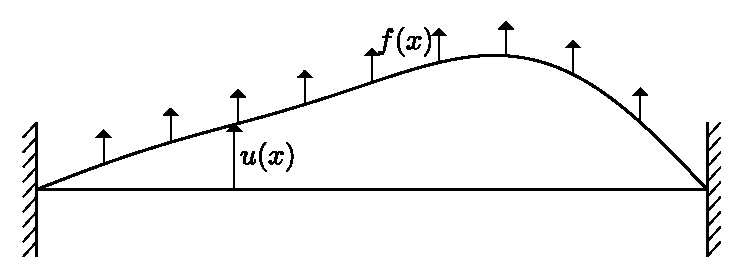
\includegraphics[width=0.6\textwidth]{poisson_string}
  \caption{Taut-string problem modeled by the Poisson equation. \label{fig:intro_string}}
\end{figure}

%% One concrete application of the model equation is an elastic bar with fixed ends subjected to distributed force.  The bar is then modeled as
%% \begin{align*}
%%   \sigma &= EA \dd{u}{x} \quad &\text{(Hooke's law)} \\
%%   \dd{\sigma}{x} &= f \quad &\text{(force equilibrium)} \\
%%   u(x=0) = u(x=1) &=0 \quad &\text{(fixed ends)};
%% \end{align*}
%% here $u$ is the displacement, $\sigma$ is the internal force (i.e. area weighted stress), $E$ is the Young's modulus, $A$ is the cross sectional area, and $f$ is the distributed external force. We recognize that the problem fits in the model equation~\eqref{eq:intro_strong}.

\section{Minimization form}
We now consider a \emph{minimization form} of the model problem~\eqref{eq:intro_strong}.  To this end, we first introduce a linear space
\begin{equation}
  \calV \equiv \{ v \ | \
   v \text{ is continuous, } 
   \int_\Omega \left(\dd{v}{x}\right)^2 dx \text{ is bounded, and } % \text{ is piecewise continuous and bounded on $\Omega$, and } \\
   v(x=0) = v(x=1) = 0 \}.
  \label{eq:intro_V}
\end{equation}
The first two conditions are related to the smoothness of the solution sought, and the last condition imposes the boundary condition.
We then define a functional $J: \calV \to \RR$ given by
\begin{equation}
  J(w) \equiv \frac{1}{2} \int_\Omega \left( \dd{w}{x} \right)^2 dx - \int_\Omega f w dx \quad \forall w \in \calV.
  \label{eq:intro_J}
\end{equation}
Our \emph{minimization problem} is as follows: find $u \in \calV$ such that
\begin{equation}
  u = \argmin_{w \in \calV} J(w).
  \label{eq:intro_min}
\end{equation}
For a physical system with intrinsic energy, such as the taut-string problem in Section~\ref{eq:intro_strong}, the functional $J$ represents the total energy in the system; $\int_\Omega (\pp{w}{x})^2 dx$ is the internal energy and $\int_\Omega f w dx$ is the external work.  Our minimization statement is hence a statement of energy minimization at the equilibrium. 

We can readily show that the solution to the strong form~\eqref{eq:intro_strong} solves the minimization problem~\eqref{eq:intro_min}.  To see this, let $w = u + v$, where $u \in \calV$ is the solution to~\eqref{eq:intro_strong} and $v$ is an arbitrary function in $\calV$.  We then note that $J(w) = J(u+v)$ can be decomposed into three terms:
\begin{align*}
  J(u+v) &= \frac{1}{2} \int_{\Omega} \left( \dd{(u+v)}{x} \right)^2 dx - \int_\Omega f(u+v) dx \\
  &= \underbrace{ \frac{1}{2} \int_{\Omega} \left( \dd{u}{x} \right)^2 dx - \int_\Omega f u dx }_{J(u)}
  + \underbrace{ \int_{\Omega} \dd{v}{x} \dd{u}{x} dx - \int_\Omega f v dx }_{J'(u;v) \text{ --- first variation}}
  + \underbrace{ \frac{1}{2} \int_{\Omega} \left( \dd{v}{x} \right)^2 dx }_{> 0 \text{ for } v \neq 0}.
\end{align*}
Here, $J'(u;v)$ denotes the first variation of $J$ at $u$ in the direction $v$.  We integrate by parts $J'(u;v)$ to obtain
\begin{align*}
  J'(u;v) &= \int_{\Omega} \dd{v}{x} \dd{u}{x} dx - \int_\Omega f v dx
  =
  - \int_{\Omega} v ( \underbrace{ \dd{^2u}{x^2} + f}_{= 0 \text{ as $u$ solves \eqref{eq:intro_strong}}} ) dx + \underbrace{ \left[ v \dd{u}{x} \right]_{x=0}^1 }_{= 0 \text{ as $v$ is in $\calV$}}
  = 0;
\end{align*}
in other words, if $u$ is the solution to the strong form~\eqref{eq:intro_strong}, then $J'(u;v) = 0$ for all $v \in \calV$. It thus follows
\begin{align*}
  J(u + v) = J(u) + \frac{1}{2} \int_\Omega \left( \dd{v}{x} \right)^2 dx
  > J(u)  \quad \forall v \neq 0.
\end{align*}
The solution $u$ to the strong form~\eqref{eq:intro_strong} is the minimizer of the functional~\eqref{eq:intro_J} and hence the solution to the minimization form~\eqref{eq:intro_min}.

While the solution to the strong form~\eqref{eq:intro_strong} is also the solution to the minimization form~\eqref{eq:intro_min}, the converse is not true in general.  In fact, the minimization form admits more general loads $f$ and associated solutions than the strong form.

\section{Variational form}
We now consider a \emph{variational form} of the model problem~\eqref{eq:intro_strong}. As in the minimization form, we work with the function space~$\calV$ defined in~\eqref{eq:intro_V}. We then introduce a \emph{bilinear form} $a: \calV \times \calV \to \RR$,
\begin{equation}
  a(w,v) \equiv \int_{\Omega} \dd{v}{x} \dd{w}{x} dx \quad \forall w, v \in \calV,
  \label{eq:intro_a}
\end{equation}
and a \emph{linear form} $\ell: \calV \to \RR$,
\begin{equation}
  \ell(v) \equiv \int_{\Omega} v f dx \quad \forall v \in \calV.
  \label{eq:intro_ell}
\end{equation}
The form $\ell: \calV \to \RR$ is called a \emph{linear form} because it is linear in the argument in the sense that
\begin{equation*}
  \ell(\alpha w + \beta v) = \alpha \ell(w) + \beta \ell(v) \quad \forall w,v \in \calV, \ \forall \alpha, \beta \in \RR.
\end{equation*}
The form $a: \calV \times \calV \to \RR$ is called a \emph{bilinear form} because 
\begin{align*}
  a(w, \tilde v) & \text{ is a linear form in $w$ for a fixed $\tilde v$, and} \\
  a(\tilde w, v) & \text{ is a linear form in $v$ for a fixed $\tilde w$}.
\end{align*}
Our \emph{variational problem} is as follows: find $u \in \calV$ such that
\begin{equation}
  a(u,v) = \ell(v) \quad \forall v \in \calV.
  \label{eq:intro_var}
\end{equation}
This variational form of the problem is also called the \emph{weak form}. The variational problem has a unique solution; we will study the well-posedness of the problem in subsequent lectures.

We can readily show that $u \in \calV$ is the solution to the variational problem~\eqref{eq:intro_var} if and only if it is the solution to the minimization problem~\eqref{eq:intro_min}.  Suppose that $u \in \calV$ is the solution to the variational problem~\eqref{eq:intro_var}.  Then, for $w = u + v$ for any $v \in \calV$, we obtain
\begin{align*}
  J(w) = J(u + v) = J(u) + \underbrace{ \int_{\Omega} \dd{v}{x} \dd{u}{x} dx - \int_\Omega f v dx}_{= a(u,v) - \ell(v) = 0 \ \forall v \in \calV \text{ by \eqref{eq:intro_var}}}
  + \underbrace{ \frac{1}{2} \int_{\Omega} \left( \dd{v}{x} \right)^2 dx }_{> 0 \text{ for } v \neq 0} > J(u) \quad \forall v \neq 0;
\end{align*}
hence the solution $u \in \calV$ of the variational problem~\eqref{eq:intro_var} solves the minimization problem~\eqref{eq:intro_min}. 
Conversely, suppose $u \in \calV$ is the solution to the minimization problem~\eqref{eq:intro_min}.  Then, we know that $u$ must be a stationary point of $J$: i.e., $J'(u;v) = 0$, $\forall v \in \calV$; we hence require
\begin{equation*}
  J'(u;v) \equiv
  \int_{\Omega} \dd{v}{x} \dd{u}{x} dx
  - \int_{\Omega} f v dx
  = a(u,v) - \ell(v) = 0 \quad \forall v \in \calV,
\end{equation*}
which the exact condition of our variational problem~\eqref{eq:intro_var}. Hence we conclude that $u \in \calV$ is the solution to~\eqref{eq:intro_var} if and only if it is the solution to~\eqref{eq:intro_min}.  We will soon see that we can derive a finite element approximation from either~\eqref{eq:intro_var} or \eqref{eq:intro_min}.

\section{Finite element (FE) approximation}
In order to construct a finite element (FE) approximation, we must choose a suitable subspace of $\calV$ that well approximates $\calV$ and is amenable to computer implementation. To this end, we first \emph{tessellate} (or \emph{triangulate}) the domain $\Omega \equiv (0,1)$ into $N+1$ non-overlapping segments; we introduce points
\begin{equation*}
  0 \equiv x_0 < x_1 < \cdots < x_N < x_{N+1} \equiv 1
\end{equation*}
and segments
\begin{equation*}
  K_i \equiv (x_{i-1}, x_i) \quad i = 1,\dots,N+1.
\end{equation*}
We denote the \emph{tessellation} of the domain $\Omega$, which comprises collection of segments, by
\begin{equation}
  \calT_h \equiv \{ K_i \}_{i=1}^{N+1}.
  \label{eq:intro_Th}
\end{equation}
We denote the length of each segment by $h_i \equiv x_i - x_{i-1}$, $i = 1,\dots,N+1$; a tessellation $\calT_h$ is characterized by the maximum segment length $h \equiv \max_{i=\{ 1,\dots,N+1\}} h_i$.

We now introduce a space of piecewise linear functions associated with our tessellation $\calT_h$ and that belong to $\calV$:
\begin{equation}
  \calV_h \equiv \{ v \in \calV \ | \ v|_{K_i} \in \PP^1(K_i), \ i = 1,\dots,N+1\}.
  \label{eq:intro_Vh}
\end{equation}
We make a few observations.  First, we require $v$ is in $\calV$ defined in \eqref{eq:intro_V}: (i) $v$ must be continuous, (ii) $\dd{v}{x}$ must be piecewise continuous and bounded, and (iii) $v$ must vanish at the boundaries.  Second, we require $v$ restricted to segment $K_i$ to be in $\PP^1(K_i)$; here, $\PP^1(K_i)$ denotes the space of linear polynomials over $K_i$.  Hence, any function in $\calV_h \subset \calV$ is continuous, piecewise linear, and vanishes at the boundaries. An example of a function in $\calV_h$ is shown in Figure~\ref{fig:poisson_fe_space}.

\begin{figure}
  \centering
  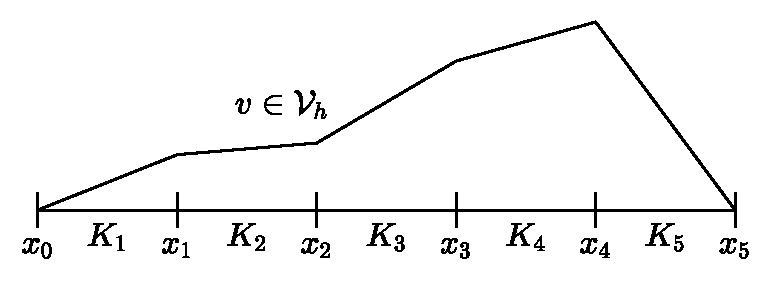
\includegraphics[width=0.6\textwidth]{poisson_fe_space}
  \caption{Linear finite element space for $N = 4$.}
  \label{fig:poisson_fe_space}
\end{figure}

We can now state our FE approximation problem in either the minimization form or the variational form.  The FE minimization form is as follows: find $u_h \in \calV_h$ such that
\begin{equation}
  u_h = \argmin_{v \in \calV_h} J(v),
  \label{eq:intro_min_fe}
\end{equation}
where $J: \calV \to \RR$ is the energy functional~\eqref{eq:intro_J}. In words, we seek the minimizer in the subspace $\calV_h$ of $\calV$.  Note that $v \in \calV_h$ is an admissible argument of $J$ since $\calV_h \subset \calV$. Similarly, the FE variational form is as follows: find $u_h \in \calV_h$ such that
\begin{equation}
  a(u_h,v) = \ell(v) \quad \forall v \in \calV_h,
  \label{eq:intro_var_fe}
\end{equation}
where $a: \calV \times \calV \to \RR$ and $\ell: \calV \to \RR$ are biilnear form~\eqref{eq:intro_a} and linear form~\eqref{eq:intro_ell}, respectively.  As before, $u_h \in \calV_h$ is the solution to the FE minimization problem~\eqref{eq:intro_min_fe} if and only if it is the solution to the FE variational problem~\eqref{eq:intro_var_fe}. We will henceforth refer to $u_h$ as the \emph{finite element solution}.


\section{Finite element approximation: implementation}
We now wish to implement~\eqref{eq:intro_var_fe} (or equivalently~\eqref{eq:intro_min_fe}).  To this end, we introduce a \emph{basis} for $\calV_h$ defined in~\eqref{eq:intro_Vh}.  A convenient basis for $\calV_h$ is a \emph{Lagrange basis} $\{\phi_i\}_{i=1}^N$ such that 
\begin{equation*}
  \phi_i(x_j) = \delta_{ij} \equiv  \begin{cases}
    1 \quad j = i \\
    0 \quad j\neq i
  \end{cases},
  \quad j = 0,\dots,N+1;
\end{equation*}
in words, $\phi_i$ is a continuous piecewise linear function that is takes the value of 1 at the interpolation point $x_i$ and the value of 0 at all other interpolation points.  The basis functions are shown in Figure~\ref{fig:poisson_1d_basis}.

\begin{figure}
  \centering
  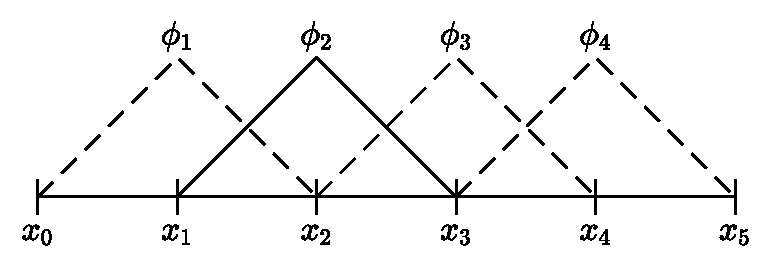
\includegraphics[width=0.6\textwidth]{poisson_1d_basis}
  \caption{Basis functions for a linear finite element space for $N = 4$.}
  \label{fig:poisson_1d_basis}
\end{figure}

We can show that $\{ \phi_i \}_{i=1}^N$ is indeed a basis for $\calV_h$: the set (i) is linearly independent and (ii) spans $\calV_h$. To show the set is linearly independent, we must show that $\sum_{i=1}^n c_i \phi_i(x) = 0$ implies $c_i = 0$, $i = 1,\dots,N$; the statement holds because, for $\sum_{i=1}^n c_i \phi_i(x) = 0$, we must have $\sum_{i=1}^n c_i \phi_i(x_j) = \sum_{i=1}^n c_i \delta_{ij} = c_j = 0$, $j = 1,\dots,N$. To show the set spans $\calV_h$, we observe that any $v \in \calV_h$ can be expressed as
\begin{equation*}
  v = \sum_{i=1}^N \hat v_i \phi_i
\end{equation*}
for $\hat v_i \equiv v(x_i)$. (The coefficients are also unique because the set is linearly independent.)  We hence conclude that $\{\phi_i\}_{i=1}^N$ is a basis for $\calV_h$. 

%% We can readily show that $\{ \phi_i \}_{i=1}^N$ is indeed a basis for $\calV_h$: i.e., $\calV_h = \text{span}\{ \phi_i \}_{i=1}^N$ and $\{\phi_i\}_{i=1}^N$ is linearly independent. We note that for \emph{any} function $v \in \calV_h$, there exists a \emph{unique} coefficients $\hat v \in \RR^N$ such that 
%% \begin{equation*}
%%   v(x) = \sum_{i=1}^N \hat v_i \phi_i(x), \quad x \in \Omega.
%% \end{equation*}
%% In particular, the choice $\hat v_i = v(x_i)$ yields the desired equality.

We now restate the FE variational problem~\eqref{eq:intro_var_fe} using the basis and associated coefficients.  Specifically, we represent $u_h \in \calV_h$ and $v \in \calV_h$ as 
\begin{align}
  u_h &\equiv \sum_{j=1}^N \hat u_{h,j} \phi_j \label{eq:intro_uh_rep} \\
   v &\equiv \sum_{i=1}^N \hat v_i \phi_i \notag
\end{align}
for some $\hat u_h \in \RR^N$ and $\hat v \in \RR^N$, and consider the following equivalent problem: find $\hat u_h \in \RR^N$ such that
\begin{equation}
  a(\sum_{j=1}^N \hat u_{h,j} \phi_j, \sum_{i=1}^N \hat v_i \phi_i) - \ell(\sum_{i=1}^N \hat v_i \phi_i)
  =
  \sum_{i=1}^N \sum_{j=1}^N \hat v_i a(\phi_j, \phi_i) \hat u_{h,j} -
  \sum_{i=1}^N \hat v_i \ell(\phi_i) = 0 \quad \forall \hat v \in \RR^N.
  \label{eq:intro_fe_disc_step_1}
\end{equation}
Here, we have appealed to the bilinearity and linearity of $a(\cdot,\cdot)$ and $\ell(\cdot)$, respectively. We then note that in~\eqref{eq:intro_fe_disc_step_1} we can replace the condition $\forall \hat v \in \RR^N$ with an equivalent condition that the statement hold for $\hat v \in \{e_i \}_{i=1}^N$ for $\{e_i\}_{i=1}^N$ the canonical basis of $\RR^N$ (i.e.~$e_i \in \RR^N$ has $1$ in the $i$-th entry and $0$ elesewhere). Then, we can restate~\eqref{eq:intro_fe_disc_step_1} as follows: find $\hat u_h \in \RR^N$ such that
\begin{equation}
  \sum_{j=1}^N a(\phi_j,\phi_i) \hat u_{h,j} = \ell(\phi_i) \quad  \forall i = 1,\dots,N.
  \label{eq:intro_sys}
\end{equation}
We can also rewrite the linear system in the matrix form:
\begin{equation*}
  \underbrace{ \bmat{ccc}
  a(\phi_1,\phi_1) & \cdots & a(\phi_N,\phi_1) \\
  \vdots & \ddots & \vdots \\
  a(\phi_1,\phi_N) & \cdots & a(\phi_N,\phi_N) \\
  \emat
  }_{A_h \in \RR^{N \times N}}
  \underbrace{ \bmat{c} \hat u_{h,1}  \\ \vdots \\ \hat u_{h,N} \emat }_{\hat u_h \in \RR^N}
  =
  \underbrace{ \bmat{c} \ell(\phi_1) \\ \vdots \\ \ell(\phi_N) \emat }_{\hat f_h \in \RR^N},
\end{equation*}
or, more concisely,
\begin{equation*}
  A_h \hat u_h = f_h.
\end{equation*}
The matrix $A_h$ is called the \emph{stiffness matrix} and the vector $f_h$ is called the \emph{load vector}.% The linear system is in fact \emph{symmetric positive definite} (SPD) and hence has a unique solution.

%\section{Solution of $A_h \hat u_h = f_h$}

We now take a closer look at the matrix $A_h \in \RR^{N \times N}$ associated with our particular choice of the basis $\{\phi_i\}_{i=1}^N$.  We decompose the matrix into four parts: main diagonal, superdiagonal, subdiagonal, and all other entries.  The diagonal entries are given by 
\begin{equation*}
  a(\phi_i,\phi_i) = \int_{x_{i-1}}^{x_{i+1}} \dd{\phi_i}{x} \dd{\phi_i}{x} dx
  = \int_{x_{i-1}}^{x_{i}} \left( \frac{1}{h_i} \right)^2 dx +
  \int_{x_{i}}^{x_{i+1}} \left( - \frac{1}{h_{i+1}} \right)^2 dx
  = \frac{1}{h_i} + \frac{1}{h_{i+1}}, \quad i = 1,\dots,N.
\end{equation*}
The superdiagonal entries are given by
\begin{equation*}
  a(\phi_i,\phi_{i+1}) =
  \int_{x_i}^{x_{i+1}} \dd{\phi_i}{x} \dd{\phi_{i+1}}{x} dx
  = \int_{x_i}^{x_{i+1}} \left( - \frac{1}{h_i} \right) \left( \frac{1}{h_i} \right) dx
  = - \frac{1}{h_i}, \quad i = 1,\dots,N-1.
\end{equation*}
The subdiagonal entries are given by
\begin{equation*}
  a(\phi_{i+1},\phi_i) =
  \int_{x_i}^{x_{i+1}} \dd{\phi_{i+1}}{x} \dd{\phi_i}{x} dx
  = \int_{x_i}^{x_{i+1}}  \left( \frac{1}{h_i} \right) \left( - \frac{1}{h_i} \right) dx
  = - \frac{1}{h_i}, \quad i = 1,\dots,N-1.
\end{equation*}
All other entries are zero because $\phi_i$ and $\phi_j$ do not overlap for $|i -j| > 1$.

We now consider the simple case of equispaced nodes so that $h_i = h$, $\forall i = 1,\dots,N$.  The associated stiffness matrix is
\begin{equation*}
  A_h = \frac{1}{h} \bmat{ccccc} 2 & -1 \\ -1 & 2 & -1 \\ & \ddots & \ddots & \ddots \\ & &-1 & 2 & -1 \\ &&& -1 & 2 \emat.
\end{equation*}
We observe that the matrix is \emph{sparse} and in particular \emph{tridiagonal}.  Moreover, this matrix is symmetric positive definite.  The symmetry is obvious from inspection; the positive definiteness follows from 
\begin{align*}
  \hat v^T A_h \hat v
  &=
  \frac{1}{h} \left(
  2\sum_{i=1}^N \hat v_i^2 - 2\sum_{i=1}^{N-1} \hat v_i\hat v_{i+1} 
  \right)
  =
  \frac{1}{h} \left(
  \hat v_1^2 + \hat v_{N}^2 + \sum_{i=1}^{N-1} (\hat v_i - \hat v_{i+1})^2 
  \right)
  > 0 \quad \forall \hat v \neq 0.
\end{align*}
Hence the solution exists and is unique.  The storage requirement for the tridiagonal system is $\calO(N)$, and the solution to $A_h \hat u_h = f_h$ can be obtained using the Thomas algorithm in $\calO(N)$ floating point operations.  Given the solution  $\hat u_h \in \RR^N$ to the linear system, our finite element solution $u_h \in \calV_h$ to~\eqref{eq:intro_var_fe} (or equivalently~\eqref{eq:intro_min_fe}) is given by the representation~\eqref{eq:intro_uh_rep}.

\section{An error estimate: optimality and polynomial approximation}
We now assess how accurately our finite element solution $u_h \in \calV_h$ to~\eqref{eq:intro_var_fe} (or equivalently~\eqref{eq:intro_min_fe}) approximates the solution $u \in \calV$ to~\eqref{eq:intro_var} (or equivalently~\eqref{eq:intro_min}).  To this end, we need to first define a norm with which we measure the ``closeness'' of the approximation. We in particular introduce the \emph{energy norm} associated with the model problem,
\begin{equation*}
  \enorm{v} \equiv \sqrt{a(v,v)}  = \left( \int_{\Omega} \left( \dd{v}{x} \right)^2 dx \right)^{1/2} \quad \forall v \in \calV.
\end{equation*}
Because $\enorm{ \cdot }$ is the induced norm associated with an inner product $a(\cdot,\cdot)$ over $\calV$, it is indeed a proper norm that satisfies i) scalability, ii) triangle inequality, and iii) positivity.  

We next state a key ingredient of the FE error estimate: \emph{Galerkin orthogonality}: since $\ell(v) = a(u,v)$, $\forall v \in \calV$, the FE variational statement~\eqref{eq:intro_var_fe} implies
\begin{equation*}
  \ell(v) - a(u_h,v) = a(u,v) - a(u_h,v) = a(u-u_h,v) \quad \forall v \in V_h;
\end{equation*}
the relationship is called Galerkin orthogonality because it states that the error $u - u_h$ is orthogonal to the space $\calV_h$ in the inner product $a(\cdot,\cdot)$. We now observe that, for any $w_h \in \calV_h$,
\begin{align*}
  \enorm{u-u_h}^2
  &=
  a(u-u_h, u-w_h) + a(u-u_h,w_h - u_h)
  \\
  &=
  a(u-u_h, u - w_h) & \text{(Galerkin orthogonality)}
  \\
  &\leq  \enorm{u - u_h} \enorm{u - w_h}. & \text{(Cauchy-Schwarz inequality)}.
\end{align*}
It follows that
\begin{equation}
  \enorm{u - u_h} \leq \enorm{u - w_h} \quad \forall w_h \in \calV_h,
  \label{eq:intro_fe_opt}
\end{equation}
or, equivalently,
\begin{equation*}
  \enorm{u-u_h} = \inf_{w_h \in \calV_h} \enorm{u - w_h}.
\end{equation*}
We observe that the FE approximation $u_h \in \calV_h$ is \emph{optimal} in the energy norm in the sense that it is the closest approximation to the solution $u \in \calV$ out of all elements in $\calV_h$.  In other words, even if we knew the solution $u$, we could not have found a better solution in $\calV_h$ than $u_h$.

As the optimality statement~\eqref{eq:intro_fe_opt} holds for any $w \in \calV_h$, we can set $w_h = \calI_h u = \sum_{i=1}^N u(x_i) \phi_i$, the polynomial interpolant associated with our Lagrange basis functions.  It can be shown that for any $v \in \calV$ the following interpolation error bounds hold:
\begin{align*}
  \enorm{v - \calI_h v} &\leq \frac{1}{8} h^2 \max_{x \in \Omega} |v''(x)| \\
  \enorm{\dd{v}{x} - \dd{(\calI_h u)}{x}} &\leq h \max_{x \in \Omega} |v''(x)| .
\end{align*}
(We will later derive the bounds in a more formal setting.) We hence arrive at the following FE error bound in terms of the discretization parameter $h$:
\begin{equation*}
  \enorm{u - u_h} \leq \enorm{u - \calI_h u} \leq h \max_{x \in \Omega}  | u''(x) |.
\end{equation*}
In words, the energy-norm error of our finite element solution $u_h \in \calV_h$  depends on  (i)the maximum second derivative over the domain and (ii) the tessellation parameter $h$.

To demonstrate the convergence of the finite element approximation, we consider the Poisson problem~\eqref{eq:intro_strong} for $f = 1$. The exact solution is $u(x) = x(1-x)/2$. Figure~\eqref{fig:poisson_1d_conv} shows that the energy norm of the error $\enorm{u - u_h}$ converges at the rate of $h^1$ as predicted by theory.
\begin{figure}
  \centering
  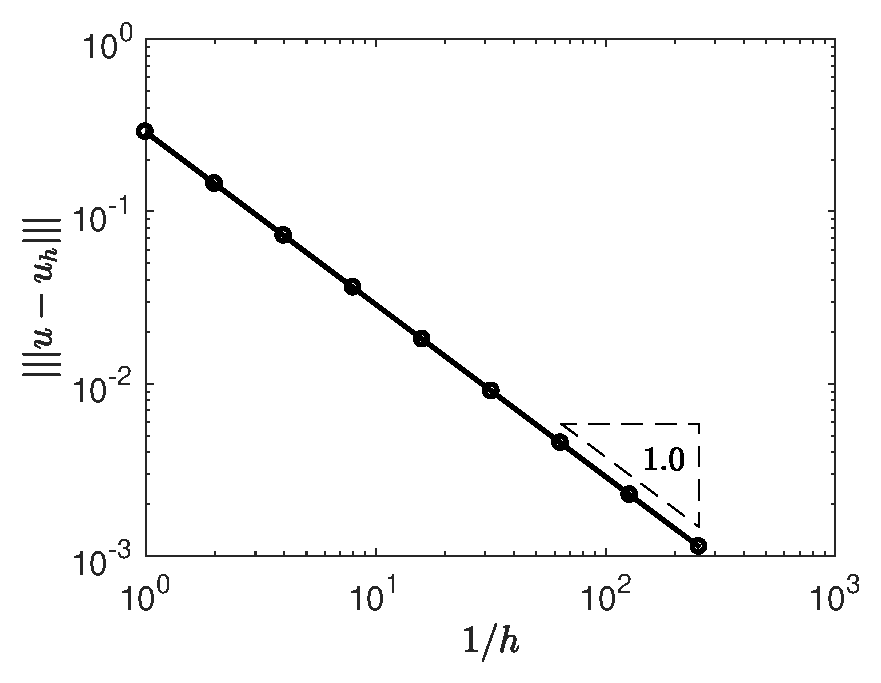
\includegraphics[width=0.5\textwidth]{poisson_1d_conv}
  \caption{Convergence of the finite element approximation for $-\Delta u = 1$.}
  \label{fig:poisson_1d_conv}
\end{figure}

\section{Summary}
In this lecture, we considered the variational formulation and the associated finite element approximation of one-dimensional Poisson equation to introduce main ideas without complexities associated with higher dimensions and more general equations.  We summarize key points of the lecture:
\begin{enumerate}
\item A one-dimensional Poisson problem can be written in the strong form, minimization form, or variational (or weak) form. 
\item The solution to the strong form is also the solution to the minimization and variational form, but the converse is not true in general.  The minimization and variational forms admit more general loads $f$ and the associated solutions.
\item A finite element approximation space $\calV_h$ is a subspace of $\calV$.  In one dimension, we may choose $\calV_h$ as the space of piecewise linear polynomials associated with a tessellation of $\Omega \subset \RR^1$ into segments.
\item The finite element solution is the solution of the minimization or variational problem in the finite element subspace $\calV_h \subset \calV$.
\item Given a basis for $\calV_h$, the finite element solution can be computed in a systematic manner by assembling the associated stiffness matrix and the load vector and by solving the linear system.
\item For the Poisson equation, the finite element approximation $u_h$ is optimal in energy norm; even \emph{if} we knew the exact solution $u \in \calV$, we could not have found a better solution in $\calV_h$ than $u_h$.
\item The error in the linear finite element approximation of the Poisson equation converges as $h^1$ in energy norm, where $h$ is the mesh spacing.
\end{enumerate}

\chapter{Variational formulation}
\label{ch:var_form}
\disclaimer

\section{Introduction}
In the previous lecture, we developed the variational formulation and the associated finite element approximation for the one-dimensional Poisson equation with homogeneous Dirichlet boundary conditions. In this lecture, we focus on the derivation of the variational formulation for problems (i) in higher spatial dimensions, (ii) with more general boundary conditions, and (iii) governed by more general equations.  In addition, we discuss the well-posedness of the variational formulation.

\section{Hilbert and Banach spaces}
We start the section with an apology: it may be difficult to appreciate the formalism provided in this section and the next two at this point.  But, we introduce these spaces upfront such that we can state our weak formulations in a proper functional setting.  We will later see that this formalism allows us to provide various theoretical results about the weak formulation and the associated finite element approximation; this strong theoretical foundation is a strength of the finite element method. 

The solutions to the PDEs are most naturally sought in Hilbert spaces. By way of preliminaries, we recall the definition of a \emph{linear space}, \emph{norm}, and \emph{inner product}. (We limit ourselves to spaces of real-valued functions; however the following statements readily extend to spaces of complex-valued functions.)
\begin{definition}[linear space]
  $\calV$ is a linear space if the following conditions hold.
  \begin{enumerate}
  \item If $w,v \in \calV$, then $w + v \in \calV$.
  \item If $w \in \calV$ and $\alpha \in \RR$, then $\alpha w \in \calV$.
  \end{enumerate}
\end{definition}
\begin{remark}
  If $\calV$ is a linear space and $v_1,\dots,v_n \in \calV$, then $\sum_{i=1}^n \alpha_i v_i \in \calV$ for any $\alpha_1, \dots, \alpha_n \in \RR$.
\end{remark}
\begin{definition}[norm]
  Given a linear space $\calV$, a norm is a function $\| \cdot \| : \calV \to \RR$ that satisfies the following three conditions: $\forall w,v \in \calV$ and $\forall \alpha \in \RR$, 
  \begin{enumerate}
  \item absolute scalability: $\| \alpha v \| = |\alpha| \| v \|$
  \item positive definiteness: $ \| v \| \geq 0$,  and $\| v \| = 0 \Leftrightarrow v = 0$
  \item triangle inequality: $  \| w + v \| \leq \| w \| + \| v \| $
  \end{enumerate}
\end{definition}
\begin{definition}[inner product]
  Given a linear space $\calV$, an inner product is a function $(\cdot,\cdot): \calV \times \calV \to \RR$ that satisfies the following three conditions: $\forall w,v,z \in \calV$ and $\forall \alpha,\beta \in \RR$,
\begin{enumerate}
\item symmetry: $(w,v) = (v,w)$
\item linearity in first argument: $ (\alpha w + \beta v, z) = \alpha (w,z) + \beta (v,z)$
\item positive definiteness: $ (v,v) \geq 0$, and $(v,v) = 0 \Leftrightarrow v = 0 $
\end{enumerate}
Note: the combination of the first and second conditions implies that the inner product is also linear in the second argument.
\end{definition}
\begin{definition}[induced norm]
  Given a linear space $\calV$ and an inner product $(\cdot,\cdot): \calV \times \calV \to \RR$, the induced norm $\| \cdot \|$ is given by
  \begin{equation*}
    \| v \| \equiv \sqrt{(v,v)} \quad \forall v \in \calV.
  \end{equation*}
\end{definition}
\begin{remark}[induced norm]
  The induced norm is a norm.
  \begin{proof}
     The absolute scalability follows from linearity:
     \begin{equation*}
       \| \alpha v \|^2 = (\alpha v, \alpha v) = \alpha^2 (v,v) = |\alpha|^2 \| v \|^2.
     \end{equation*}
     The positive definiteness of the induced norm is a direct consequence of the positive definiteness of the associated inner product.  The triangle inequality is proved using the Cauchy-Schwarz inequality in Proposition~\ref{prop:posnd_cauchy_schwarz}: $\forall w,v \in \calV$, 
     \begin{equation*}
       \| w + v \|^2
       = (w + v, w+ v)
       = \| w \|^2 + 2(w,v) + \| v \|^2
       \leq \| w \|^2 + 2 \| w \| \| v \| + \| v \|^2
       =  (\| w \| + \| v \|)^2
     \end{equation*}
     and hence $\| w + v \| \leq \| w \| + \| v \|$.
  \end{proof}
\end{remark}
\begin{proposition}[Cauchy-Schwarz inequality]
  \label{prop:posnd_cauchy_schwarz}
  Given a linear space $\calV$ and an inner product $(\cdot, \cdot): \calV \times \calV \to \RR$, the associated induced norm $\| \cdot \|: \calV \to \RR$ satisfies
  \begin{equation*}
    (w,v) \leq \| w \| \| v \| \quad \forall w ,v \in \calV.
  \end{equation*}
  \begin{proof}
    For $\|v\|=0$, the proof is trivial.  For $\| v \| \neq 0$, we observe
    \begin{equation*}
      0 \leq \left\| w - \frac{(w,v)}{\| v \|^2} v \right\|^2
      = \| w \|^2 - 2 \frac{(w,v)^2}{\| v \|^2} + \frac{(w,v)^2}{\| v \|^2}
      = \| w \|^2 - \frac{(w,v)^2}{\| v \|^2};
    \end{equation*}
    the multiplication by $\| v \|^2$ yields $(w,v)^2 \leq \| w \|^2 \| v \|^2$ or, equivalently, $(w,v) \leq \| w \| \| v \|$.
  \end{proof}
\end{proposition}

We now define a \emph{Hilbert space} and a \emph{Banach space}.
\begin{definition}[Hilbert space]
  A Hilbert space $\calV$ is a complete linear space endowed with an inner product $(\cdot,\cdot): \calV \times \calV \to \RR$ and the associated induced norm $\| \cdot \|: \calV \to \RR$ 
\end{definition}
\begin{definition}[Banach space]
  A Banach space $\calV$ is a complete linear space endowed with a norm $\| \cdot \|: \calV \to \RR$.
\end{definition}
A space $\calV$ is said to be \emph{complete} if any Cauchy sequence with respect to the norm $\| \cdot \|: \calV \to \RR$ converges to an element of $\calV$.  A sequence $v_1$, $v_2$, $v_3$, $\dots$ is said to be a Cauchy sequence if for any $\delta > 0$ there exists a number $N$ such that $\| v_i - v_j \| \leq \delta$, $\forall i,j  > N$.  Moreover, the sequence $v_i$ is said to converge to $v$ if $\| v - v_i \| \to 0$ as $i \to \infty$. The readers unfamiliar with the concept of completeness may think of a Hilbert space and a Banach space simply as an inner product space and a normed space. However, completeness is an important property of the Hilbert and Banach spaces, which makes the spaces suitable for the weak formulation of PDEs.

\section{Sobolev spaces: $L^2(\Omega)$, $H^1(\Omega)$, and $H^1_0(\Omega)$}
\label{sec:posnd_sobolev}
We now introduce some of the Hilbert spaces that are most commonly used in the weak formulation of PDEs. To begin, we characterize the domain $\Omega$ with which the function spaces are associated.
\begin{definition}[Lipschitz domain]
  A domain $\Omega \subset \RR^d$ is called a Lipschitz domain if its boundary $\partial \Omega$ is Lipschitz continuous: corners are permitted, but cusps are not.
\end{definition}
In words, Lipschitz domains are domains with a sufficient regular boundary. We will work exclusively with Lipschitz domains in this lecture.

We now introduce a space of square integrable functions on $\Omega \subset \RR^d$ (in the Lebesgue sense).
\begin{definition}[$L^2(\Omega)$ space]
  The Lebesgue space $L^2(\Omega)$ is endowed with an inner product
  \begin{equation*}
    (w,v)_{L^2(\Omega)} \equiv \int_\Omega w v dx
  \end{equation*}
  and the associated induced norm $\| w \|_{L^2(\Omega)} \equiv \sqrt{(w,w)_{L^2(\Omega)}}$; the space consists of functions
  \begin{equation*}
    L^2(\Omega) \equiv \{ w \ | \ \| w \|_{L^2(\Omega)} < \infty \}.
  \end{equation*}
\end{definition}
The $L^2(\Omega)$ space contains functions that are square integrable over $\Omega$, including functions that are discontinuous and also unbounded.  For example, consider $x^{-1/4}$ over $\Omega \equiv (0,1)$; the function is unbounded at $x = 0$ but is square integrable and hence is in $L^2(\Omega)$.   Two functions in $L^2(\Omega)$ which differ over a set of measure zero --- any points in $\RR^1$, curves in $\RR^2$, and surfaces in $\RR^3$ --- are deemed equivalent. For instance, consider two functions on $\Omega \equiv (-1,1)$,
\begin{equation*}
  f(x) \equiv \begin{cases}
    -1, \quad x \leq 0 \\
    1, \quad x > 0
  \end{cases}
  \qquad \text{and} \qquad
  g(x) \equiv \begin{cases}
    -1, \quad x < 0 \\
    1, \quad x \geq 0
  \end{cases}.
\end{equation*}
These two functions are equivalent in $L^2(\Omega)$.  (We also readily confirm that each function is square integrable.) More formally, the $L^2(\Omega)$ norm of the difference in the two functions is zero; we appeal to the properties of the Lebesgue integration --- we can omit any point (or more generally a set of measure zero) --- to obtain
\begin{equation*}
  \| f - g \|^2_{L^2(\Omega)} \equiv \int_{-1}^1 (f - g)^2 dx =
  \lim_{\epsilon \to 0}
  (\int_{-1}^{-\epsilon} (\underbrace{f - g}_{=0})^2 dx + \int_{\epsilon}^{1} (\underbrace{f - g}_{=0})^2 dx )
  =0.
\end{equation*}
Since $\| f - g \|_{L^2(\Omega)} = 0$,  $f$ and $g$ are equivalent in $L^2(\Omega)$.

\begin{definition}[weak derivative in $\RR^1$]
  Let $\Omega \subset \RR^1$ be a bounded domain and $C^\infty_0(\Omega)$ be the space of infinitely differentiable functions over $\Omega$ whose values and all derivatives are zero at the endpoints. The weak first derivative of a function $g$, $D^1g$, exists if there exists $D^1g \in L^2(\Omega)$ such that
\begin{equation*}
  \int_\Omega v D^1 g dx = - \int_\Omega \dd{v}{x} g dx \quad \forall v \in C^\infty_0(\Omega).
\end{equation*}
More generally, the weak $k$-th derivative of a function $g$, $D^kg$, exists if there exists $D^kg \in L^2(\Omega)$ such that
\begin{equation*}
  \int_\Omega v D^k g dx = (-1)^k \int_\Omega \dd{^kv}{x^k} g dx \quad \forall v \in C^\infty_0(\Omega).
\end{equation*}
\end{definition}

To make the idea of weak derivative concrete, consider the absolute-value function $g(x) = |x|$ over $\Omega \equiv (-1,1)$.  The function is not differentiable in the classical sense due to the presence of the kink.  However, we can readily show that the weak first derivative of $g$, $D^1g \in L^2(\Omega)$, exists.  We wish to find $D^1 g \in L^2(\Omega)$ such that, $\forall v \in C^\infty_0(\Omega)$, 
\begin{align*}
  \int_{-1}^1 v D^1 g dx
  &=
  - \int_{-1}^1 \dd{v}{x} g dx
  =
  - \lim_{\epsilon \to 0} ( \int_{-1}^{-\epsilon} \dd{v}{x} g dx
  + \int_{\epsilon}^1 \dd{v}{x} g dx )
  \\
  &=
  - \lim_{\epsilon \to 0} (-\int_{-1}^{-\epsilon} v \underbrace{ \dd{g}{x} }_{-1}dx + \underbrace{[vg]_{x=-1}^{-\epsilon}}_{v(-\epsilon)g(-\epsilon)}
  - \int_{\epsilon}^1 v \underbrace{ \dd{g}{x} }_{1} dx + \underbrace{[vg]_{x=\epsilon}^1}_{-v(\epsilon)g(\epsilon)} )
  \\
  &=
   \int_{-1}^{0} -1 v  dx +  \int_{0}^1 1 v dx;  %+ v(-\epsilon) g(-\epsilon) - v(\epsilon) g(\epsilon) )
%  =
% \int_{-1}^1 v H dx
\end{align*}
we observe that 
\begin{equation*}
  (D^1 g)(x) = \begin{cases}
    -1, \quad x \leq 0 \\
    1, \quad x > 0
  \end{cases}
\end{equation*}
satisfies the relationship. (The particular value at $x = 0$ is irrelevant because it is a set of measure zero.) However, the weak second derivative of $g$, $D^2g$, does not exist. To see this, we observe that
\begin{align*}
  \int_{-1}^1 v D^2 g dx
  =
  \int_{-1}^1 \dd{^2v}{x^2} g dx
  =
  \int_{-1}^0 -1 \dd{v}{x} dx + \int_{0}^1 1 \dd{v}{x} dx
  =
  [-v]_{x=-1}^0 + [v]_{x=0}^1
  =
  -2v(0).
\end{align*}
There is no function $D^2g \in L^2(\Omega)$ for which the above relationship holds.  (Note that the Dirac delta is not in $L^2(\Omega)$.)  %From hereon, we interpret any derivative $\dd{v}{x}$ in the weak sense.

%We might conclude that $(D^2 g)(x) = - 2\delta(x)$, where $\delta$ is the Dirac delta, satisfies the relationship; however, the Dirac delta is not integrable and hence is not in $L^2(\Omega)$.

We now generalize the weak derivative to functions in $\RR^d$, $d > 1$.
\begin{definition}[weak derivative in $\RR^d$]
  Let $\Omega \subset \RR^d$ and $C_0^\infty(\Omega)$ be the space of infinitely differentiable functions over $\Omega$ that vanish on the boundary $\partial \Omega$. The weak partial derivative of $g$, $\pp{g}{x_i}$, exists if there exists $\pp{g}{x_i} \in L^2(\Omega)$ such that
  \begin{equation*}
    \int_\Omega v \pp{g}{x_i} dx = - \int_\Omega \pp{v}{x_i} g dx \quad \forall v \in C_0^\infty(\Omega), \quad i = 1,\dots, d.
  \end{equation*}
  The associated gradient is $\nabla v \equiv (\pp{v}{x_1}, \dots, \pp{v}{x_d}) \in (L^2(\Omega))^d$.
\end{definition}
Having defined the weak derivative, we now define the $H^1(\Omega)$ space:
\begin{definition}[$H^1(\Omega)$ space]
  The Sobolev space $H^1(\Omega)$ is endowed with an inner product
  \begin{equation*}
    (w,v)_{H^1(\Omega)} \equiv \int_{\Omega} (\nabla v \cdot \nabla w + v w) dx
    = (\nabla v, \nabla w)_{L^2(\Omega)} + (v,w)_{L^2(\Omega)},
  \end{equation*}
  and the associated induced norm $\| w \|_{H^1(\Omega)} \equiv \sqrt{(w,w)_{H^1(\Omega)}}$; the space consists of functions
  \begin{equation*}
    H^1(\Omega) \equiv \{ w \ | \ \| w \|_{H^1(\Omega)} < \infty \}.
  \end{equation*}
\end{definition}
In words, the $H^1(\Omega)$ space consists of functions that are square integrable and whose weak first derivative is square integrable (i.e., the weak first derivative is in $L^2(\Omega)$).    For instance, the absolute-value function $g(x) = |x|$ on $\Omega \equiv (-1,1)$ is in $H^1(\Omega)$ because the function is square integrable and its weak derivative --- which is a Heaviside-like function as shown earlier --- is square integrable. On the other hand, the Heaviside-like function is not in $H^1(\Omega)$ because its weak first derivative does not exist. In general, $H^1(\Omega) \subset L^2(\Omega)$ because $H^1(\Omega)$ functions must have a square-integrable weak first derivative whereas $L^2(\Omega)$ functions do not.

Another related space that is frequently encountered in the weak formulation of PDEs is the $H^1_0(\Omega)$ space.
\begin{definition}[$H^1_0(\Omega)$ space] The $H^1_0(\Omega)$ is endowed with the $H^1(\Omega)$ inner product $(w,v)_{H^1(\Omega)} \equiv \int_\Omega (\nabla v \cdot \nabla w + v w) dx$ and consists of functions
\begin{equation*}
  H^1_0(\Omega) \equiv \{ w \in H^1(\Omega) \ | \ w|_{\partial \Omega} = 0 \},
\end{equation*}
where $\partial \Omega$ denotes the boundary of $\Omega$.
\end{definition}
The $H^1_0(\Omega)$ space consists of a subset of $H^1(\Omega)$ functions that vanish on the boundary.  Note that $H^1_0(\Omega)$ for $\Omega \equiv (0,1) \subset \RR^1$ is precisely the space $\calV$ we used in Sections~\eqref{sec:pos1d_var}~and~\eqref{sec:pos1d_min} for the variational and minimization formulations, respectively, of the one-dimensional Poisson equation with the homogeneous Dirichlet boundary conditions.  By construction $H^1_0(\Omega) \subset H^1(\Omega)$ since the $H^1(\Omega)$ space contains functions that do not vanish on the boundary.

We also introduce the $H^1(\Omega)$ \emph{semi-norm}:
\begin{definition}[$H^1(\Omega)$ semi-norm]
  The $H^1(\Omega)$ semi-norm is denoted by $| \cdot |_{H^1(\Omega)}$ and is given by
  \begin{equation*}
    | v |_{H^1(\Omega)} \equiv \left(\int_{\Omega} \nabla v \cdot \nabla v dx \right)^{1/2} = \| \nabla v \|_{L^2(\Omega)}   \quad \forall v \in H^1(\Omega).
  \end{equation*}  
\end{definition}
%\begin{remark}
  The $H^1(\Omega)$ semi-norm is not a norm on $H^1(\Omega)$.  Specifically, a semi-norm in general does not satisfy the positive definiteness condition.  For example, consider a function $v = 1$ on $\Omega \equiv (-1,1)$; the function is clearly not zero, but $|v|_{H^1(\Omega)} = \int_\Omega (\dd{v}{x})^2 dx = \int_\Omega 0 dx = 0$.
%\end{remark}

\section{Sobolev spaces: more general spaces}
While we most frequently use Sobolev spaces $L^2(\Omega)$, $H^1(\Omega)$, and $H^1_0(\Omega)$ in weak formulations of second-order PDEs, more general Sobolev spaces are required for higher-order PDEs.  We here introduce these more general spaces for completeness.  As the results below can be considered a generalization of the particular results in Section~\ref{sec:posnd_sobolev}, we will simply state them.
\begin{definition}[multi-dimensional derivative]
  Let $\alpha \equiv (\alpha_1, \dots, \alpha_d)$ be a $d$-dimensional multi-index of non-negative integers, and define its absolute value by $|\alpha| \equiv \alpha_1 + \cdots + \alpha_d$. The partial derivative operator $D^\alpha$ is given by 
  \begin{equation*}
    D^\alpha (\cdot)  \equiv \pp{^{|\alpha|} (\cdot)}{x_1^{\alpha_1}  \cdots \partial x_d^{\alpha_d}}.
  \end{equation*}
\end{definition}
\begin{definition}[$H^k(\Omega)$ space]
  For a non-negative integer $k$, the Sobolev space $H^k(\Omega)$ is endowed with an inner product
  \begin{equation*}
    (w,v)_{H^k(\Omega)} \equiv \sum_{|\alpha| \leq k} (D^\alpha w, D^\alpha v)_{L^2(\Omega)}
  \end{equation*}
  and the associated induced norm $\| w \|_{H^k(\Omega)} \equiv \sqrt{(w,w)_{H^k(\Omega)}}$; the space consists of functions
  \begin{equation*}
    H^k(\Omega) \equiv \{ w \ | \ \| w \|_{H^k(\Omega)} < \infty \}.
  \end{equation*}
\end{definition} 
\begin{definition}[$H^k(\Omega)$ semi-norm]
  The $H^k(\Omega)$ semi-norm is denoted by $| \cdot |_{H^k(\Omega)}$ and is given by
  \begin{equation*}
    | v |_{H^k(\Omega)} \equiv \| D^\alpha v \|_{L^2(\Omega)} \quad \forall v \in H^k(\Omega).
  \end{equation*}  
\end{definition}
%We finally introduce more general Banach spaces $L^p(\Omega)$ and $W^{k,p}(\Omega)$ for completeness.
\begin{definition}[$L^p(\Omega)$ space]
  The Banach space $L^p(\Omega)$ is endowed with a norm
  \begin{equation*}
    \| w \|_{L^p(\Omega)} \equiv \left(\int_\Omega |w|^p dx\right)^{1/p}
  \end{equation*}
  in the case $1 \geq p < \infty$ and
  \begin{equation*}
    \| w \|_{L^\infty(\Omega)} \equiv \esssup_{x \in \Omega} | w(x) | 
  \end{equation*}
  in the case $p = \infty$.   In either case, the $L^p(\Omega)$ space consists of functions
  \begin{equation*}
    L^p(\Omega) \equiv \{ w \ | \ \| w \|_{L^p(\Omega)} < \infty \}.
  \end{equation*}
\end{definition}
\begin{definition}[$W^k_p$ space]
  The Sobolev space $W^k_p$ is endowed with a norm
  \begin{equation*}
    \| w \|_{W^k_p(\Omega)} \equiv \left( \sum_{|\alpha|\leq k} \| D^\alpha w \|^p_{L^p(\Omega)} \right)^{1/p}
  \end{equation*}
  in the case $1 \geq p < \infty$ and
  \begin{equation*}
    \| w \|_{W^k_\infty(\Omega)} \equiv \max_{|\alpha| \leq k} \| D^\alpha w \|_{L^\infty(\Omega)}
  \end{equation*}
  in the case $p = \infty$. In either case, the $W^k_p(\Omega)$ space consists of functions
  \begin{equation*}
    W^k_p(\Omega) = \{ w \ | \| w \|_{W^k_p(\Omega)} < \infty \}.
  \end{equation*}
\end{definition}
\begin{remark}
  The $H^k(\Omega)$ space is a special case of $W^k_p(\Omega)$ space for $p = 2$.
\end{remark}

%It may be difficult to appreciate the formalism provided in this section at this point.  But, we introduce these spaces upfront such that we can state our weak formulation in a proper functional setting.  We will later see that this formalism allows us to provide various theoretical results on the weak formulation and the associated finite element approximation, which is the strength of the finite element method.



\section{$d$-dimensional Poisson problem: homogeneous Dirichlet BC}
\label{sec:posnd_homo_dir}
We consider a Poisson equation in $\RR^d$ for $d \geq 1$.  To this end, we first introduce a $d$-dimensional Lipschitz domain $\Omega \subset \RR^d$. The strong form of the Poisson equation with homogeneous Dirichlet boundary conditions is as follows: find $u$ such that
\begin{align}
  - \Delta u &= f \quad \text{in } \Omega \label{eq:posnd_strong} \\
  u &= 0 \quad \text{on } \partial \Omega \notag.
\end{align}
 Here, the Laplacian operator $\Delta$ satisfies $\Delta w \equiv \pp{^2w}{x^2_1} + \cdots + \pp{^2w}{x^2_d}$ for any $w$.  The Poisson equation models, for instance, steady heat transfer, where $u$ is the temperature field (relative to the ambient temperature), $f$ is the volume heat source, and the homogeneous Dirichlet boundary condition corresponds to the fixed-temperature condition.

The variational formulation of~\eqref{eq:posnd_strong} requires an appropriate choice of a function space.  For homogeneous Dirichlet boundary condition, the appropriate Sobolev space is
\begin{equation*}
  \calV \equiv H^1_0(\Omega).
\end{equation*}
We recall that $H^1_0(\Omega) \equiv \{ w \in H^1(\Omega) \ | \ w|_{\partial \Omega} = 0 \}$; i.e., the space consists of functions (i) whose value and first derivative are square integrable and (ii) that vanish on the boundary.  Note that any function $w \in H^1_0(\Omega)$ satisfies the boundary condition $u|_{\partial \Omega} = 0$ by construction.

To obtain a variational (or weak) form, we employ the weighted residual method: we multiply~\eqref{eq:posnd_strong} by a test function $v \in \calV$, integrate the expression, and then integrate by parts the left hand side:
\begin{equation*}
  \int_\Omega v (-\Delta u) dx = \int_\Omega v f dx \quad \Rightarrow \quad
  \int_\Omega \nabla v \cdot \nabla u dx - \underbrace{ \int_{\partial \Omega} v \pp{u}{n} ds}_{ = 0}  = \int_\Omega v f dx;
\end{equation*}
the boundary term vanishes because $v|_{\partial \Omega} = 0$ for $v \in \calV \equiv H^1_0(\Omega)$.  We now recognize the bilinear form $a: \calV \times \calV \to \RR$,
\begin{equation*}
  a(w,v) \equiv \int_\Omega \nabla v \cdot \nabla w dx \quad \forall w,v \in \calV,
\end{equation*}
and the linear form $\ell: \calV \to \RR$,
\begin{equation*}
  \ell(v) \equiv \int_\Omega v f dx \quad \forall v \in \calV.
\end{equation*}
Our variational problem is as follows: find $u \in \calV$ such that
\begin{equation}
  a(u,v) = \ell(v) \quad \forall v \in \calV. \label{eq:posnd_weak}
\end{equation}
 Using exactly the same procedure as the one-dimensional case shown in Section~\ref{sec:pos1d_var}, we can show that the solution to the strong form~\eqref{eq:posnd_strong} satisfies the variational form~\eqref{eq:posnd_weak}.  However the converse is not true in general; the variational form admits more general loads $f$ and hence solutions than the strong form.

%% For Poisson equation, which has an intrinsic energy, we can also provide a minimization form.  To this end, we introduce a functional $J: \calV \to \RR$ given by
%% \begin{equation*}
%%   J(w) \equiv \frac{1}{2} \int_\Omega \nabla w \cdot \nabla w dx - \int_\Omega f s dx \quad \forall w \in \calV.
%% \end{equation*}
%% Our minimization problem is as follows: find $u \in \calV$ such that
%% \begin{equation}
%%   u = \argmin_{w \in \calV} J(w). \label{eq:posnd_min}
%% \end{equation}
%% Again, using the same procedure as the one-dimensional case, we can show that $u \in \calV$ is the solution to the variational form~\eqref{eq:posnd_weak} if and only if it is the solution to the minimization form~\eqref{eq:posnd_min}.

\section{Mixed problems: essential and natural boundary conditions}
\label{sec:posnd_mixed}
We have so far considered Poisson equations with a homogeneous Dirichlet boundary condition.  We now consider a problem with a mixed boundary condition. To this end, given $\Omega \subset \RR^d$, we first partition the domain boundary $\partial \Omega$ into a Dirichlet part $\Gamma_D$ and a Neumann part $\Gamma_N$ such that $\overline{\partial \Omega} = \overline \Gamma_D \cup \overline \Gamma_N$ and $\Gamma_N \neq \emptyset$.  We then consider the following boundary value problem: find $u$ such that
\begin{align}
  -\Delta u &= f \quad \text{in } \Omega \notag \\
  u &= 0 \quad \text{on } \Gamma_D \label{eq:posnd_mixed_bc_strong} \\
  \pp{u}{n} &= g \quad \text{on } \Gamma_N, \notag
\end{align}
where $f$ is the volume source term and $g$ is the boundary source term.  In the case of a steady heat transfer, $f$ and $g$ represent volume and boundary heat sources, respectively.

To obtain a variational form of~\eqref{eq:posnd_mixed_bc_strong},  we redefine the function space relative to the homogeneous Dirichlet boundary condition case.  The function space suitable for the mixed boundary condition case is
\begin{equation}
  \calV \equiv \{ v \in H^1(\Omega) \ | \ v|_{\Gamma_D} = 0 \}.
  \label{eq:posnd_mixed_bc_space}
\end{equation}
Note that $H^1_0(\Omega) \subset \calV \subset H^1(\Omega)$; functions in $H^1_0(\Omega)$ must vanish everywhere on $\partial \Omega$, functions in $\calV$ must vanish only on $\Gamma_D \subset \partial \Omega$, and functions in $H^1(\Omega)$ have no conditions on their boundary values. We now apply the weighted residual method to obtain the variational form: we multiply \eqref{eq:posnd_mixed_bc_strong} by a test function $v \in \calV$, integrate the expression, and then integrate by parts the left hand side:
\begin{equation*}
  \int_\Omega v (-\Delta u) dx = \int_\Omega v f dx
  \quad \Rightarrow \quad
  \int_\Omega \nabla v \cdot \nabla u dx
  - \underbrace{\int_{\Gamma_D} v \pp{u}{n} ds}_{= 0}
  - \int_{\Gamma_N} v \pp{u}{n} ds
  =
  \int_{\Omega} v f dx;
\end{equation*}
the boundary term on $\Gamma_D$ vanishes because $v|_{\Gamma_D} = 0$ for $v \in \calV$. On the other hand, the boundary term on $\Gamma_N$ remains; we now replace $\pp{u}{n}$ with $g$ to incorporate the boundary condition we wish to impose: $\pp{u}{n} = g$ on $\Gamma_N$. The resulting weighted residual form is
\begin{equation*}
  \int_\Omega \nabla v \cdot \nabla u dx
  =
  \int_{\Omega} v f dx
  + \int_{\Gamma_N} v g ds.
\end{equation*}
We now recognize the bilinear form $a: \calV \times \calV \to \RR$ given by
\begin{equation*}
  a(w,v) \equiv \int_\Omega \nabla v \cdot \nabla w dx \quad \forall w,v \in \calV,
\end{equation*}
and the linear form $\ell: \calV \to \RR$ given by
\begin{equation*}
  \ell(v) \equiv \int_\Omega v f dx + \int_{\Gamma_N} v g ds \quad \forall v \in \calV.
\end{equation*}
Our variational problem is as follows: find $u \in \calV$ such that
\begin{equation}
  a(u,v) = \ell(v) \quad \forall v \in \calV. \label{eq:posnd_mixed_bc_weak}
\end{equation}

We readily observe that the solution to the strong form~\eqref{eq:posnd_mixed_bc_strong} satisfies the variational form~\eqref{eq:posnd_mixed_bc_weak};  for all $v \in \calV$,
\begin{align*}
  a(u,v) - \ell(v)
  &\equiv \int_\Omega \nabla v \cdot \nabla u dx - \int_\Omega vf dx - \int_{\Gamma_N} vg ds
  \\
  &= \int_\Omega v (-\Delta u) dx + \int_{\Gamma_D} v \pp{u}{n} ds + \int_{\Gamma_N} v \pp{u}{n} ds  - \int_\Omega vf dx - \int_{\Gamma_N} vg ds
  \\
  &= \int_\Omega v \underbrace{ (-\Delta u - f) }_{= 0 \text{ as $-\Delta u=  f$ in $\Omega$}} dx
  + \underbrace{ \int_{\Gamma_D} v \pp{u}{n} ds }_{= 0 \text{ as $v|_{\Gamma_D} = 0$}}
  + \int_{\Gamma_N} v \underbrace{ \left( \pp{u}{n} - g \right) }_{= 0 \text{ as $\pp{u}{n} = g$ on $\Gamma_N$}}ds = 0.
\end{align*}
Hence a solution to the strong form~\eqref{eq:posnd_mixed_bc_strong} is a solution to the variational form~\eqref{eq:posnd_mixed_bc_weak}; however, again the converse is not true as the variational form admits more general forms of $f$ and $g$ than the strong form.

In the variational formulation of the mixed boundary condition, the Dirichlet and Neumann conditions are treated differently.  On one hand, we explicitly impose the Dirichlet boundary condition $u = 0$ on $\Gamma_D$ through the choice of the space $\calV$ in~\eqref{eq:posnd_mixed_bc_space}. On the other hand, the Neumann boundary condition $\pp{u}{n} = g$ on $\Gamma_N$ is implicitly contained in the variational statement~\eqref{eq:posnd_mixed_bc_weak}.  A boundary condition that is explicitly imposed by the choice of the function space is called an \emph{essential boundary condition}; a boundary condition that is implicitly imposed by the variational statement is called a \emph{natural boundary condition}.  In the above treatment of the Poisson equation with a mixed boundary condition, the Dirichlet condition is an essential boundary condition, and the Neumann condition is a natural boundary condition.



%% We can similarly consider a minimization form of~\eqref{eq:posnd_mixed_bc_strong}.  We again work with the space $\calV \equiv \{ v \in H^1(\Omega) \ | \ v|_{\Gamma_D} = 0 \}$.  We then introduce a functional $J: \calV \to \RR$ given by
%% \begin{equation}
%%   J(w) \equiv \frac{1}{2} \int_\Omega \nabla w \cdot \nabla w dx - \int_\Omega f w dx - \int_{\Gamma_N} g w ds \quad \forall w \in \calV;
%%   \label{eq:posnd_mixed_bc_min_func}
%% \end{equation}
%% note the addition of the term on $\Gamma_N$.
%% Our minimization problem is as follows: find $u \in \calV$ such that
%% \begin{equation}
%%   u = \argmin_{w \in \calV} J(w). \label{eq:posnd_mixed_bc_min}
%% \end{equation}
%% We can readily show, using the same procedure used in Section~\ref{sec:pos1d_min}, that $u \in \calV$ is the solution to the variational problem~\eqref{eq:posnd_mixed_bc_weak} if and only if it is the solution to the minimization problem~\eqref{eq:posnd_mixed_bc_min}.

%% We can readily show that the solution to the strong form~\eqref{eq:posnd_mixed_bc_strong} satisfies the minimization condition~\eqref{eq:posnd_mixed_bc_min}. To see this, let $w = u + v$, where $u \in \calV$ is the solution to~\eqref{eq:posnd_mixed_bc_strong} and $v$ is an arbitrary function in $\calV$. We  then observe
%% \begin{align*}
%%   J(u + v)
%%   &=
%%   \frac{1}{2} \int_\Omega \nabla (u + v) \cdot \nabla (u+v) dx - \int_\Omega f (u+v) dx - \int_{\Gamma_N} g (u + v) ds
%%   \\
%%   &= \underbrace{ \frac{1}{2} \int_\Omega \nabla u \cdot \nabla u dx - \int_\Omega fu dx - \int_{\Gamma_N} g u ds }_{J(u)}
%%   \\
%%   &\quad + \underbrace{\int_{\Omega} \nabla v \cdot \nabla u dx - \int_\Omega f v - \int_{\Gamma_N} g v ds}_{J'(u;v) \text{ --- first variation}}
%%   + \underbrace{  \frac{1}{2} \int_{\Omega} \nabla v \cdot \nabla v dx }_{> 0 \text{ for } v \neq 0}.
%% \end{align*}
%% We integrate by parts the first term of $J'(u;v)$ to obtain
%% \begin{align*}
%%   J'(u;v) &= \int_{\Omega} \nabla v \cdot \nabla u dx - \int_\Omega f v dx - \int_{\Gamma_N} g v ds
%%   \\
%%   &= - \int_\Omega v (\underbrace{ \Delta u + f }_{= 0 \text{ as } -\Delta u = f \text{ in } \Omega}) dx + \int_{\Gamma_D} \underbrace{ v \pp{u}{n} }_{=0 \text{ as } v \in \calV}ds + \int_{\Gamma_N}  v (\underbrace{ \pp{u}{n} - g }_{= 0 \text{ as } \pp{u}{n} = g \text{ on } \Gamma_N}) ds = 0;
%% \end{align*}
%% if $u$ is the solution to the strong form~\eqref{eq:posnd_mixed_bc_strong}, then $J'(u;v) = 0$ for all $v \in \calV$. It follows
%% \begin{equation*}
%%   J(u+v) = J(u) + \frac{1}{2} \int_\Omega \nabla v \cdot \nabla v dx > J(u) \quad \forall v \neq 0,
%% \end{equation*}
%% and hence the solution $u$ to strong form~\eqref{eq:posnd_mixed_bc_strong} is the minimizer of the energy functional~\eqref{eq:posnd_mixed_bc_min_func} and hence the solution to the minimization form~\eqref{eq:posnd_mixed_bc_min}.


\section{Inhomogeneous Dirichlet boundary condition}
\label{sec:posnd_inhomo_bc}
We now consider a problem with \emph{inhomogeneous} Dirichlet boundary condition.  The strong form is as follows: find $u$ such that
\begin{align}
  -\Delta u &= f \quad \text{in } \Omega \label{eq:posnd_inhomo_bc_strong} \\
  u &= u^B \quad \text{on } \Gamma_D \equiv \partial \Omega \notag
\end{align}
for some boundary function $u^B$ and source term $f$. While we here focus on the pure Dirichlet problem for simplicity, the approach in this section can be combined with the approach for mixed problems in Section~\ref{sec:posnd_mixed} to treat mixed problems with inhomogeneous Dirichlet and Neumann boundary conditions.

To obtain a variational form of~\eqref{eq:posnd_inhomo_bc_strong}, we introduce spaces
\begin{align*}
  \calV^E &\equiv \{ w \in H^1(\Omega) \ | \ w|_{\Gamma_D} = u^B \}, \\
  \calV &\equiv H^1_0(\Omega).
\end{align*}
The superscript ``E'' stands for ``essential'', as the space $\calV^E$ satisfies the essential (i.e., Dirichlet) boundary condition. Note that, for $u^B \neq 0$, $\calV^E$ is \emph{not} a linear space; for $w,v \in \calV^E$, $z = w + v \notin \calV^E$ because $z|_{\Gamma_D} = 2 u^B \neq u^B$. Rather, $\calV^E$ is an \emph{affine space}: given an arbitrary fixed element $u^E \in \calV^E$ so that $u^E|_{\Gamma_D} = u^B$, we have $\calV^E = u^E + \calV = \{ u^E + v \ | \ v \in \calV \}$. We now employ the weighted residual method: we multiply~\eqref{eq:posnd_inhomo_bc_strong} by a test function $v$ in the \emph{linear space} $\calV$ --- and not \emph{affine space} $\calV^E$ ---, integrate the expression, and integrate by parts the right hand side to obtain
\begin{equation*}
  \int_{\Omega} v(-\Delta u) dx = \int_\Omega vf dx
  \quad \Rightarrow \quad
  \int_\Omega \nabla v \cdot \nabla u dx - \underbrace{ \int_{\partial \Omega} v \pp{u}{n} ds }_{= 0}
  = \int_\Omega v f dx;
\end{equation*}
again the boundary term vanishes because $v$ is in $\calV$ (and not $\calV^E$). 
We recognize a bilinear form and a linear form
\begin{align*}
  a(w,v) &\equiv \int_\Omega \nabla v \cdot \nabla w dx \quad \forall w,v \in \calV \\
  \ell(v) &\equiv \int_\Omega vf dx \quad \forall v \in \calV.
\end{align*}
The variational problem is as follows: find $u \in \calV^E$ such that
\begin{equation}
  a(u,v) = \ell(v) \quad \forall v \in \calV.
  \label{eq:posnd_inhomo_bc_var}
\end{equation}
We note that the bilinear form and linear form are identical to the homogeneous Dirichlet boundary condition case considered in Section~\ref{sec:posnd_homo_dir}.  However, our trial space is different; the space $\calV^E$ is an affine space of functions that satisfy the inhomogeneous Dirichlet boundary condition.  As discussed in Section~\ref{sec:posnd_mixed}, a Dirichlet boundary condition is an essential boundary condition, which is explicitly imposed through the choice of the space. %ecause the inhomogeneous Dirichlet boundary condition $u = u^B$ on $\Gamma_D$ is an essential boundary condition. the test space $\calV$ is a linear space of functions that vanish on the Dirichlet boundary.

We readily observe that the solution to the strong form~\eqref{eq:posnd_inhomo_bc_strong} satisfies the variational form~\eqref{eq:posnd_inhomo_bc_var};  for all $v \in \calV$,
\begin{align*}
  a(u,v) - \ell(v)
  &\equiv \int_\Omega \nabla v \cdot \nabla u dx - \int_\Omega vf dx - \int_{\Gamma_N} vg ds
  \\
  &= \int_\Omega v (-\Delta u) dx + \int_{\partial \Omega} v \pp{u}{n} ds  - \int_\Omega vf dx 
  \\
  &= \int_\Omega v \underbrace{ (-\Delta u - f) }_{= 0 \text{ as $-\Delta u=  0$ in $\Omega$}} dx
  + \underbrace{ \int_{\partial \Omega} v \pp{u}{n} ds }_{= 0 \text{ as $v|_{\Gamma_D \equiv \partial \Omega} = 0$}}.
\end{align*}
Moreover, the boundary condition $u = u^B$ on $\Gamma_D \equiv \partial \Omega$ is satisfied because $u \in \calV^E$. 
Hence a solution to the strong form~\eqref{eq:posnd_inhomo_bc_strong} is a solution to the variational form~\eqref{eq:posnd_inhomo_bc_var}; however, again the converse is not true as the variational form admits more general solutions.

In practice, it is more convenient to reformulate the problem such that both the trial and test spaces are linear.  We first choose an arbitrary fixed function $u^E$ in $\calV^E$; the function $u^E \in \calV^E$ can be any function in $H^1(\Omega)$ that satisfies the inhomogeneous Dirichlet boundary condition so that $u^E|_{\Gamma_D} = u^B$. We then express the solution $u$ as $u = u^E + \tilde u$ for $\tilde u$ in the linear space $\calV$, and rearrange the variational form~\eqref{eq:posnd_inhomo_bc_var} as
\begin{equation*}
  a(u^E + \tilde u,v) = \ell(v) \quad \Rightarrow \quad
  a(\tilde u,v) = \ell(v) - a(u^E,v).
\end{equation*}
We now recognize the right hand side $\ell(\cdot) - a(u^E,\cdot)$ as another linear form on $\calV$ and formally introduce $\tilde \ell: \calV \to \RR$ such that
\begin{equation*}
  \tilde \ell(v) \equiv \ell(v) - a(u^E,v) \quad \forall v \in \calV.
\end{equation*}
We then consider a variational problem for $\tilde u$: find $\tilde u \in \calV$ such that
\begin{equation}
  \label{eq:posnd_inhomo_bc_var_reform}
  a(\tilde u,v) = \tilde \ell(v) \quad \forall v \in \calV.
\end{equation}
Once we find $\tilde u$, we then set $u = u^E + \tilde u$, which is in $\calV^E$. Note that $\tilde u \in \calV$ depends on our choice of $u^E \in \calV^E$ because $\tilde \ell(\cdot)$ depends on $u^E$; however, the actual solution $u = u^E + \tilde u$ is independent of the particular choice of $u^E \in \calV^E$.

%% For completeness, we also introduce the minimization form.  We introduce a functional $J: \calV^E \to \RR$ given by
%% \begin{equation}
%%   J(w) \equiv \frac{1}{2} \int_{\Omega} \nabla w \cdot \nabla w dx - \int_\Omega f w dx
%%   \label{eq:posnd_inhomo_bc_min_func}
%% \end{equation}
%% and state the minimization problem: find $u \in \calV^E$ such that
%% \begin{equation}
%%   u = \argmin_{w \in \calV^E} J(w).
%%   \label{eq:posnd_inhomo_bc_min}
%% \end{equation}
%% We can readily show, using the same procedure used in Section~\ref{sec:pos1d_min}, that $u \in \calV^E$ is the solution to the variational problem~\eqref{eq:posnd_inhomo_bc_var} if and only if it is the solution to the minimization problem~\eqref{eq:posnd_inhomo_bc_min}.

%% We now show that the solution to~\eqref{eq:posnd_inhomo_bc_strong} satisfies the minimization statement~\eqref{eq:posnd_inhomo_bc_min}. We first set $w = u + v$, where $u \in \calV^E$ is the solution to~\eqref{eq:posnd_inhomo_bc_strong} and $v$ is an arbitrary function in $\calV$ (and \emph{not} $\calV^E$). We then observe
%% \begin{align*}
%%   J(u + v)
%%   &=
%%   \frac{1}{2} \int_\Omega \nabla (u + v) \cdot \nabla (u+v) dx - \int_\Omega f (u+v) dx 
%%   \\
%%   &= \underbrace{ \frac{1}{2} \int_\Omega \nabla u \cdot \nabla u dx - \int_\Omega fu dx }_{J(u)}
%%   + \underbrace{\int_{\Omega} \nabla v \cdot \nabla u dx - \int_\Omega f v }_{J'(u;v) \text{ --- first variation}}
%%   + \underbrace{  \frac{1}{2} \int_{\Omega} \nabla v \cdot \nabla v dx }_{> 0 \text{ for } v \neq 0}.
%% \end{align*}
%% We integrate by parts the first term of $J'(u;v)$ to obtain
%% \begin{equation*}
%%   J'(u;v) = \int_{\Omega} \nabla v \cdot \nabla u dx - \int_\Omega f v
%%   = - \int_\Omega v (\underbrace{ \Delta u + f }_{= 0 \text{ as } -\Delta u = f \text{ in } \Omega}) dx + \int_{\Gamma_D \equiv \partial \Omega} \underbrace{ v \pp{u}{n} }_{=0 \text{ as } v \in \calV}ds  = 0;
%% \end{equation*}
%% the second term vanishes because $v \in \calV$ (and not $\calV^E$). It follows
%% \begin{equation*}
%%   J(u+v) = J(u) + \frac{1}{2} \int_\Omega \nabla v \cdot \nabla v dx > J(u) \quad \forall v \neq 0,
%% \end{equation*}
%% and hence the solution $u$ to strong form~\eqref{eq:posnd_mixed_bc_strong} is the minimizer of the functional~\eqref{eq:posnd_mixed_bc_min_func} and hence the solution to the minimization form~\eqref{eq:posnd_mixed_bc_min}.


%The solution is sought in the space $\calV^E$ that satisfies the inhomogeneous Dirichlet boundary condition, while the test functions are in the space $\calV$.



\section{General second-order elliptic equation}
We have so far considered the variational formulation of Poisson equations with various boundary conditions. We can readily extend our approach to treat general second-order elliptic equations. To demonstrate the idea, we consider a convection-reaction-diffusion equation with (inhomogeneous) Dirichlet, Neumann, and Robin boundary conditions. To this end, we partition the Lipschitz domain $\Omega \subset \RR^d$ into the Dirichlet boundary $\Gamma_D$, the Neuamnn boundary $\Gamma_N$, and the Robin boundary $\Gamma_R$ such that $\overline{\partial \Omega} = \overline{\Gamma}_D \cup \overline{\Gamma}_N \cup \overline{\Gamma}_R$; we assume $\Gamma_D \cup \Gamma_R \neq \emptyset$. We then consider a problem of the following form: find $u$ such that
\begin{align}
  - \nabla \cdot (a \nabla u) + b \cdot \nabla u + c u &= f \quad \text{in } \Omega
  \notag \\
  u &= u^B \quad \text{on } \Gamma_D \label{eq:posnd_gen_strong} \\
  n \cdot a \nabla u &= g \quad \text{on } \Gamma_N \notag \\
  n \cdot a \nabla u + k u &= q \quad \text{on } \Gamma_R, \notag
\end{align}
where $a: \Omega \to \RR^{d \times d}$ is the diffusivity tensor, $b: \Omega \to \RR^d$ is the advection vector, $c: \Omega \to \RR$ is the reaction constant, $f: \Omega \to \RR$ is the source term,  $n: \partial \Omega \to \RR^d$ is the outward-point normal on $\partial \Omega$, $u^B: \Gamma_D \to \RR$ is the Dirichlet boundary function, $g: \Gamma_N \to \RR$ is the Neumann source term, $k: \Gamma_R \to \RR$ is the Robin coefficient, and $q: \Gamma_R \to \RR$ is the Robin source term.  Note that in general each coefficient is spatially varying and hence is a function of space; e.g., the diffusivity tensor evaluated at $x \in \Omega \subset \RR^d$ is in $\RR^{d \times d}$ and hence is denoted $a: \Omega \to \RR^{d \times d}$.  For the second-order PDE to be \emph{elliptic}, we require that the diffusitivity tensor is symmetric positive definite almost everywhere: $a(x) \in \RR^{d \times d}$ satisfies
\begin{equation*}
  \xi^T a(x) \xi > 0 \quad \forall \xi \neq 0 \quad \text{ a.e. in } \Omega.
%  \sum_{i,j=1}^d a_{ij}(x) \xi_i \xi_j > 0 \quad \forall \xi \in \RR^d \text{ a.e. in } \Omega.
\end{equation*}
Also note that in order for the differentiation $\nabla \cdot ( a \nabla u)$ for the \emph{strong formulation} \eqref{eq:posnd_gen_strong} to be well defined, the diffusivity tensor field must satisfy certain smoothness conditions; we will soon see that this is not a requirement for the weak formulation.

To obtain a variational form of~\eqref{eq:posnd_gen_strong}, we introduce spaces
\begin{align*}
  \calV^E &\equiv \{ w \in H^1(\Omega) \ | \ w|_{\Gamma_D} = u^B \}, \\
  \calV &\equiv \{ w \in H^1(\Omega) \ | \ w_{\Gamma_D} = 0 \}.
\end{align*}
As discussed in Section~\ref{sec:posnd_inhomo_bc}, the Dirichlet boundary condition is imposed strongly; the Neumann and Robin boundary conditions are imposed weakly.  We now multiply~\eqref{eq:posnd_gen_strong} by a test function $v$ in the linear space $\calV$, integrate the expression, and integrate by parts the diffusion term to obtain
\begin{align*}
  &\int_\Omega v (- \nabla \cdot a \nabla u + b \cdot \nabla u + c u - f) dx = 0 \\
  & \Rightarrow
  \int_\Omega (\nabla v \cdot a \nabla u  + v b \cdot \nabla u + c vu -vf ) dx
  -  \underbrace{\int_{\Gamma_D} v n \cdot a \nabla u ds}_{\text{(D)}}
  - \underbrace{\int_{\Gamma_N} v n \cdot a \nabla u ds}_{\text{(N)}}
  - \underbrace{\int_{\Gamma_R} v n \cdot a \nabla u ds}_{\text{(R)}}
\end{align*}
We now impose the boundary conditions.  The Dirichlet boundary condition is imposed strongly by the choice of the trial space $\calV^E$ and the test space $\calV$; the term (D) vanishes because $v|_{\Gamma_D} = 0$ for all $v \in \calV$.  The Neumann boundary condition $n \cdot a \nabla u = g$ is weakly imposed; we replace the boundary term (N) by $\int_{\Gamma_N} v g ds$.  The Robin boundary condition $\pp{u}{n} + k u = q$ is also weakly imposed; we replace the boundary term (R) by $\int_{\Gamma_R} v (-ku + q) ds$.  Upon the substitution of the appropriate boundary conditions, our weighted-residual formulation reads as follows: find $u \in \calV^E$ such that
\begin{equation*}
  \int_\Omega (\nabla v \cdot a \nabla u  + v b \cdot \nabla u + c vu - vf) dx
  - \int_{\Gamma_N} v g ds - \int_{\Gamma_R} v (-ku + q) ds = 0
  \quad \forall v \in \calV.
\end{equation*}
Some reorganization of the terms yield the following variational formulation: find $u \in \calV^E$ such that
\begin{equation}
  a(u,v) = \ell(v) \quad \forall v \in \calV,
  \label{eq:posnd_gen_weak}
\end{equation}
where
\begin{align*}
  a(w,v) &\equiv \int_\Omega (\nabla v \cdot a \nabla w + v b \cdot \nabla u + c vu ) dx + \int_{\Gamma_R} k vw ds \quad \forall w, v \in \calV \\
  \ell(v) &\equiv \int_\Omega fv dx + \int_{\Gamma_N} gv ds + \int_{\Gamma_R} qv ds.
  \quad \forall v \in \calV.
\end{align*}
With the variational formulation~\eqref{eq:posnd_gen_weak}, unlike with the strong formulation~\eqref{eq:posnd_gen_strong}, we need not assume any smoothness of the coefficients $a$, $b$, or $c$.  We only require that the coefficients are bounded: $a \in (L^\infty(\Omega))^{d \times d}$, $b \in (L^\infty(\Omega))^d$, and $c \in L^\infty(\Omega)$.

As discussed in Section~\ref{sec:posnd_inhomo_bc}, in practice, the inhomogeneous Dirichlet boundary conditions are more conveniently treated through the decomposition of the solution as $u = u^E + \tilde u$ for some arbitrary but fixed $u^E \in \calV^E$ so that $u^E|_{\Gamma_D} = u^B$ and $\tilde u \in \calV$.  We then consider the following variational problem: find $\tilde u \in \calV$ such that
\begin{equation*}
  a(\tilde u,v) = \tilde \ell(v) \quad \forall v \in \calV,
\end{equation*}
where $\tilde \ell: \calV \to \RR$ is the modified linear form such that $\tilde \ell(v) \equiv \ell(v) - a(u^E,v)$, $\forall v \in \calV$; we then set $u = u^E + \tilde u$. 

%% We note that it is also possible to perform the procedure in reverse: we start from the variational form and then identify the associated strong form. Specifically, we start with the variational form, and invoke the integration by parts to identify the PDE and boundary conditions: for all $v \in \calV$,
%% \begin{align*}
%%   0 &=
%%   a(u,v) - \ell(v)
%%   =
%%   \int_\Omega \nabla v \cdot \nabla u dx + \int_{\Gamma_R} k vu ds
%%   - \int_\Omega fv dx - \int_{\Gamma_N} gv ds - \int_{\Gamma_R} qv ds
%%   \\
%%   &= \int_\Omega v (-\Delta u) dx + \int_{\partial \Omega} v \pp{u}{n} ds
%%   + \int_{\Gamma_R} k vu ds
%%   - \int_\Omega fv dx - \int_{\Gamma_N} gv ds - \int_{\Gamma_R} qv ds
%%   \\
%%   &=
%%   \int_\Omega v(-\Delta u - f) dx
%%   + \underbrace{\int_{\Gamma_D} v \pp{u}{n} ds}_{=0 \text{ since $v \in \calV$}}
%%   + \int_{\Gamma_N} v (\pp{u}{n} - g) ds
%%   + \int_{\Gamma_R} v (\pp{u}{n} + ku - q) ds.
%% \end{align*}
%% In order for the statement to hold for \emph{all} $v \in \calV$, we need each of the integrals to vanish.  The condition requires that
%% \begin{align*}
%%   -\Delta u &= f \quad \text{in } \Omega \\
%%   \pp{u}{n} &= g \quad \text{on } \Gamma_N \\
%%   \pp{u}{n} + ku &= q \quad \text{on } \Gamma_R.
%% \end{align*}
%% We have identified (i) the PDE, (ii) the Neumann boundary condition on $\Gamma_N$, and (iii) the Robin boundary condition on $\Gamma_R$.  Finally, because $u \in \calV^E \equiv \{ u \in H^1(\Omega) \ | \ u|_{\Gamma_D} = u^B \}$, we have
%% \begin{equation*}
%%   u|_{\Gamma_D} = u^B \quad \text{on } \Gamma_D,
%% \end{equation*}
%% which is the Dirichlet boundary condition on $\Gamma_D$.

\section{Well-posedness of the weak formulation}
\label{sec:var_wellposedness}
We now address a fundamental question: what conditions should a weak formulation satisfy to guarantee the existence \emph{and} uniqueness of the solution?  We recall that, in general, a weak formulation is defined by a test space $\calV$, trial space $\calV^E \equiv u^E + \calV$, bilinear form $a(\cdot,\cdot)$, and linear form $\ell(\cdot)$; as such, we wish to identify conditions that these ingredients must satisfy to ensure the existence and uniqueness of the solution.

We first provide a few definitions that characterize a linear form and bilinear form.
\begin{definition}[dual norm and continuity]
  The dual norm of a linear functional $\ell \in \calV'$ is given by
  \begin{equation*}
    \| \ell \|_{\calV'} \equiv \sup_{v \in \calV} \frac{|\ell(v)|}{\| v \|_\calV}.
  \end{equation*}
  A linear functional is said to be \emph{continuous} if $\| \ell \|_{\calV'} < \infty$.
\end{definition}
\begin{corollary}
  If a linear form $\ell \in \calV'$ is continuous so that $\| \ell \|_{\calV}' < \infty$, then
  \begin{equation*}
    |\ell(v)| \leq \| \ell \|_{\calV'} \| v \|_\calV \quad \forall v \in \calV.
  \end{equation*}
  In other words, a linear form is continuous if $\exists c < \infty$ such that $| \ell(v) | \leq c \| v \|_\calV$, $\forall v \in \calV$.
\end{corollary}
\begin{definition}[continuity]
  \label{def:th_continuity}
  A bilinear form $a: \calV \times \calV \to \RR$ is said to be continuous on $\calV$ (or $\calV$-continuous) if $\exists \gamma < \infty$ such that 
  \begin{equation*}
    a(w,v) \leq \gamma \| w \|_\calV \| v \|_\calV \quad \forall w,v \in \calV,
  \end{equation*}
\end{definition}
\begin{definition}[coercivity]
  \label{def:th_coercivity}
  A bilnear form $a: \calV \times \calV \to \RR$ is said to be coercive on $\calV$ (or $\calV$-coercive) if $\exists \alpha > 0$ such that 
  \begin{equation*}
    a(v,v) \geq \alpha \| v \|_\calV^2 \quad \forall v \in \calV.
  \end{equation*}
\end{definition}
The following theorem provides an answer to the question regarding the existence and uniqueness of a weak solution.
\begin{theorem}[Lax-Milgram]
  \label{thm:lax_milgram}
  Given a Hilbert space $\calV$, a continuous, coercive bilinear form $a: \calV \times \calV \to \RR$, and a continuous linear functional $\ell \in \calV'$, there exists a unique $u \in \calV$ such that
  \begin{equation}
    a(u,v) = \ell(v) \quad \forall v \in \calV.
    \label{eq:posnd_lax_milgram}
  \end{equation}
  \begin{proof}
    The proof of existence is beyond the scope of this course.  We refer to Brenner and Scott (2008).

    The proof of uniqueness is as follows. Suppose we have two solutions $u_1 \in \calV$ and $u_2 \in \calV$ that are distinct ($u_1 \neq u_2$) and satisfy~\eqref{eq:posnd_lax_milgram}: i.e., $a(u_1,v) = \ell(v)$, $\forall v \in \calV$, and $a(u_2,v) = \ell(v)$, $\forall v \in \calV$. The subtraction of the two equations yields $a(u_1,v) - a(u_2,v) = 0$, $\forall v \in \calV$.  We then invoke bilinearity to obtain $a(u_1 - u_2,v) = 0$, $\forall v \in \calV$. We then choose $v = u_1 - u_2$, which yields $a(u_1 - u_2, u_1 - u_2) = 0$.  The coercivity of the bilinear form implies that $a(u_1 - u_2, u_1 - u_2) \geq \alpha \| u_1 - u_2 \|^2_\calV$; since the left hand side is $0$, we obtain $\| u_1 - u_2 \|^2_\calV = 0$.  Hence, we arrive at the contradiction: $u_1 = u_2$.  If two solutions satisfy~\eqref{eq:posnd_lax_milgram}, then they must be the same; the solution to~\eqref{eq:posnd_lax_milgram} is unique.
  \end{proof}
\end{theorem}
The Lax-Milgram theorem provides sufficient conditions under which a weak formulation possess a unique solution.  We however note that these are only sufficient, and not necessary, conditions.  The above proof for uniqueness also shows how certain properties of the ingredients, such as bilinearity and coercivity, are used to prove the desired result.


The Lax-Milgram theorem concerns with the existence and uniqueness of a weak solution.  We now introduce a \emph{stability} or \emph{well-posedness} result which shows that the solution $u$ depends continuously on the data $\ell(\cdot)$.
\begin{proposition}[stability]
  Suppose the conditions of the Lax-Milgram theorem, Theorem~\ref{thm:lax_milgram}, are satisfied. Then, the solution $u$ satisfies
  \begin{equation*}
    \| u \|_\calV \leq \frac{1}{\alpha} \| \ell \|_{\calV'},
  \end{equation*}
  where $\alpha$ is the coercivity constant.
  \begin{proof}
    The proof is trivial for $\| u \|_\calV = 0$. For $\| u \|_\calV \neq 0$, we appeal to the coercivity of the bilinear form and the continuity of the linear form:
    \begin{equation*}
      \alpha \| u \|_\calV^2 \leq a(u,u) = \ell(u) \leq \| \ell \|_{\calV'} \| u \|_\calV.
    \end{equation*}
    The division by $\| u \|_\calV \neq 0$ yields the desired result.
  \end{proof}
\end{proposition}
\begin{corollary}
  Suppose the conditions of the Lax-Milgram theorem, Theorem~\ref{thm:lax_milgram}, are satisfied.  In addition, consider two linear forms $\ell_1(\cdot)$ and $\ell_2(\cdot)$, and the associated solutions $u_1$ and $u_2$.  Then, the difference in the solutions, $u_1 - u_2$, is bounded by the difference in the data, $\ell_1 - \ell_2$:
  \begin{equation*}
    \| u_1 - u_2 \|_\calV \leq \frac{1}{\alpha} \| \ell_1 - \ell_2 \|_{\calV'}.
  \end{equation*}
\end{corollary}
The stability result shows that the energy norm of the solution $u$ is bounded by the dual norm of the data $\ell$.  The closely related result in the corollary can be interpreted to mean that a small disturbance in the data $\ell$ results in a small perturbation in the solution $u$.


Before we conclude this section, we remark on the well-posedness of problems with inhomogeneous Dirichlet data.  The Lax-Milgram theorem~\ref{thm:lax_milgram} requires both the test and trial spaces to be a Hilbert space and in particular linear. We however recall that the trial space for a problem with inhomogeneous Dirichlet data is an affine space $\calV^E \equiv u^E + \calV$ for some fixed $u^E \in H^1(\Omega)$ and a linear space $\calV$. To prove the existence and uniqueness of the solution, we rely on the reformulated variational formulation \eqref{eq:posnd_inhomo_bc_var_reform}, which decomposes the solution $u \in \calV^E$ as $u = u^E + \tilde u$ for an arbitrary (but fixed $u^E$) and $\tilde u \in \calV$.  We specifically apply the Lax-Milgram theorem to the problem for $\tilde u$: find $\tilde u \in \calV$ such that
  \begin{equation*}
    a(\tilde u, v) = \tilde \ell(v) \quad \forall v \in \calV,
  \end{equation*}
  where $\tilde \ell: \calV \to \RR$ is the reformulated linear form $\tilde \ell(v) \equiv \ell(v) - a(u^E,v)$, $\forall v \in \calV$. By the Lax-Milgram theorem, a unique solution to the problem exists if $a:\calV \times \calV \to \RR$ is coercive and continuous, and $\tilde \ell \in \calV'$ is continuous. The latter requires that $\exists C < \infty$ such that $|\tilde \ell(v)| \leq C\| v \|_\calV$, $\forall v \in \calV$.  We now observe that, assuming $\ell(\cdot)$ and $a(\cdot,\cdot)$ are continuous, 
  \begin{align*}
    | \tilde \ell(v) | \equiv | \ell(v) - a(u^E,v) |
    \leq | \ell(v) | + | a(u^E,v) |
    \leq c \| v \|_{\calV} + \gamma \| u^E \|_{\calV} \| v \|_{\calV}
    = (c + \gamma \| u^E \|_{\calV}) \| v \|_{\calV},
  \end{align*}
  where $c$ and $\gamma$ are the continuity constant for $\ell(\cdot)$ and $a(\cdot,\cdot)$, respectively.  Hence $\tilde \ell(\cdot)$ is continuous under these assumptions, and we can apply the Lax-Milgram theorem to show the existence and uniqueness of $\tilde u \in \calV$ and in turn $u = u^E + \tilde u \in \calV^E$.

\section{Poincar\'e-Friedrichs and trace inequalities}
The proof of existence and uniqueness of a weak solution using the Lax-Milgram theorem relies on the continuity and coercivity of the bilinear form and the continuity of the linear form.  For many bilinear forms associated with boundary value problems, the verification of coercivity relies on the Poincar\'e-Friedrichs inequality.
\begin{proposition}[Poincar\'e-Friedrichs inequality]
  \label{prop:posnd_friedrichs}
  Let $\Omega \subset \RR^d$ be a Lipschitz domain, and suppose $\Gamma \subset \partial \Omega$ and $\Gamma \neq \emptyset$. Then, there exists a constant $C_{\rm PF} < \infty$ that only depends on $\Omega$ and $\Gamma$ such that
  \begin{equation*}
    \| v \|_{L^2(\Omega)}^2 \leq C_{\rm PF} ( | v |^2_{H^1(\Omega)} + \| v \|^2_{L^2(\Gamma)} )  \quad \forall v \in H^1(\Omega).
  \end{equation*}
  \begin{proof}
    Proof of the proposition is beyond the scope of this course.  We refer to Brenner and Scott (2008).
  \end{proof}
\end{proposition}
\begin{corollary}
  \label{cor:posnd_friedrichs_1}
  Let $\Omega \subset \RR^d$ be a Lipschitz domain, and suppose $\Gamma_D \subset \partial \Omega$ and $\Gamma_D \neq \emptyset$.   Let $\calV \equiv \{ v \in H^1(\Omega) \ | \ v|_{\Gamma_D} = 0 \}$.  Then, there exists a constant $C_{\rm PF} < \infty$ that depends only on $\Omega$ and $\Gamma_D$ such that
  \begin{equation*}
    %\| v \|_{H^1(\Omega)} \leq C | v |_{H^1(\Omega)} \quad \forall v \in \calV.
    \| v \|_{L^2(\Omega)} \leq C_{\rm PF} | v |_{H^1(\Omega)} \quad \forall v \in \calV.
  \end{equation*}
\end{corollary}
\begin{corollary}
  \label{cor:posnd_friedrichs_2}
  Let $\Omega \in \RR^d$ be a Lipschitz domain. Then, there exists a constant $C_{\rm PF} < \infty$ that depends on only $\Omega$ such that
  \begin{equation*}
    \| v \|_{L^2(\Omega)} \leq C_{\rm PF} | v |_{H^1(\Omega)} \quad \forall v \in H^1_0(\Omega).
  \end{equation*}
\end{corollary}
Proposition~\ref{prop:posnd_friedrichs} allows us to bound the $L^2(\Omega)$ norm of a function by the $H^1(\Omega)$ \emph{semi}-norm of the function and the $L^2(\Gamma)$ norm of the trace of the function on a portion of the boundary, $\Gamma \subset \partial \Omega$.  Corollaries~\ref{cor:posnd_friedrichs_1}~(and~\ref{cor:posnd_friedrichs_2}) are specializations of the results for functions that vanish on a portion (and whole) of the boundary such that $\| u \|_{L^2(\Gamma_D)} = 0$.  Intuitively, the corollaries bound the (integrated) value of the function by the (integrated) gradient of the function, assuming that the function is ``pinned'' to vanish over a portion of the boundary.
%The special case of Proposition~\ref{prop:th_poincare_gen} for $\Gamma_D \equiv \partial \Omega$ is known as the \emph{Poincar\'e inequality}.
\begin{remark}[Naming of the Poincar\'e-Friedrichs inequality]
  Proposition~\ref{cor:posnd_friedrichs_1} and the related results, such as Corollaries~\ref{cor:posnd_friedrichs_1}~and~\ref{cor:posnd_friedrichs_2}, are sometimes called just Poincar\'e inequality or Friedrichs inequality.  In this note, we will refer to inequalities of these types collectively as Poincar\'e-Friedrichs inequalities.
\end{remark}

For many bilinear forms associated with boundary value problems, the verification of continuity relies on the trace inequality.
\begin{proposition}[trace inequality]
  \label{prop:posnd_trace_ineq}
  Let $\Omega \subset \RR^d$ be a Lipschitz domain. Then, there exists a constant $C_{\rm tr} < \infty$ that depends only on $\Omega$ such that
  \begin{equation*}
    \| v \|_{L^2(\partial \Omega)} \leq C_{\rm tr} \| v \|_{H^1(\Omega)} \quad \forall v \in H^1(\Omega).
  \end{equation*}
    \begin{proof}
    Proof of the proposition is beyond the scope of this course.  We refer to Brenner and Scott (2008).
  \end{proof}
\end{proposition}
The trace inequality is particularly useful when we wish to show continuity of a linear or bilinear form which involves integration over (a part of) the boundary.


\section{Example: well-posedness of a Poisson problem}
\label{eq:posnd_wellposedness_example}
We now demonstrate the application of the Lax-Milgram theorem to prove that the mixed Poisson problem considered in Section~\ref{sec:posnd_mixed} is well-posed.  The problem is reproduced here for convenience.  Let $\Omega \subset \RR^d$ be a Lipschitz domain, $\Gamma_D$ and $\Gamma_N$ be Dirichlet and Neumann boundaries such that $\overline{\partial \Omega} = \overline{\Gamma}_D \cup \overline{\Gamma}_N$ and $\Gamma_D \neq \emptyset$, and $\calV \equiv \{ v \in H^1(\Omega) \ | \ v|_{\Gamma_D} = 0 \}$.  Find $u \in \calV$ such that
\begin{equation*}
  a(u,v) = \ell(v) \quad \forall v \in \calV,
\end{equation*}
where
\begin{align*}
  a(w,v) &= \int_\Omega \nabla v \cdot \nabla w dx \quad \forall w,v \in \calV, \\
  \ell(v) &= \int_\Omega v f dx + \int_{\Gamma_N} v g ds \quad \forall v \in \calV
\end{align*}
for $f \in L^2(\Omega)$ and $g \in L^2(\Gamma_N)$.  The space $\calV$ is endowed with the standard $H^1(\Omega)$ inner product and norm; i.e., $(\cdot,\cdot)_\calV \equiv (\cdot,\cdot)_{H^1(\Omega)}$ and $\| \cdot \|_\calV \equiv \| \cdot \|_{H^1(\Omega)}$.

We first show that the bilinear form is continuous: $\forall w,v \in \calV$, 
\begin{equation*}
  a(w,v)
  =
  \int_\Omega \nabla v \cdot \nabla w dx
  \leq
  \| \nabla v \|_{L^2(\Omega)} \| \nabla w \|_{L^2(\Omega)}
  =
  | v |_{H^1(\Omega)} | w |_{H^1(\Omega)}
  \leq
  \| v \|_{H^1(\Omega)} \| w \|_{H^1(\Omega)};
\end{equation*}
here, the first inequality follows from Cauchy-Schwarz, and the last inequality follows from $| v |_{H^1(\Omega)}^2 \leq | v |_{H^1(\Omega)}^2 + \| v \|_{L^2(\Omega)}^2 \equiv \| v \|_{H^1(\Omega)}^2$.  Hence, the bilinear form is continuous with the continuity constant $C = 1$.
We next show that the bilinear form is coercive: $\forall v \in \calV$,
\begin{equation*}
  \| v \|^2_{H^1(\Omega)} = | v |^2_{H^1(\Omega)} + \| v \|^2_{L^2(\Omega)}
  \leq | v |^2_{H^1(\Omega)} + C_{\rm PF}^2 | v |^2_{H^1(\Omega)}
  = (1 + C_{\rm PF}^2) a(v,v),
\end{equation*}
where $C_{\rm PF} < \infty$ is the constant associated with the (corollary of the) Poincar\'e-Friedrichs inequality, Corollary~\ref{cor:posnd_friedrichs_1}.  It follows that $(1+C_{\rm PF}^2)^{-1}\| v \|^2_{H^1(\Omega)} \leq a(v,v)$, $\forall v \in \calV$.  Hence, the bilinear from is coercive with the coercivity constant  $\alpha = (1 + C_{\rm PF}^2)^{-1}$.  We now show that the volume source term of the linear form is continuous: $\forall v \in \calV$,
\begin{align}
  |\int_\Omega vf dx|
  \leq \| v \|_{L^2(\Omega)} \| f \|_{L^2(\Omega)}
  \leq \| f \|_{L^2(\Omega)} \| v \|_{H^1(\Omega)};
  \label{eq:posnd_example_f}
%  \| \int_{\Omega} \cdot\,f dx \|_{\calV'}
%  &\equiv \sup_{v \in \calV}
%  \frac{|\int_\Omega v f dx|}{\| v \|_{H^1(\Omega)}}
%  \leq \sup_{v \in \calV} \frac{\| v \|_{L^2(\Omega)} \| f \|_{L^2(\Omega)}}{\| v \|_{H^1(\Omega)}}
%  \leq\| f \|_{L^2(\Omega)} < \infty; %+ C_{\rm tr}\| g \|_{L^2(\Omega)}< \infty;
\end{align}
here, the first inequality follows from Cauchy-Schwarz, and the second inequality follows from $\| v\|_{L^2(\Omega)} \leq (\| v \|^2_{L^2(\Omega)} + | v |_{H^1(\Omega)}^2)^{1/2} = \| v \|_{H^1(\Omega)}^2$, $\forall v \in \calV$. We then show that the Neumann boundary term of the linear form is continuous: $\forall v \in \calV$,
\begin{align}
  |\int_{\Gamma_N} vgds|
  \leq \| v \|_{L^2(\Gamma_N)} \| g \|_{L^2(\Gamma_N)}
  \leq C_{\rm tr} \| g \|_{L^2(\Gamma_N)}  \| v \|_{H^1(\Omega)};
  \label{eq:posnd_example_g}
%  \| \int_{\Gamma_N} \cdot\,g ds \|_{\calV'}
%  &\equiv \sup_{v \in \calV}
%  \frac{|\int_{\Gamma_N} v g ds|}{\| v \|_{H^1(\Omega)}}
%  \leq \sup_{v \in \calV} \frac{ \| v \|_{L^2(\Gamma_N)} \| g \|_{L^2(\Gamma_N)}}{\| v \|_{H^1(\Omega)}}
%  \leq \sup_{v \in \calV} \frac{C_{\Omega} \| v \|_{H^1(\Omega)} \| g \|_{L^2(\Gamma_N)} }{\| v \|_{H^1(\Omega)}}
%  \\
%  &\leq C_{\Omega}\| g \|_{L^2(\Omega)}< \infty;
\end{align}
here, the first inequality follows from Cauchy-Schwarz, and the second inequality follows from the trace inequality, Proposition~\ref{prop:posnd_trace_ineq}. The combination of \eqref{eq:posnd_example_f} and \eqref{eq:posnd_example_g} yields, $\forall v \in \calV$,
\begin{equation*}
  | \ell(v) | \leq | \int_\Omega vf dx | + |\int_{\Gamma_N} vg ds|
  \leq  (\| f \|_{L^2(\Omega)} + C_{\rm tr} \| g \|_{L^2(\Gamma_N)}) \| v \|_{H^1(\Omega)};
\end{equation*}
hence the linear form $\ell(\cdot)$ is continuous with the continuity constant $c =  \| f \|_{L^2(\Omega)} + C_{\rm tr} \| g \|_{L^2(\Gamma_N)}$.  We confirm that all conditions of the Lax-Milgram theorem are satisfied; hence the Poisson problem has a unique solution, and the problem is well-posed.

\section{Minimization formulation}
We now obtain the minimization formulation for boundary value problems under two assumptions on the bilinear form $a(\cdot,\cdot)$:
\begin{itemize}
\item[1.] coercivity: $\exists \alpha > 0$ such that $a(v,v) \geq \alpha\| v \|^2_\calV$, $\forall v \in \calV$.
\item[2.] symmetry: $a(w,v) = a(v,w)$, $\forall w,v, \in \calV$.
\end{itemize}
Our variational formulation is as follows: find $u \in \calV^E$ such that
\begin{equation}
  a(u,v) = \ell(v) \quad \forall v \in \calV,
  \label{eq:posnd_energy_var}
\end{equation}
where $\calV^E \equiv  \{ v \in H^1(\Omega) \ | \ v|_{\Gamma_D} = u^B\}$ for some boundary function $u^B$, $ \calV \equiv \{ v \in H^1(\Omega) \ | \ v|_{\Gamma_D} = 0 \}$, and a continuous linear form $\ell: \calV \to \RR$.
  We then introduce an energy functional, $J: H^1(\Omega) \to \RR$, given by
\begin{equation}
  J(w) \equiv \frac{1}{2} a(w,w) - \ell(w) \quad \forall w \in H^1(\Omega).
  \label{eq:posnd_energy_fun}
\end{equation}
 We then have the following minimization formulation: find $u \in \calV^E$ such that
\begin{equation}
  u = \argmin_{w \in \calV^E} J(w).
  \label{eq:posnd_energy_min}
\end{equation}
This is a minimization formulation for a general symmetric, coercive problem.

We can readily show that $u \in \calV$ is the solution to the minimization problem~\eqref{eq:posnd_energy_min} if and only if it is the solution to the variational problem~\eqref{eq:posnd_energy_var}. Suppose $u \in \calV^E$ is the solution to the variational problem~\eqref{eq:posnd_energy_var}. Let $w = u + v$ for some $v \in \calV$.  (Note that $w \in \calV^E$.)  We then observe, $\forall v \in \calV$,
\begin{align*}
  J(w)
  &=
  J(u+v)
  =
  \frac{1}{2} a(u+v,u+v) - \ell(u+v)
  \\
  &=
  \underbrace{\frac{1}{2} a(u,u) - \ell(u)}_{J(u)} + \underbrace{ \frac{1}{2} a(u,v) + \frac{1}{2} a(v,u)}_{= a(u,v) \text{ by symmetry}} - \ell(v) + \frac{1}{2} a(v,v)
  \\
  &=
  J(u) + \underbrace{ a(u,v) - \ell(v) }_{= 0 \text{ since $u$ solves \eqref{eq:posnd_energy_var}}} + \underbrace{ \frac{1}{2} a(v,v) }_{\substack{> 0 \text{ for $v \neq 0$}\\\text{by coercivity}}} > J(u) \quad \forall v \neq 0.
\end{align*}
Hence, $J(w) > J(u)$ for all $w \neq u$, and $u$ is the minimizer of $J$ \eqref{eq:posnd_energy_fun}.  Note that this proof relies on the fact that the bilinear form is symmetric and coercive.

Conversely, suppose $u \in \calV^E$ is the solution to the minimization problem~\eqref{eq:posnd_energy_min}. Because the energy functional is quadratic in the argument, the minimizer $u$ must satisfy the stationarity condition
\begin{equation*}
  J'(u;v) \equiv \lim_{\epsilon \to 0} \frac{1}{\epsilon}(J(u+\epsilon v) - J(u)) = 0 \quad \forall v \in \calV;
\end{equation*}
the Fr\'echet derivative (i.e., directional derivative) about $u$ in any direction $v$ should be 0. The Fr\'echet derivative $J'(u;v)$ is given by
\begin{align*}
  J'(u;v)
  &\equiv
  \lim_{\epsilon \to 0} \frac{1}{\epsilon}(J(u+\epsilon v) - J(u))
  = \lim_{\epsilon \to 0} \frac{1}{\epsilon}(J(u) + a(u,\epsilon v) - \ell(\epsilon v) + \frac{1}{2} a(\epsilon v, \epsilon v) - J(u))
  \\
  &= \lim_{\epsilon \to 0} \frac{1}{\epsilon} (\epsilon a(u,v) - \epsilon \ell(v) + \frac{1}{2} \epsilon^2 a(v,v))
  = \lim_{\epsilon \to 0} (a(u,v) - \ell(v) + \frac{1}{2} \epsilon a(v,v))
  = a(u,v) - \ell(v) 
\end{align*}
Hence, for $u \in \calV^E$ to be the minimizer, it must satisfy
\begin{equation*}
  J'(u;v) = a(u,v) - \ell(v) = 0, \forall v \in \calV,
\end{equation*}
which is precisely the variational statement~\eqref{eq:posnd_energy_var}.

%Note that the equivalence of the minimization formulation~\eqref{eq:posnd_energy_min} and the variational formulation~\eqref{eq:posnd_energy_var} relies on the symmetry and coercivity of the bilinear form.

\section{Summary}
We summarize key points of this lecture:
\begin{enumerate}
\item A Hilbert space is a complete inner-product space; a Banach space is a complete normed space.
\item The Lebesgue space $L^2(\Omega)$ consists of functions that are square integrable (in the Lebesgue sense).
\item The Sobolev space $H^k(\Omega)$ consists of functions whose (weak) derivatives of up to and including order $k$ are square integrable (in the Lebesgue sense).
\item The $d$-dimensional Poisson equation can be cast in the strong, minimization, or variational (or weak) form.
\item A Dirichlet boundary condition is an essential boundary condition that is imposed strongly by the choice of the space.  Neumann and Robin boundary conditions are natural boundary conditions that are imposed weakly by the variational form.
\item Inhomogeneous Dirichlet boundary conditions are imposed strongly by an affine (and not linear) trial space.
\item The Lax-Milgram theorem shows the existence \emph{and} uniqueness of a solution for a weak formulation with a coercive and continuous bilinear from and a continuous linear form.
\item The verification of coercivity and continuity of a bilinear form often relies on a Poincar\'e-Friedrichs-type inequality and trace inequality, respectively.
\item If a variational formulation is given by a symmetric, coercive bilinear form, then it has a minimization formulation.
\end{enumerate}


%% \section{Finite element approximation}
%% We now wish to obtain a finite element approximation of the variational form~\eqref{eq:posnd_poisson_nd_weak} or, equivalently, the minimization form~\eqref{eqpoisson_nd_min}. To this end, we first introduce a conforming \emph{tessellation} (or \emph{triangulation}) of $\Omega \subset \RR^d$ into $N_e$ non-overlapping elements $\kappa_1, \dots, \kappa_{N_e}$:
%% \begin{equation*}
%%   \calT_h \equiv \{ \kappa_i \}_{i=1}^{N_e}.
%% \end{equation*}
%% A tessellation $\calT_h$ is characterized by a maximum diameter of the elements that comprise the set: $h \equiv \max_{i} \text{dia}(\kappa_i)$.

%% We now introduce a space of piecewise linear functions associated with 
%% \begin{equation*}
%%   \calV_h \equiv \{ v \in \calV \ | v |_{\kappa_i} \in \PP^1(\kappa_i), \ i = 1,\dots, N_e \}.
%% \end{equation*}

%% \begin{equation*}
%%   \calV_h = \text{span} \{ \phi_i \}_{i=1}^N.
%% \end{equation*}

%% \begin{equation*}
%%   a_{\kappa}(w,v) \equiv a(w|_{\kappa},v|_{\kappa_i})
%%   = \int_\kappa \nabla v \cdot \nabla w dx \quad \kappa \in \calT_h
%%   \\
%%   \ell_\kappa(w,v) \equiv \ell(v|_{\kappa_i})
%%   = \int_\kappa v f dx \quad \kappa \in \calT_h.
%% \end{equation*}


%% $A_h \in \RR^{N \times N}$ and $f_h \in \RR^{N}$ such that
%% \begin{align*}
%%   A_{h,ij} &= a(\phi_j,\phi_i) \quad i,j = 1,\dots,N, \\
%%   F_{h,i} &= \ell(\phi_i) \quad i = 1,\dots,N.
%% \end{align*}



%% We first introduce a strong 


%% To obtain a variational form of the problem, we first multiply the strong form of the PDE with a test function $v$, integrated the $v$-weighted expression, and integrate by parts the Laplacian operator:
%% \begin{align*}
%%   \int_{\Omega} v (-\Delta u - f) dx
%%   =
%%   \int_{\Omega} (\nabla v \cdot \nabla u - v f) dx
%%   - \underbrace{\int_{\Gamma_D} v \pp{u}{n} ds}_{\text{(D)}}
%%   - \underbrace{\int_{\Gamma_N} v \pp{u}{n} ds}_{\text{(N)}}
%%   - \underbrace{\int_{\Gamma_R} v \pp{u}{n} ds}_{\text{(R)}}
%% \end{align*}
%% We now impose the three boundary conditions. The (inhomogeneous) Dirichlet boundary condition on $\Gamma_D$ is enforced strongly through the choice of the trial and test spaces.  Namely, we choose for our trial and test spaces
%% \begin{align*}
%%   \calV^E &\equiv \{ v \in H^1(\Omega) \ | \ v|_{\Gamma_D} = u^B \} \\
%%   \calV &\equiv \{ v \in H^1(\Omega) \ | \ v|_{\Gamma_D} = 0 \};
%% \end{align*}
%% note that the choice will result in the elimination of the boundary term (D) since $v|_{\Gamma_D} = 0$ for $v \in \calV$.

\chapter{Finite element method: formulation}

\disclaimer

\section{Introduction}
The objective of this section is threefold.  We first introduce finite elements for reference triangles. We then discuss the assembly of finite elements to construct a finite element space.  We finally discuss approximation properties of these finite element spaces.


\section{Triangulation}
We first introduce a \emph{triangulation} of $\Omega \subset \RR^d$.  A triangulation
\begin{equation*}
  \calT_h \equiv \{ K_i \}_{i=1}^{n_e}
\end{equation*}
is a set of non-overlapping elements $K_1, \dots, K_{n_e}$ such that union of the closure of the elements cover the domain: $\cup_{i=1}^{n_e} \overline K_i = \overline \Omega$.   (We consider the closure of the elements because we consider each element to be open.) An example of triangulation of a square domain $\Omega$ is shown in Figure~\ref{fig:fe_mesh_p1}. The triangulation comprise $n_e = 9$ triangular elements, which are delineated by $n_v = 9$ vertices.  The subscript $h$ of the triangulation $\calT_h$ signifies the maximum diameter of the elements in the triangulation; specifically, $h \equiv \max_{i} \text{diam}(K_i)$, where $\text{diam}(K_i)$ is the diameter of the smallest ball that inscribes the element $K_i$.  Intuitively (and as we will see more formally), the finite element spaces associated with a sequence of triangulations get richer as $h$ decreases.  In general, a triangulation comprises line segments in one dimension, triangles or quadrilaterals in two dimension, and tetrahedrons or hexahedrons in three dimensions.


\begin{figure}
  \centering
  \subfigure[mesh]{
    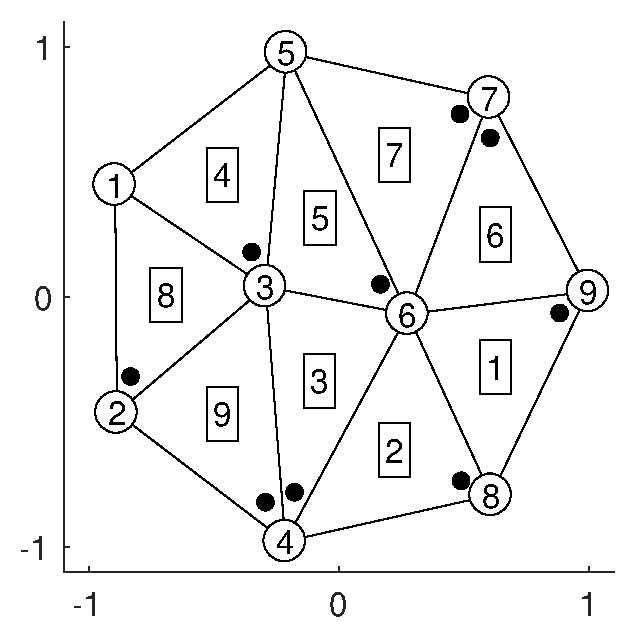
\includegraphics[width=0.4\textwidth]{fe_mesh_p1}
  }
  \caption{Triangulation.}
  \label{fig:fe_mesh_p1}
\end{figure}

While mathematically a triangulation is simply a collection of non-overlapping elements, we need a convenient means to represent the triangulation on a computer.  One approach is to store tables of \emph{node coordinates} and \emph{element-node connectivities}.  Tables~\ref{tb:fe_mesh_p1_coord} and \ref{tb:fe_mesh_p1_tri} are respectively the coordinate and connectivity tables associated with the triangulation shown in Figure~\ref{fig:fe_mesh_p1}. The connectivity table indicates that, for instance, element 5 is delineated by the nodes 6, 5, and 3; the coordinate table then indicates that the coordinates of these three nodes are $(0.28,-0.07)$, $(-0.21,0.98)$, and $(-0.29,0.04)$, respectively.  Note that, in Figure~\ref{fig:fe_mesh_p1}, for each triangle, we indicate the first of the three nodes that delineate the triangle by a dot ($\bullet$); with this convention we have identical information presented in Figure~\ref{fig:fe_mesh_p1} in a visual form and Tables~\ref{tb:fe_mesh_p1_coord} and \ref{tb:fe_mesh_p1_tri} in an array form.

\begin{table}
  \centering
  \caption{Node coordinate and connectivity table for mesh shown in Figure~\ref{fig:fe_mesh_p1}.  \label{tb:fe_mesh_p1}}
    \subfigure[coordinates]{
      \label{tb:fe_mesh_p1_coord}
    \begin{tabular}{c|cc}
      node & $x_1$ & $x_2$ \\
      \hline
      $1$ & $-0.89$ & $\hphantom{-}0.45$ \\ 
      $2$ & $-0.89$ & $-0.46$ \\ 
      $3$ & $-0.29$ & $\hphantom{-}0.04$ \\ 
      $4$ & $-0.21$ & $-0.98$ \\ 
      $5$ & $-0.21$ & $\hphantom{-}0.98$ \\ 
      $6$ & $\hphantom{-}0.28$ & $-0.07$ \\ 
      $7$ & $\hphantom{-}0.60$ & $\hphantom{-}0.80$ \\ 
      $8$ & $\hphantom{-}0.61$ & $-0.79$ \\ 
      $9$ & $\hphantom{-}1.00$ & $\hphantom{-}0.02$ \\ 
    \end{tabular}
  }
    \subfigure[connectivity]{
          \label{tb:fe_mesh_p1_tri}
    \begin{tabular}{c|ccc}
      element & node 1 & node 2 & node 3 \\
      \hline
      $1$ & $9$ & $6$ & $8$ \\ 
      $2$ & $8$ & $6$ & $4$ \\ 
      $3$ & $4$ & $6$ & $3$ \\ 
      $4$ & $3$ & $5$ & $1$ \\ 
      $5$ & $6$ & $5$ & $3$ \\ 
      $6$ & $7$ & $6$ & $9$ \\ 
      $7$ & $7$ & $5$ & $6$ \\ 
      $8$ & $2$ & $3$ & $1$ \\ 
      $9$ & $4$ & $3$ & $2$ \\ 
    \end{tabular}
    }
\end{table}

The task of generating a triangulation for a given domain is called \emph{mesh generation} and a program that carries out the task is called a \emph{mesh generator} or \emph{mesher}.  Mesh generation is a non-trivial task.  In fact, the development of algorithms that can robustly and automatically generate high-quality triangulation for complex geometries in three dimensions is an area of ongoing research.  Nevertheless, because mesh generation is essential for any finite element discretization, there are many commercial and open-source meshers.  Here we name a few user-friendly, open-source meshers:
\begin{itemize}
\item \texttt{triangle}. A robust two-dimensional mesher written in C that generates meshes with a guaranteed quality certificate in terms of the minimal angle.
\item \texttt{tetgen}. A popular three-dimensional mesher written in C.
\item \texttt{distmesh}.  A user-friendly mesher written in \textsc{Matlab} for implicit domain geometries represented by level sets. 
\end{itemize}
The mesh shown in Figure~\ref{fig:fe_mesh_p1} was in fact generated by \texttt{distmesh}.  We will extensively use \texttt{distmesh} to generate meshes in this course as it is implemented in \textsc{Matlab} and is easy to use.


\section{Approximation spaces}
We now introduce \emph{approximation spaces} for $\calV$.  An approximation space is a finite-dimensional subspace space of $\calV$ with which we can approximate functions in $\calV$.  For concreteness, we consider a piecewise-polynomial approximation space associated with the triangulation $\calT_h$. For simplicity, we first consider the case $\calV \equiv H^1(\Omega)$:
\begin{equation*}
  \calV_h \equiv \{ v \in \calV \equiv H^1(\Omega) \ | \ v|_K \in \PP^p(K), \ K \in \calT_h \},
  \label{eq:fe_Vh}
\end{equation*}
where $\PP^p(K)$ is the space of polynomials of degree at most $p$ over $K$.
We note the two requirements: $v \in \calV_h$ must belong to $\calV \equiv H^1(\Omega)$; 
%We note the two requirements: $v \in \calV_h$ must belong to $\calV \subset H^1(\Omega)$ and in particular satisfy the essential boundary conditions;
$v$ restricted to any element $K \in \calT_h$, $v|_K$, must be a polynomial of degree $p$. Figure~\ref{fig:fe_fun_p1} shows an example of a function in a linear ($\PP^1$) finite element space,
\begin{equation}
  \calV_h \equiv \{ v \in \calV \equiv H^1(\Omega) \ | \ v|_K \in \PP^1(K), \ K \in \calT_h \},
  \label{eq:fe_lin_Vh}
\end{equation}
associated with the mesh shown in Figure~\ref{fig:fe_mesh_p1}.

\begin{figure}
  \centering
  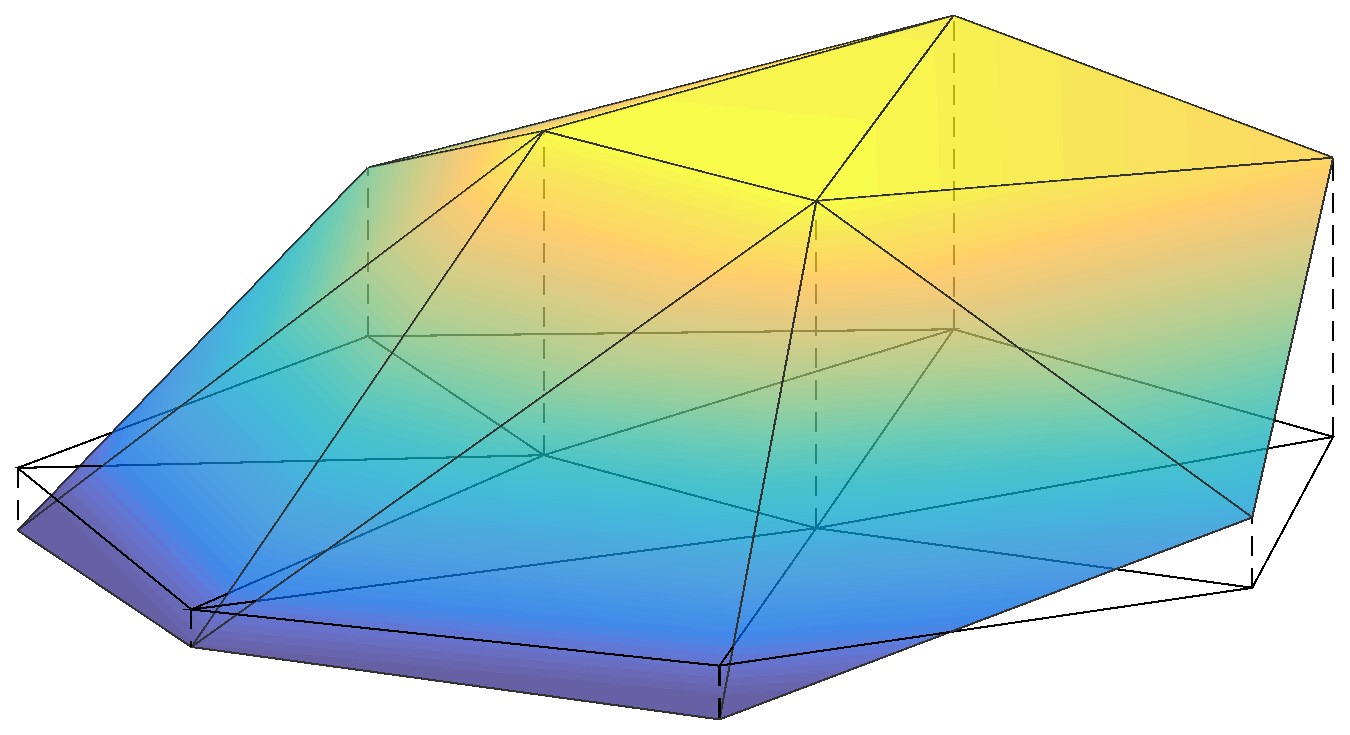
\includegraphics[width=0.45\textwidth]{fe_fun_p1}
  \caption{A function in a linear finite element space.}
  \label{fig:fe_fun_p1}
\end{figure}

We note that the condition $\calV_h \subset \calV \subset H^1(\Omega)$ means that the weak derivative of functions must be square integrable (in the Lebesgue sense); for piecewise polynomials, the condition is satisfied if and only if the function is continuous.  To see this, we observe the following.  If a function is continuous and piecewise polynomial, the weak first derivative is potentially discontinuous but is piecewise polynomial and hence is square integrable; the function hence is in $H^1(\Omega)$.  If a function is not continuous across element interfaces, then the weak first derivative generates delta distributions at the interfaces and hence is not in $L^2(\Omega)$; recall for instance a concrete example for a Heaviside-like function in Section~\ref{sec:posnd_sobolev}. Hence, for a piecewise polynomial function, the continuity is the necessary and sufficient condition for the function to be in $H^1(\Omega)$. 

We now need a convenient means to describe functions in $\calV_h$ given by~\eqref{eq:fe_lin_Vh}, such as the one shown in Figure~\ref{fig:fe_fun_p1}.  Specifically, we need to pick \emph{global degrees of freedom} with which we can uniquely describe any function in $\calV_h$. To this end, we introduce a \emph{basis} for the linear space $\calV_h$.  We recall that a set of functions $\{ \phi_i \}_{i=1}^n$ is a basis for $\calV_h$ if the set (i) spans $\calV_h$ and (ii) is linearly independent. The first requirement implies that any $w \in \calV_h$ can be expressed as a linear combination of $\{ \phi_i \}_{i=1}^n$.  The second requirement implies that the coefficients associated with the representation of $w \in \calV_h$ in terms of $\{ \phi_i \}_{i=1}^n$ is unique.  In other words, if $\{ \phi_i \}_{i=1}^n$ is a basis for $\calV_h$, then for any $w \in \calV_h$ there exists a unique $\hat w \in \RR^n$ such that
\begin{equation*}
  w = \sum_{j=1}^n \hat w_j \phi_j
\end{equation*}
for $n = \text{dim}(\calV_h)$.

While the choice of a basis is not unique, one convenient choice is a \emph{Lagrange basis} or \emph{nodal basis}.  Nodal basis comprises functions that take on the value of 1 at the associated node and 0 at all other nodes:
\begin{equation}
  \phi_j(x_i) = \delta_{ij},
  \label{eq:fe_lagrange_basis_prop}
\end{equation}
where $\delta_{ij}$ is the Kronecker delta so that $\delta_{ij} = 1$ if $i = j$ and $\delta_{ij} = 0$ if $i \neq j$. Figure~\ref{fig:fe_shape_global_p1} shows an example of a basis function, $\phi_3$, for the linear finite element space~\eqref{eq:fe_lin_Vh} associated with the mesh shown in Figure~\ref{fig:fe_mesh_p1}.  For $\calV_h$ defined by~\eqref{eq:fe_lin_Vh}, there are nine nodal basis functions, one associated with each node.  We also observe that the set of the nine functions indeed forms a basis: the set is linearly independent and spans the space. The set is linearly independent because $\sum_{j=1}^n \hat w_j \phi_j = 0$ implies $\sum_{j=1}^n \hat w_j \phi_j(x_i) = 0$, $\forall i =1,\dots,n$, which in turn implies $\hat w_j = 0$, $j = 1,\dots,n$.  The set spans the space because the piecewise linear polynomial space is nine dimensional and the linearly independent set contains nine functions.

\begin{figure}
  \centering
  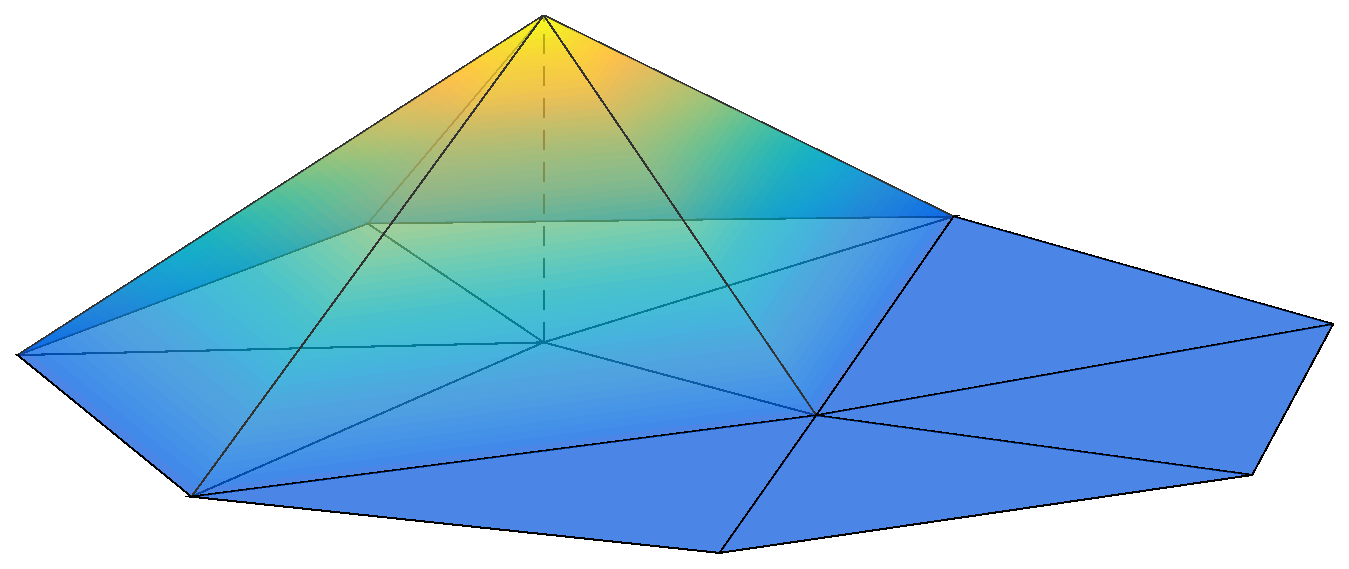
\includegraphics[width=0.48\textwidth]{shape_global_p1}
  \caption{Nodal basis $\phi_3$ for the linear finite element space $\calV_h$ defined by \eqref{eq:fe_lin_Vh}.}
  \label{fig:fe_shape_global_p1}
\end{figure}

While the choice of a basis not unique, the nodal basis provides a convenient interpretation in the physical space.  Specifically, for $w \in \calV_h$, we have a (unique) representation
\begin{equation}
  w = \sum_{j=1}^n \hat w_j \phi_j = \sum_{j=1}^n w(x_j) \phi_j.
  \label{eq:fe_rep}
\end{equation}
We note that the coefficient $\hat w_j$ must be equal to $w(x_j)$, because $w(x_i) = \sum_{j=1}^n \hat w_j \phi_j(x_i) = \sum_{j=1}^n \hat w_j \delta_{ij} = \hat w_i$, $i = 1,\dots,n$; here, the second equality follows from the Lagrange interpolation property~\eqref{eq:fe_lagrange_basis_prop}.  In words, $\hat w_j = w(x_j)$, the value of the function $w \in \calV_h$ evaluated at the associated node $x_j$. This interpretation of nodal basis allows us to readily confirm that the nodal basis is indeed a basis: for any $w \in \calV_h$, there exists a unique $\hat w \in \RR^n$ such that $w = \sum_{j=1}^n \hat w_j \phi_j$.  We can clearly express any function $w \in \calV_h$ in the form~\eqref{eq:fe_rep}; moreover the representation is unique. 

\section{Approximation spaces: essential boundary conditions}
We recall from Lecture~\ref{ch:var_form} that Dirichlet boundary conditions are treated as essential boundary conditions in the weak formulation of second-order elliptic PDEs.  For instance, given a mixed Poisson problem on $\Omega \subset \RR^d$ with a Dirichlet boundary $\Gamma_D \subset \partial \Omega$, the appropriate function space is
\begin{equation*}
  \calV \equiv \{ v \in H^1(\Omega) \ | \ v|_{\Gamma_D} = 0 \}.
\end{equation*}
The functions in the associated approximation space $\calV_h$ must also vanish on $\Gamma_D$ so that $\calV_h \subset \calV$.  With nodal basis, we can readily enforce this condition by eliminating the basis functions associated with the nodes on the (closure of the) Dirichlet boundary $\overline \Gamma_D$ from the approximation space. The dimension of the resulting approximation space for $\calV \subset H^1(\Omega)$ is
\begin{equation*}
  n = \text{dim}(\calV_h) = (\text{dimension of approximation space for $H^1(\Omega)$}) - (\text{number of Dirichlet nodes}).
\end{equation*}
Then, as before, we can express any function in $w \in \calV_h$ as
\begin{equation*}
  w = \sum_{j=1}^n \hat w_j \phi_j,
\end{equation*}
where the basis $\{ \phi_j \}_{j=1}^n$ consists of nodal basis associated with nodes not on the (closure of the) Dirichlet boundary.

We now consider the construction of an approximation space for an affine space of the form
\begin{equation*}
  \calV^E \equiv u^E + \calV,
\end{equation*}
where $u^E$ is an arbitrary member in $H^1(\Omega)$ that satisfies the boundary condition $u^E|_{\Gamma_D} = u^B$.  In general, 


\begin{equation*}
  w = u^E_h + \sum_{j=1}^n \hat w_j \phi_j
\end{equation*}
  


\section{Galerkin method}
We first recall the weak formulation for the exact problem: find $u \in \calV$ such that
\begin{equation}
  a(u,v) = \ell(v) \quad \forall v \in \calV,
  \label{eq:fe_form_true}
\end{equation}
where $a: \calV \times \calV \to \RR$ is a coercive, continuous bilinear form and $\ell: \calV \to \RR$ is a continuous linear form. We now seek an approximation to~\eqref{eq:fe_form_true} in a (finite-dimensional) subspace $\calV_h \subset \calV$: find $u_h \in \calV_h$ such that
\begin{equation}
  a(u_h,v) = \ell(v) \quad \forall v \in \calV_h.
  \label{eq:fe_form_gal_0}
\end{equation}
In words, we obtain the finite-element problem by simply replacing test and trials spaces by $\calV_h \subset \calV$.  Because the trial and test approximation spaces are the same, the method is referred to as the \emph{Galerkin method}.  (If the test and trial approximation spaces are different, the method is referred to as the \emph{Petrov-Galerkin method}.) We also note that the finite element problem~\eqref{eq:fe_form_gal_0} depends on the space $\calV_h$ but is independent of the particular basis $\{ \phi_i \}_{i=1}^n$ for $\calV_h$.  We will prove in Section~\ref{sec:fe_form_gal_wellposed} that~\eqref{eq:fe_form_gal_0} has a unique solution.

We now wish to recast the finite element problem~\eqref{eq:fe_form_gal_0} in linear algebraic from that is amenable to computer implementation.  To this end, we represent the solution and test functions in terms of their basis coefficients, $u_h = \sum_{j=1}^n \hat u_{h,j} \phi_j$ and $v = \sum_{i=1}^n \hat v \phi_i$ to yield the following equivalent problem for the coefficients: find $\hat u_h \in \RR^n$ such that
\begin{equation*}
  a(\sum_{j=1}^n \hat u_{h,j} \phi_j, \sum_{i=1}^n \hat v_i \phi_i)
  = \ell(\sum_{i=1}^n \hat v_i \phi_i) \quad \forall \hat v \in \RR^n.
\end{equation*}
We then invoke the bilinearity of $a(\cdot,\cdot)$ and the linearity of $\ell(\cdot)$ to obtain
\begin{equation*}
  \sum_{i,j = 1}^n \hat v_i a(\phi_j,\phi_i) \hat u_{h,j} = \sum_{i=1}^n \hat v_i \ell(\phi_i).
\end{equation*}
The problem can be more compactly expressed using the matrix-vector notation: find $\hat u_h \in \RR^n$ such that
\begin{equation}
  \hat v^T \hat A_h \hat u_h = \hat v^T \hat f_h \quad \forall \hat v \in \RR^n,
  \label{eq:fe_form_gal_3}
\end{equation}
where the \emph{stiffness matrix} $\hat A_h \in \RR^{n \times n}$ is given by
\begin{equation*}
  \hat A_{h,ij} \equiv a(\phi_j, \phi_i), \quad i,j = 1,\dots,n,
\end{equation*}
and the \emph{load vector} $\hat f_h \in \RR^n$ is given by
\begin{equation*}
  \hat f_{h,i} \equiv \ell(\phi_i), \quad i = 1,\dots,n.
\end{equation*}
In order for~\eqref{eq:fe_form_gal_3}, each row of $A_h \hat u_h - f_h$ must be equal to zero; otherwise, we can find $\hat v \in \RR^n$ that is finite only on that non-zero and hence~\eqref{eq:fe_form_gal_3} would not hold.  We hence conclude that the statement \eqref{eq:fe_form_gal_3} is equivalent to finding $\hat u_h \in \RR^n$ that satisfies 
\begin{equation}
  \hat A_h \hat u_h = \hat f_h  \quad \text{(in $\RR^n$)}.
  \label{eq:fe_form_gal_4}
\end{equation}
We will prove in Section~\ref{sec:fe_form_gal_wellposed} that~\eqref{eq:fe_form_gal_4} has a unique solution.

\section{Well-posedness of the Galerkin finite element formulation}
\label{sec:fe_form_gal_wellposed}
We now wish to show that~\eqref{eq:fe_form_gal_0} has a unique solution and is well-posed.
\begin{proposition}
  \label{prop:fe_form_gal_wellposed}
    Given an approximation space $\calV_h \subset \calV$, a continuous, coercive bilinear form $a: \calV \times \calV \to \RR$, and a continuous linear functional $\ell \in \calV'$, there exists a unique $u_h \in \calV_h$ such that
  \begin{equation*}
    a(u_h,v) = \ell(v) \quad \forall v \in \calV_h.
  \end{equation*}
  \begin{proof}
We will appeal to the Lax-Milgram theorem, Theorem~\ref{thm:lax_milgram}; to do so, we need to demonstrate that (i) the bilinear form $a(\cdot,\cdot)$ is coercive in $\calV_h$, (ii) the bilinear form is continuous $a(\cdot,\cdot)$ is continuous in $\calV_h$, and (iii) the linear form $\ell(\cdot)$ is continuous in $\calV_h$.  The coercivity of $a(\cdot,\cdot)$ in $\calV_h$ follows form
\begin{equation*}
  \alpha_h \equiv \inf_{v \in \calV_h} \frac{a(v,v)}{\| v \|_\calV} \geq
  \inf_{v \in \calV} \frac{a(v,v)}{\| v \|_\calV} \equiv \alpha > 0,
\end{equation*}
where the inequality follows from $\calV_h \subset \calV$.  The coercivity constant associated with $\calV_h$, $\alpha_h$, is bounded from the below by the coercivity constant associated with $\calV$, $\alpha$, which itself is bounded from the below by $0$. The continuity of $a(\cdot,\cdot)$ in $\calV_h$ follows from
\begin{equation*}
  \gamma_h \equiv \sup_{v \in \calV_h} \frac{a(v,v)}{\| v \|_\calV} \leq
  \sup_{v \in \calV} \frac{a(v,v)}{\| v \|_\calV} \equiv \gamma < \infty,
\end{equation*}
where the inequality again follows from $\calV_h \subset \calV$.  The continuity constant associated with $\calV_h$, $\gamma_h$, is bounded from the above by the continuity constant associated with $\calV$, $\gamma$, which itself is finite.  Similarly, the continuity of $\ell(\cdot)$ in $\calV_h$ follows from
\begin{equation*}
  \| \ell \|_{(\calV_h)'} \equiv \sup_{v \in \calV_h} \frac{\ell(v)}{\| v \|_\calV} \leq \sup_{v \in \calV} \frac{\ell(v)}{\| v \|_\calV} \equiv \| \ell \|_{\calV'} < \infty,
\end{equation*}
where the inequality again follows from $\calV_h \subset \calV$.  Because the bilinear from is coercive and continuous in $\calV_h$ and the linear from is continuous in $\calV_h$, we conclude by the Lax-Milgram theorem that the solution exists and is unique.
  \end{proof}
\end{proposition}
The proposition shows the existence of a unique solution to the finite element problem~\eqref{eq:fe_form_gal_0} without appealing to any specific basis for $\calV_h$; the finite element solution $u_h \in \calV_h$ (perhaps not too surprisingly) depends only on the space $\calV_h$ and is independent of the specific basis $\{ \phi_i \}_{i=1}^n$ used to represent the solution.

We can also show that the linear algebraic problem~\ref{eq:fe_form_gal_4} associated with the basis coefficients, $\hat A_h \hat u_h = \hat f_h$, is well-posed.  One way to prove the existence of unique coefficients is to appeal to (i) the existence and uniqueness of $u_h \in \calV_h$ by Proposition~\eqref{prop:fe_form_gal_wellposed} and (ii) the existence and uniqueness of the associated basis-specific representation $u_h = \sum_{i=1}^n \hat u_{h,i} \phi_i$ since $\{\phi_i\}_{i=1}^n$ is a basis for $\calV_h$. Alternatively, we can directly show that the matrix $\hat A_h \in \RR^{n \times n}$ is symmetric positive definite and hence is non-singular. 
\begin{proposition}
  If the bilinear form $a: \calV \times \calV \to \RR$ is symmetric and coercive, then the stiffness matrix $\hat A_h \in \RR^{n \times n}$ is symmetric positive definite (SPD).
  \begin{proof}
    The symmetry of $\hat A_h$ follows directly from the symmetry of the bilinear form:
  \begin{equation*}
    \hat A_{h,ij} = a(\phi_j,\phi_i) = a(\phi_i,\phi_j) = \hat A_{h,ji}.
  \end{equation*}
  To prove positive definiteness, we first observe that $\forall \hat v \in \RR^n$, 
\begin{equation*}
  \hat v^T \hat A_{h} \hat v
  =
  \sum_{i,j = 1}^n \hat v_i a(\phi_j, \phi_i) \hat v_j 
  = a(\sum_{j=1}^n \hat v_j \phi_j, \sum_{i=1}^n \hat v_i \phi_i)
  \geq \alpha \| \sum_{i=1}^n \hat v_i \phi_i \|^2_{\calV} \geq 0,
\end{equation*}
where the first inequality follows from the coercivity of $a(\cdot,\cdot)$ and the last equality follows from the positive definiteness of the norm $\| \cdot \|_{\calV}$. Moreover, because $\| \cdot \|_{\calV}$ is a norm, $\| \sum_{i=1}^n \hat v_i \phi_i \|_\calV = 0$ if and only if $\sum_{i=1}^n \hat v_i \phi_i = 0$.  In addition, because $\{\phi_i\}_{i=1}^n$ is a basis and in particular linearly independent, $\sum_{i=1}^n \hat v_i \phi_i = 0$ if and only if $\hat v_i = 0$, $\forall i = 1,\dots,n$. It follows that
\begin{equation*}
  \hat v^T \hat A_h \hat v = 0 \quad \text{if and only if} \quad \hat v = 0.
\end{equation*}
Hence, the matrix $\hat A_h \in \RR^{n \times n}$ is SPD.
  \end{proof}
\end{proposition}


\section{Minimization formulation: Rayleigh-Ritz formulation}
We now seek the finite element approximation to the problem using the minimization formulation. To this end, we recall that the energy functional is given by 
\begin{align*}
  J(w) =  J(\sum_{j=1}^n \hat w_j \phi_j)
  = \frac{1}{2} a (\sum_{j=1}^n \hat w_j \phi_j, \sum_{i=1}^n \hat w_i \phi_i) - \ell(\sum_{i=1}^n \hat w_i \phi_i)
  = \frac{1}{2} \sum_{i,j=1}^n \hat w_i a(\phi_j,\phi_i) \hat w_j - \sum_{i=1}^n \hat w_i \ell(\phi_i)
\end{align*}

\begin{equation*}
  (\hat A_h)_{ij} \equiv a(\phi_j,\phi_i)
  \quad \text{and} \quad
  (\hat f_h)_i \equiv \ell(\phi_i)
\end{equation*}

\begin{equation*}
  \hat J(\hat w) = J(\sum_{j=1}^n \hat w_j \phi_j)
  = \frac{1}{2} \hat w^T \hat A_h \hat w - \hat w^T \hat f_h
\end{equation*}

\begin{equation*}
  \hat u_h = \argmin_{\hat w \in \RR^n} \hat J(\hat w)
\end{equation*}

\begin{equation*}
  \nabla \hat J(\hat u_h) = \hat A_h \hat u_h - \hat f_h = 0
\end{equation*}

\section{Generalization}
In this lecture, we considered an approximation space based on piecewise polynomials and constructed the associated Galerkin (and Rayleigh-Ritz) approximation. However, the Galerkin (and Rayleigh-Ritz) procedure are in fact general projection procedure that works with any approximation spaces. For instance, the \emph{spectral method} is an approximation 
\begin{equation*}
  \calV_p \equiv \{ v \in \calV \ | \ v \in \PP^p(\Omega) \}.
\end{equation*}

\chapter{Finite element method: implementation}
\section{Linear Lagrange finite element}
\label{sec:fe_lin_tri}
%% We now consider the construction of a piecewise linear polynomial space associated with the triangulation $\calT_h$. We recall that our variational (or weak) formulation requires that the finite element space is a subset of the function space for the exact PDE, which, for second-order elliptic equations, is some $\calV$ which is a subset of $H^1(\Omega)$. Since our finite element space $\calV_h$ is piecewise polynomial, the continuity across element boundaries is the necessary and sufficient condition for $\calV_h \subset \calV$.  Hence, our goal is to devise a systematic procedure to represent any functions in
%% \begin{equation}
%%   \calV_h \equiv \{ v \in C^0(\overline \Omega) \ | \ v|_K \in \PP^1(K), \ K \in \calT_h \},
%%   \label{eq:fe_lin_Vh}
%% \end{equation}
%% where $C^0(\overline \Omega)$ is the space of continuous functions over $\overline \Omega$.  Figure~\ref{fig:fe_fun_p1} shows an example of a continuous, piecewise-linear function in $\calV_h$ associated with $\calT_h$ shown in Figure~\ref{fig:fe_mesh_p1}.
%% \begin{figure}
%%   \centering
%%   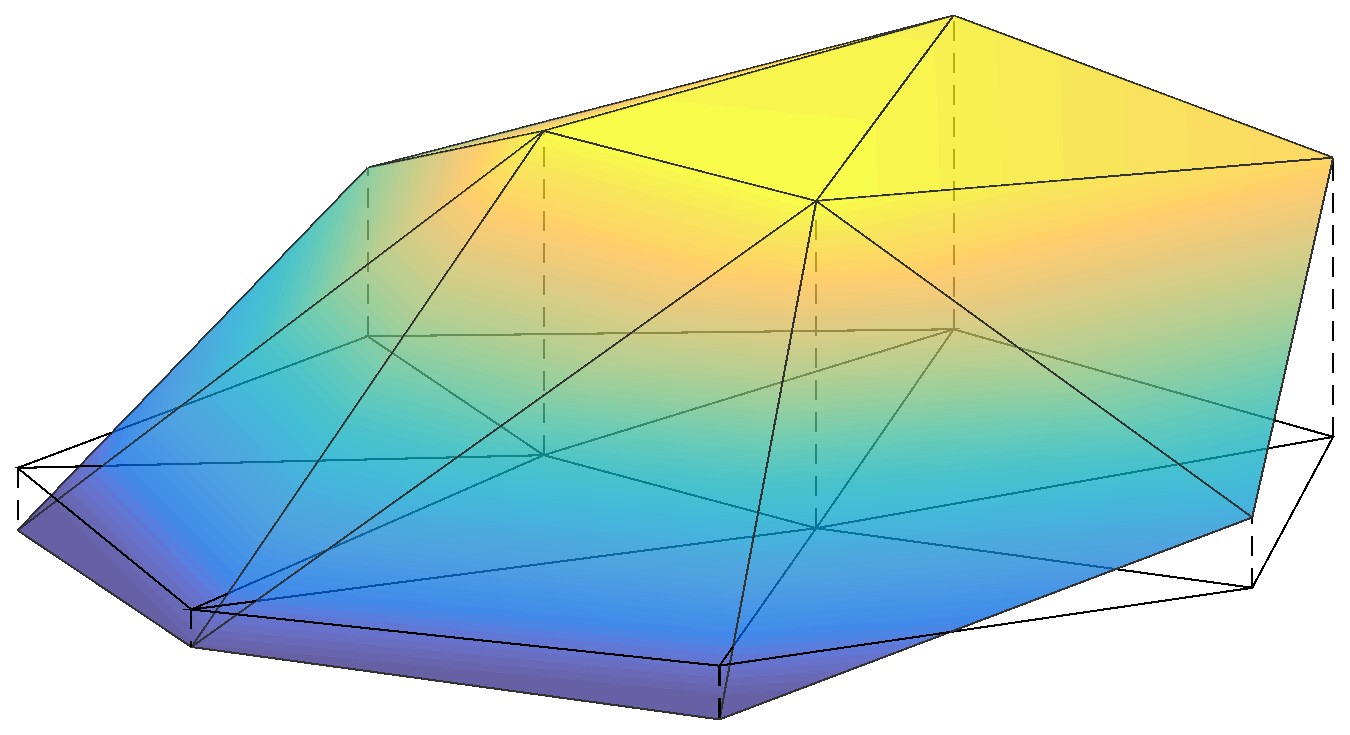
\includegraphics[width=0.45\textwidth]{fe_fun_p1}
%%   \caption{A function in a linear finite element space.}
%%   \label{fig:fe_fun_p1}
%% \end{figure}


As we have seen in Lecture~\ref{ch:pos1d}, the computation of a finite element solution requires a few common tasks on the functions in $\calV_h$, such as the evaluation of the function values, the valuation of the gradient values, and the integration of the functions.  Our approach to construct the piecewise polynomial space is to first define a polynomial space on a \emph{reference element} (or a \emph{canonical element}) and then to map the polynomial functions to the actual elements that comprise the triangulation.  As such, we first introduce the \emph{reference triangle} $\tilde K$.  While the definition of a reference triangle is not universal, our reference triangle is shown in Figure~\ref{fig:fe_ref_tri}.  The triangle is a right triangle delineated by three vertices
\begin{equation*}
  v^1 \equiv (0,0), \quad v^2 \equiv (1,0), \quad \text{and} \quad v^3 \equiv (0,1).
\end{equation*}
The vertices are ordered in the counter-clockwise manner. We also denote the three edges of the triangles by
\begin{equation*}
  e^1 \equiv (v^2,v^3), \quad e^2 \equiv (v^3,v^1), \quad \text{and} \quad e^3 \equiv (v^1,v^2).
\end{equation*}
We choose the convention that the edge number is the same as the vertex number of the vertex on the other side of the triangle. Each edge is oriented such that the collection of the three edges defines the triangle in the counter-clock orientation.  

\begin{figure}
  \centering
  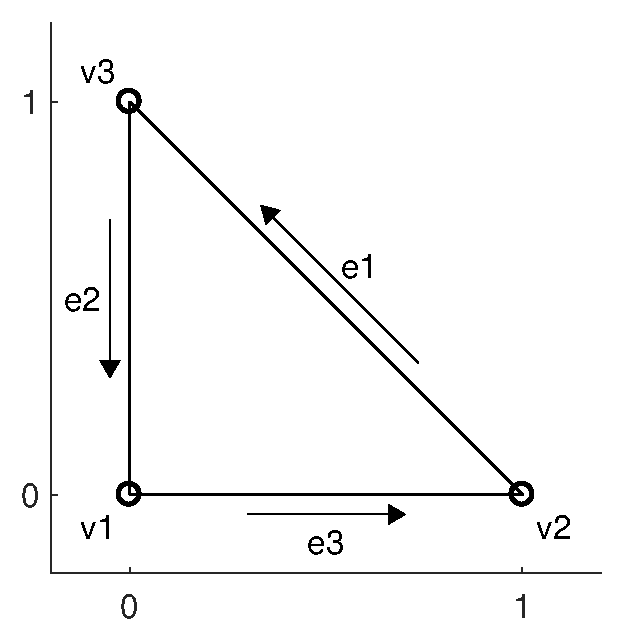
\includegraphics[width=0.3\textwidth]{ref_tri}
  \caption{Reference triangle.}
  \label{fig:fe_ref_tri}
\end{figure}

Having introduced the reference triangle, we now introduce arguably the simplest finite element in two dimensions: linear Lagrange element on the reference triangle. A linear function in $\PP^1(\tilde K)$ takes on the form $a_1 + a_2 \tilde x_1 + a_3 \tilde x_2$ and has three degrees of freedom; we hence need to identify a linear independent set of three linear functions.  In our case, we wish to identify a set of three linear \emph{Lagrange basis functions} for the space.  To this end, we choose for our Lagrange interpolation nodes the three vertices of the triangle
\begin{equation*}
  \tilde x^{(1)} = (0,0), \quad \tilde x^{(2)} = (1,0), \quad \text{and} \quad \tilde x^{(3)} = (0,1),
\end{equation*}
as shown in Figure~\ref{fig:fe_ref_tri_p1}. Our goal is to find the Lagrange basis functions
\begin{equation*}
  \{ \tilde \phi_1, \tilde \phi_2, \tilde \phi_3 \}
\end{equation*}
that lie in the $\PP^1(\tilde K)$ space and satisfy the interpolation condition
\begin{equation}
  \tilde \phi_i(\tilde x^{(j)}) = \delta_{ij} \quad i,j = 1,\dots,3.
% \equiv
% \begin{cases}
%   1, \quad i = j \\
%%   0, \quad i \neq j
% \end{cases};
   \label{eq:fe_interp_tri}
\end{equation}
Here, $\delta_{ij}$ denotes the \emph{Kronecker delta} such that $\delta_{ij} = 1$ for $i = j$ and $\delta_{ij} = 0$ for $i \neq j$.

\begin{figure}
  \centering
  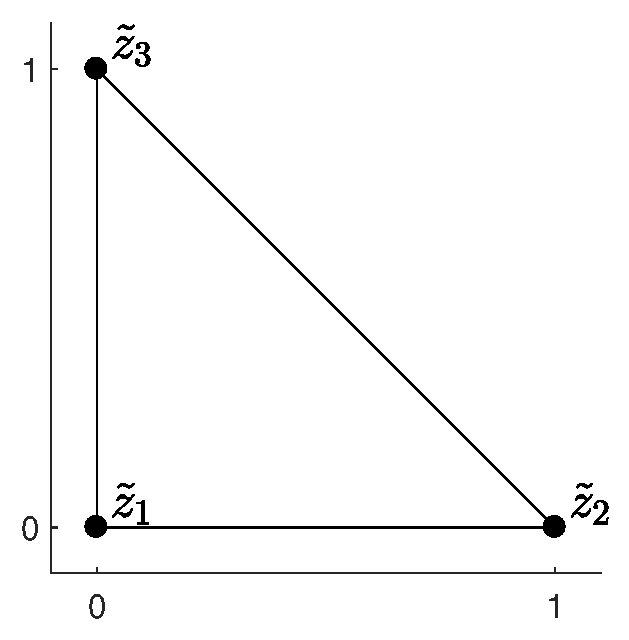
\includegraphics[width=0.3\textwidth]{ref_tri_p1}
  \caption{Linear Lagrange finite element on the reference triangle.}
  \label{fig:fe_ref_tri_p1}
\end{figure}


    While we may identify the Lagrange basis functions for the linear space by inspection, we here follow a more systematic procedure that apply to more complex domains and higher-order polynomials.  To this end, we first note that any linear function can be expressed as a linear combination of a monomial basis
\begin{equation*}
  \{ 1, \tilde x_1, \tilde x_2\}.
\end{equation*}
Since linear Lagrange basis functions are also linear functions, we can express the basis functions in terms of the monomial basis:
\begin{equation}
  \tilde \phi_j(\tilde x) = a^{(j)}_1 + a^{(j)}_2 \tilde x_1 + a_3^{(j)} \tilde x_2 \quad j = 1, 2, 3.
  \label{eq:fe_lin_tri_rep}
\end{equation}
We now apply the interpolation condition~\eqref{eq:fe_interp_tri} to find the coefficients.  For instance, $\tilde \phi_1$ must satisfy
\begin{equation*}
  \bmat{ccc}
  1 & \tilde x_1^{(1)} & \tilde x_2^{(1)} \\
  1 & \tilde x_1^{(2)} & \tilde x_2^{(2)} \\
  1 & \tilde x_1^{(3)} & \tilde x_2^{(3)} \\
  \emat
  \bmat{ccc}
  a_1^{(1)} \\ a_2^{(1)} \\ a_3^{(1)}
  \emat
  =
  \bmat{ccc}
  1 \\ 0 \\ 0.
  \emat
\end{equation*}
We can also pose a single matrix equation for the monomial coefficients of all three shape functions: 
\begin{equation*}
  \underbrace{ \bmat{ccc}
      1 & \tilde x_1^{(1)} & \tilde x_2^{(1)} \\
  1 & \tilde x_1^{(2)} & \tilde x_2^{(2)} \\
  1 & \tilde x_1^{(3)} & \tilde x_2^{(3)} \\
  \emat }_{\equiv V}
  \underbrace{ 
  \bmat{ccc}
  a_1^{(1)} & a_1^{(2)} & a_1^{(3)} \\
  a_2^{(1)} & a_2^{(2)} & a_2^{(3)} \\
  a_3^{(1)} & a_3^{(2)} & a_3^{(3)} \\
  \emat
  }_{\equiv A}
  =
  \bmat{ccc}
  1 & 0 & 0 \\
  0 & 1 & 0 \\
  0 & 0 & 1
  \emat.
\end{equation*}
We note that the matrix $V$ in the left hand side is the \emph{Vandermonde matrix} associated with our monomial basis evaluated at the Lagrange interpolation points $\{\tilde x^{(1)},\tilde x^{(2)}, \tilde x^{(3)}\}$.  The matrix $V$ is non-singular as long as the interpolation points are not collinear, which is equivalent to the condition that the triangle have a finite area; the condition is obviously satisfied for our reference triangle $\tilde K$.  For completeness, we provide the explicit expression for the coefficient $A$
\begin{equation*}
  A = \bmat{ccc}
  1 & 0 & 0\\
  -1 & 1 & 0 \\
  -1 & 0 & 1
  \emat,
\end{equation*}
the explicit expressions for the basis functions
\begin{align}
  \tilde \phi_1(\tilde x) &= 1 - \tilde x_1 - \tilde x_2 \notag \\
  \tilde \phi_2(\tilde x) &= \tilde x_1 \label{eq:fe_lin_tri_expl} \\
  \tilde \phi_3(\tilde x) &= \tilde x_2, \notag
\end{align}
and in Figure~\ref{fig:fe_shape_tri_p1} visual representation of the basis functions.

\begin{figure}
  \centering
  \subfigure[$\tilde \phi_1$]{
    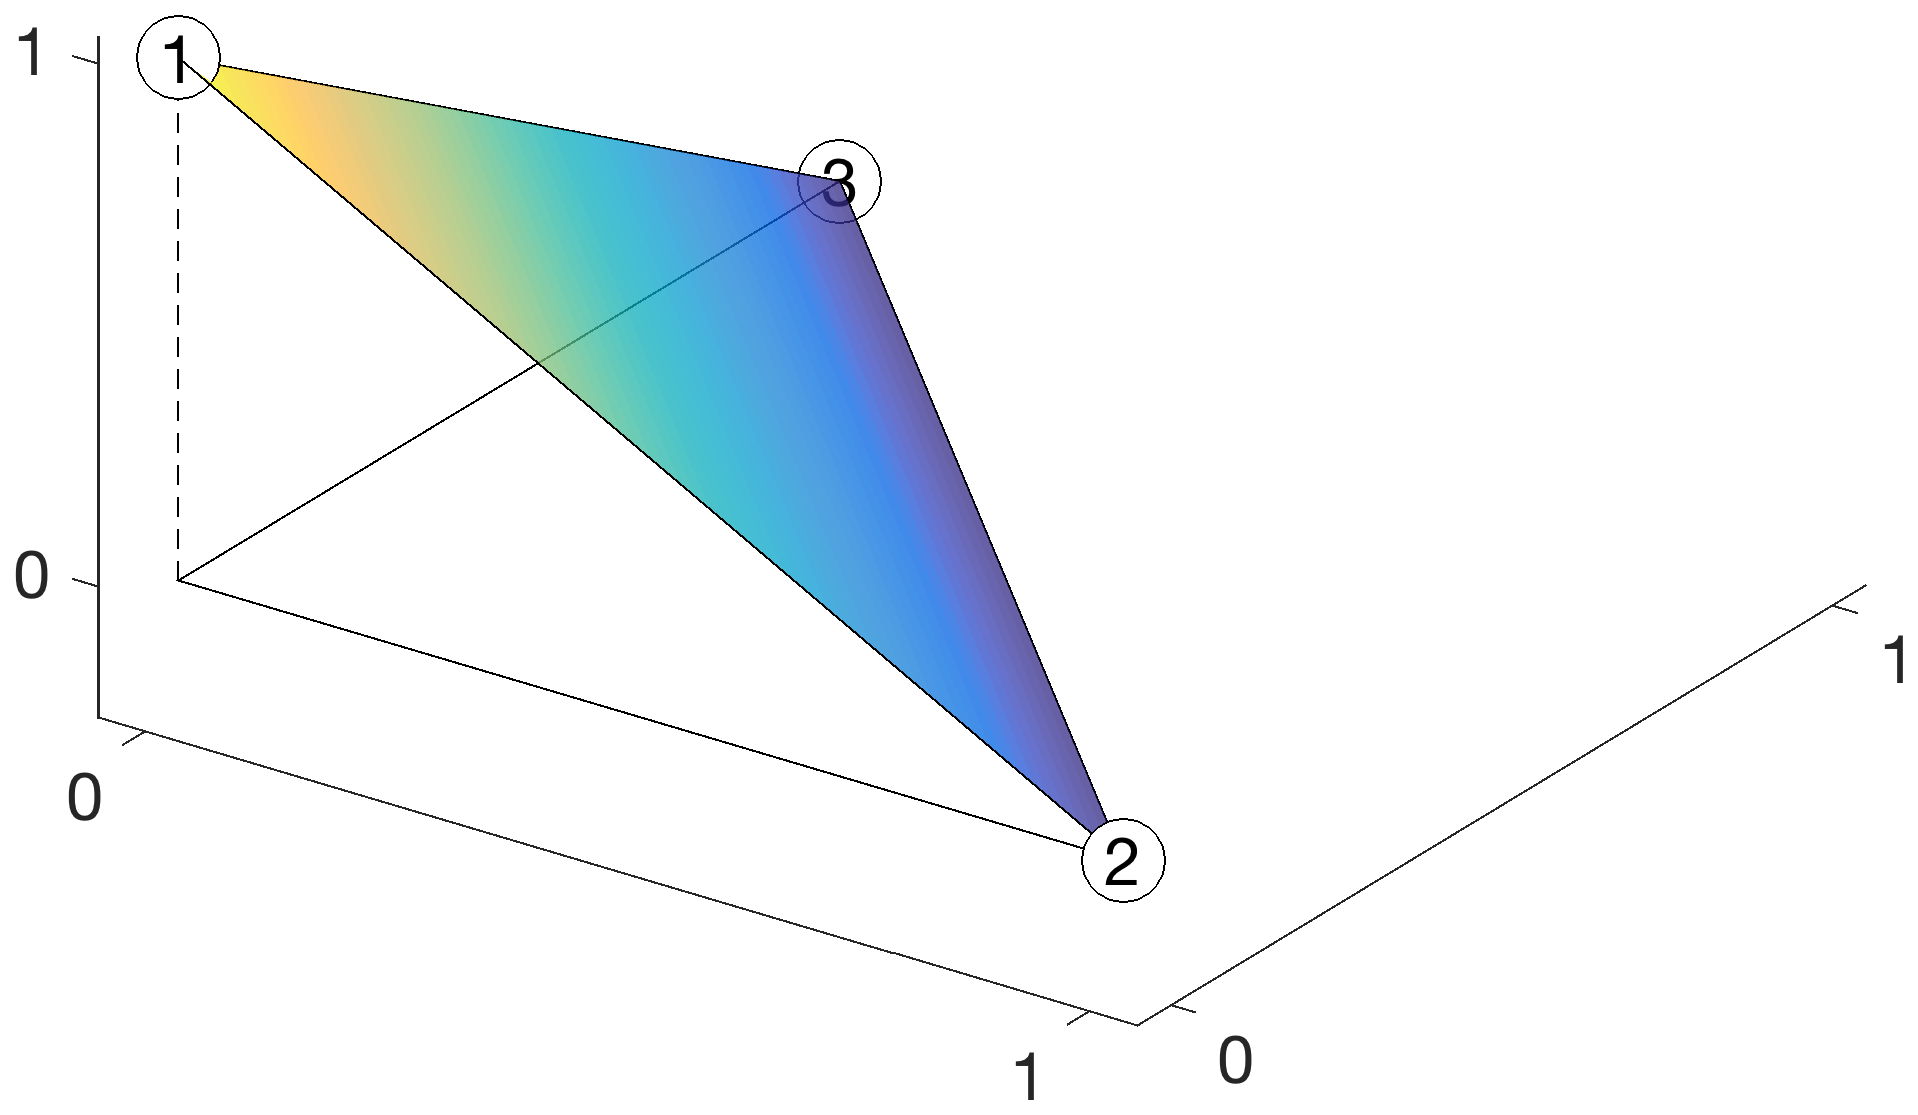
\includegraphics[width=0.3\textwidth]{shape_tri_p1_1}
  }
  \subfigure[$\tilde \phi_2$]{
    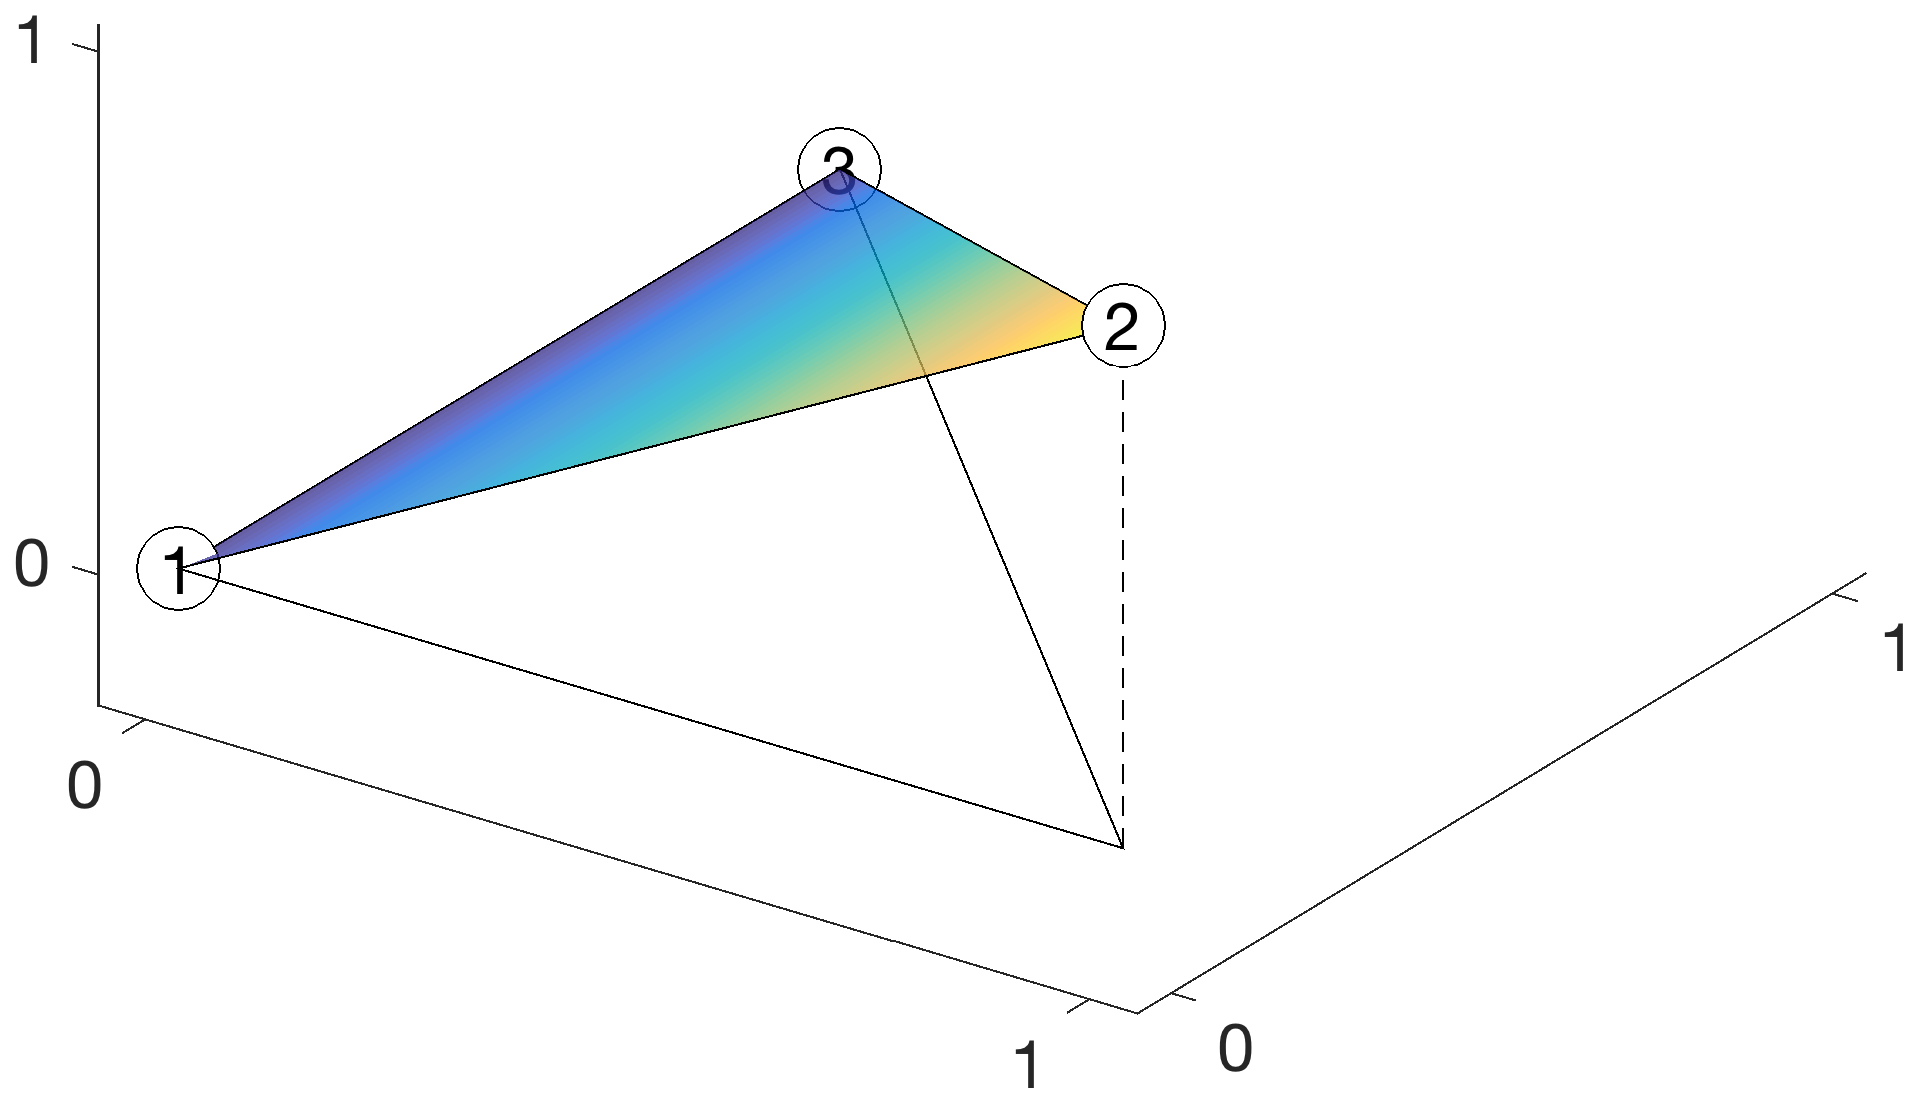
\includegraphics[width=0.3\textwidth]{shape_tri_p1_2}
  }
  \subfigure[$\tilde \phi_3$]{
    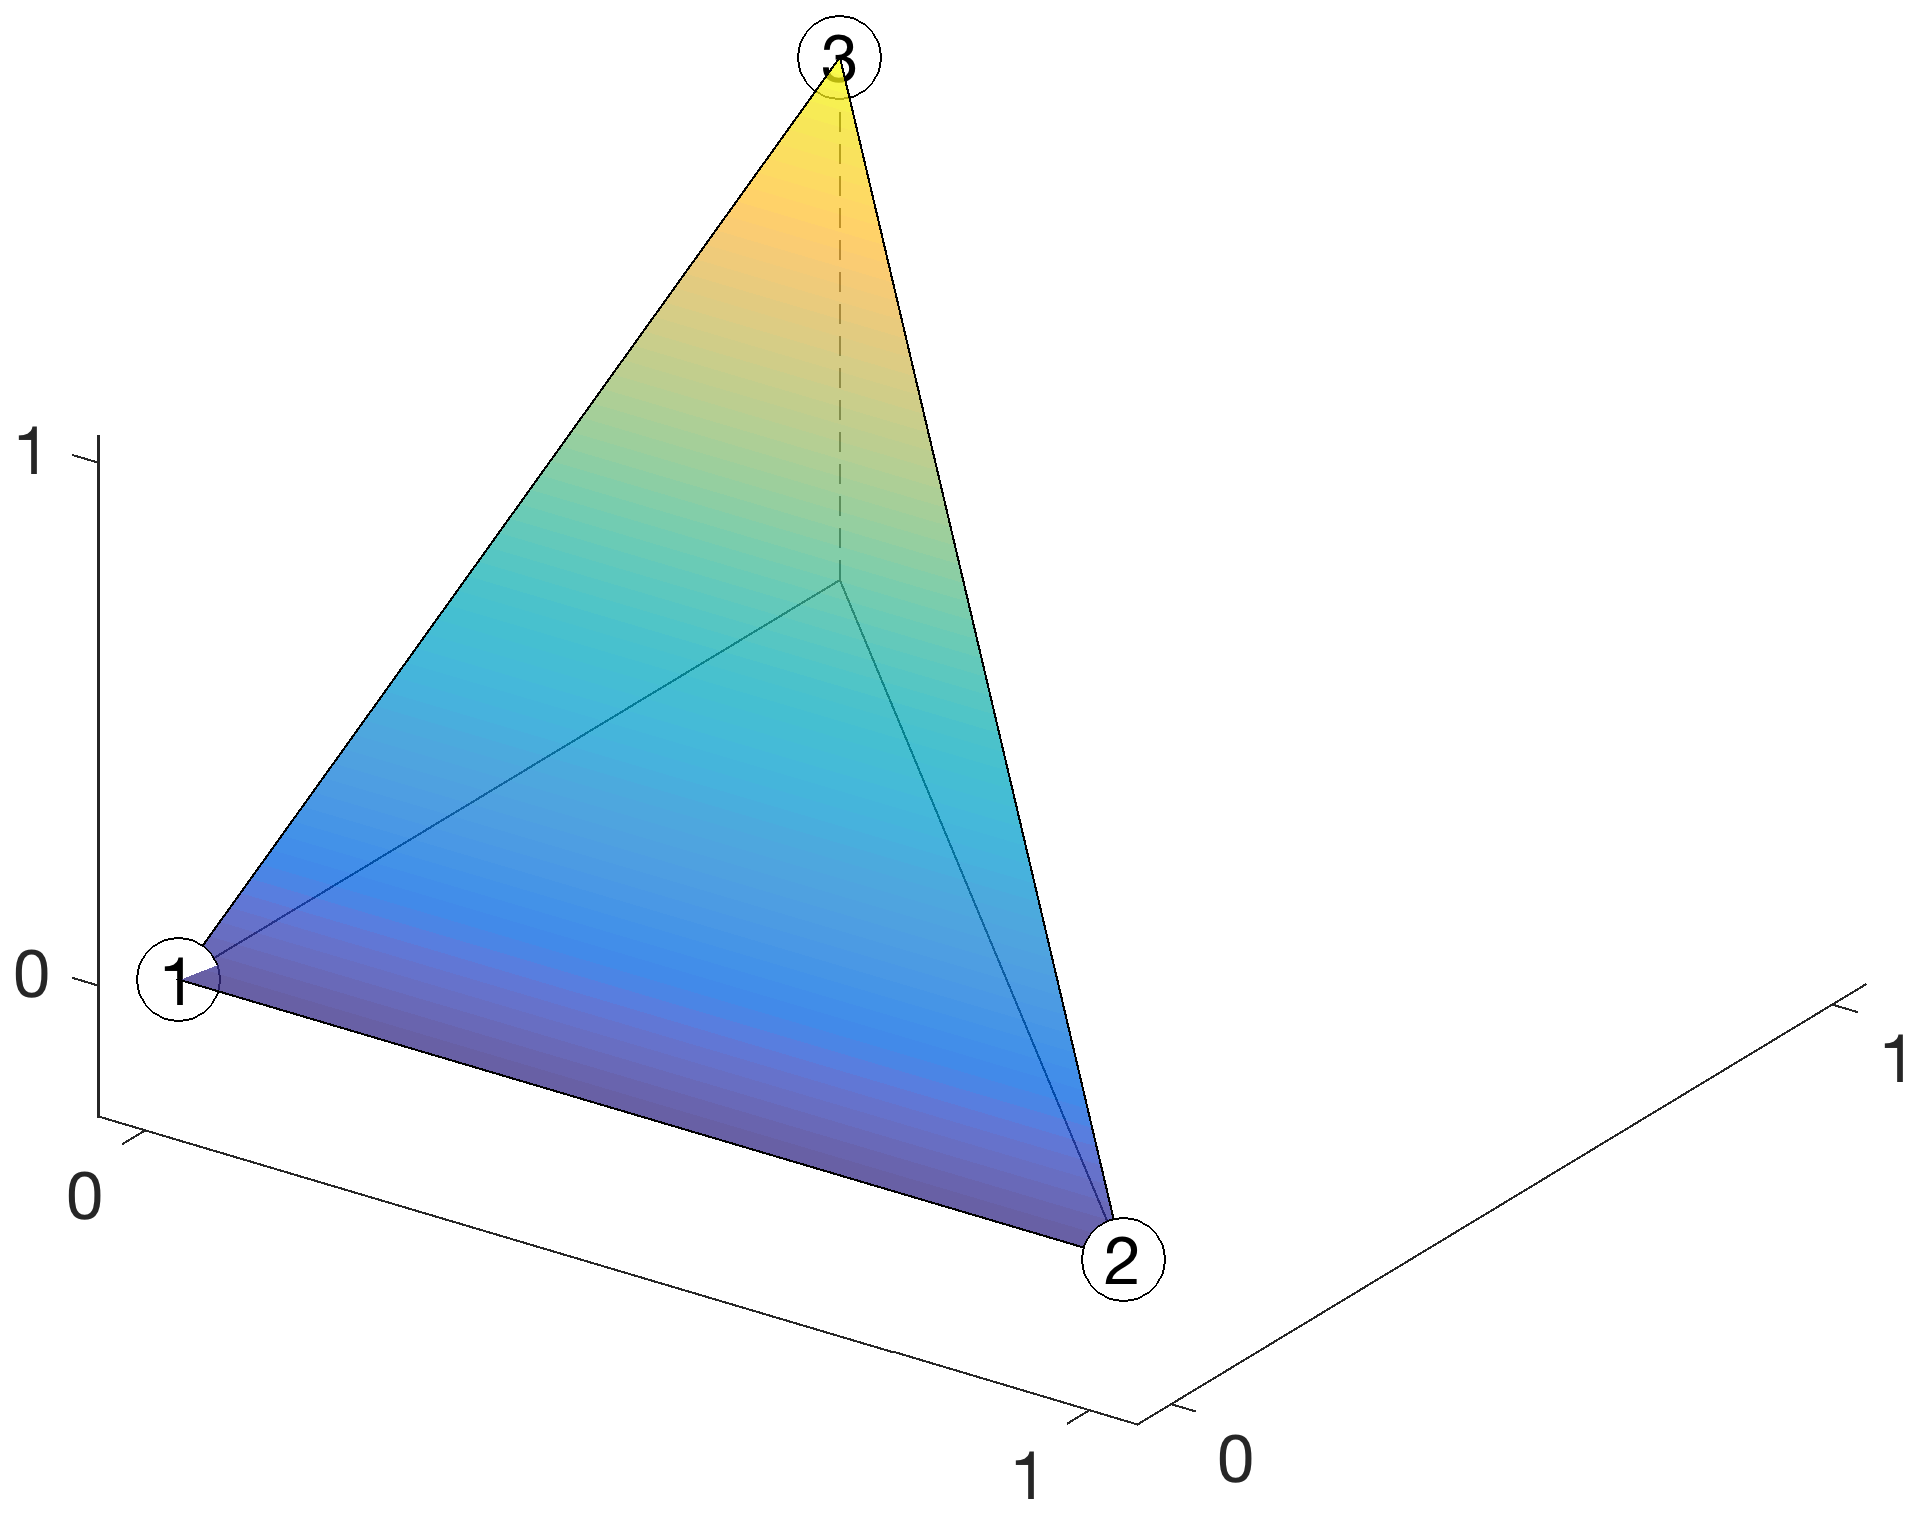
\includegraphics[width=0.3\textwidth]{shape_tri_p1_3}
  }
  \caption{Linear Lagrange shape functions on the reference triangle.}
  \label{fig:fe_shape_tri_p1}
\end{figure}

Once we find the coefficients of the shape functions, we can evaluate the value of the functions at any point in the triangle by evaluating~\eqref{eq:fe_lin_tri_rep}. We can also differentiate~\eqref{eq:fe_lin_tri_rep} to obtain the gradient of the shape functions:
\begin{align*}
  \pp{\tilde \phi_j}{\tilde x_1}(x) = a_2^{(j)}
  \quad \text{and} \quad
  \pp{\tilde \phi_j}{\tilde x_2}(x) = a_3^{(j)}, \quad j = 1,2,3.
\end{align*}
For the linear Lagrange element, the derivatives are constant over the element because the shape functions are linear.

Using the linear Lagrange basis functions, we can now represent any function $v$ that is in $\PP^1(\tilde K)$.  Specifically, we may represent $v \in \PP^1(\tilde K)$ in terms of a coefficient vector $\hat v \in \RR^3$ as
\begin{equation*}
  v(\tilde x) = \sum_{j=1}^{3} \hat v_j  \tilde \phi_j(\tilde x) \quad \forall \tilde x \in \tilde K
\end{equation*}
for $\hat v_j \equiv v(\tilde x^j)$, $j = 1,2,3$.  We hence have a one-to-one mapping between \emph{any} element in $\PP^1(\tilde K)$ and the associated coefficient vector in $\RR^3$.  For the linear Lagrange basis functions, the coefficients $\hat v \in \RR^3$ is associated with the values of the function at the vertices of the triangle.

Before we introduce other finite elements, we use the linear Lagrange element as an example to describe three properties that formally defines a \emph{finite element}:
\begin{enumerate}
\item the domain $\tilde K$ over which the element is defined; e.g., the reference triangle $\tilde K$ defined by vertices shown in Figure~\ref{fig:fe_ref_tri}.
\item the finite-dimensional linear space of functions; e.g., the linear polynomial space $\PP^1(\tilde K)$ spanned by $\{ 1, \tilde x_1, \tilde x_2 \}$.
\item the degree of freedom used to describe functions; e.g., the values of the function at the vertices of the triangle.
\end{enumerate}

\section{Isoparametric mapping}
In Section~\ref{sec:fe_lin_tri}, we introduced a linear finite element associated with a reference triangle.  We now wish to map the finite element to a physical element that constitutes the triangulation $\calT_h$.  To this end, we introduce the procedure based on \emph{isoparametric mapping}.

\begin{figure}
  \centering
  \subfigure[reference element]{
    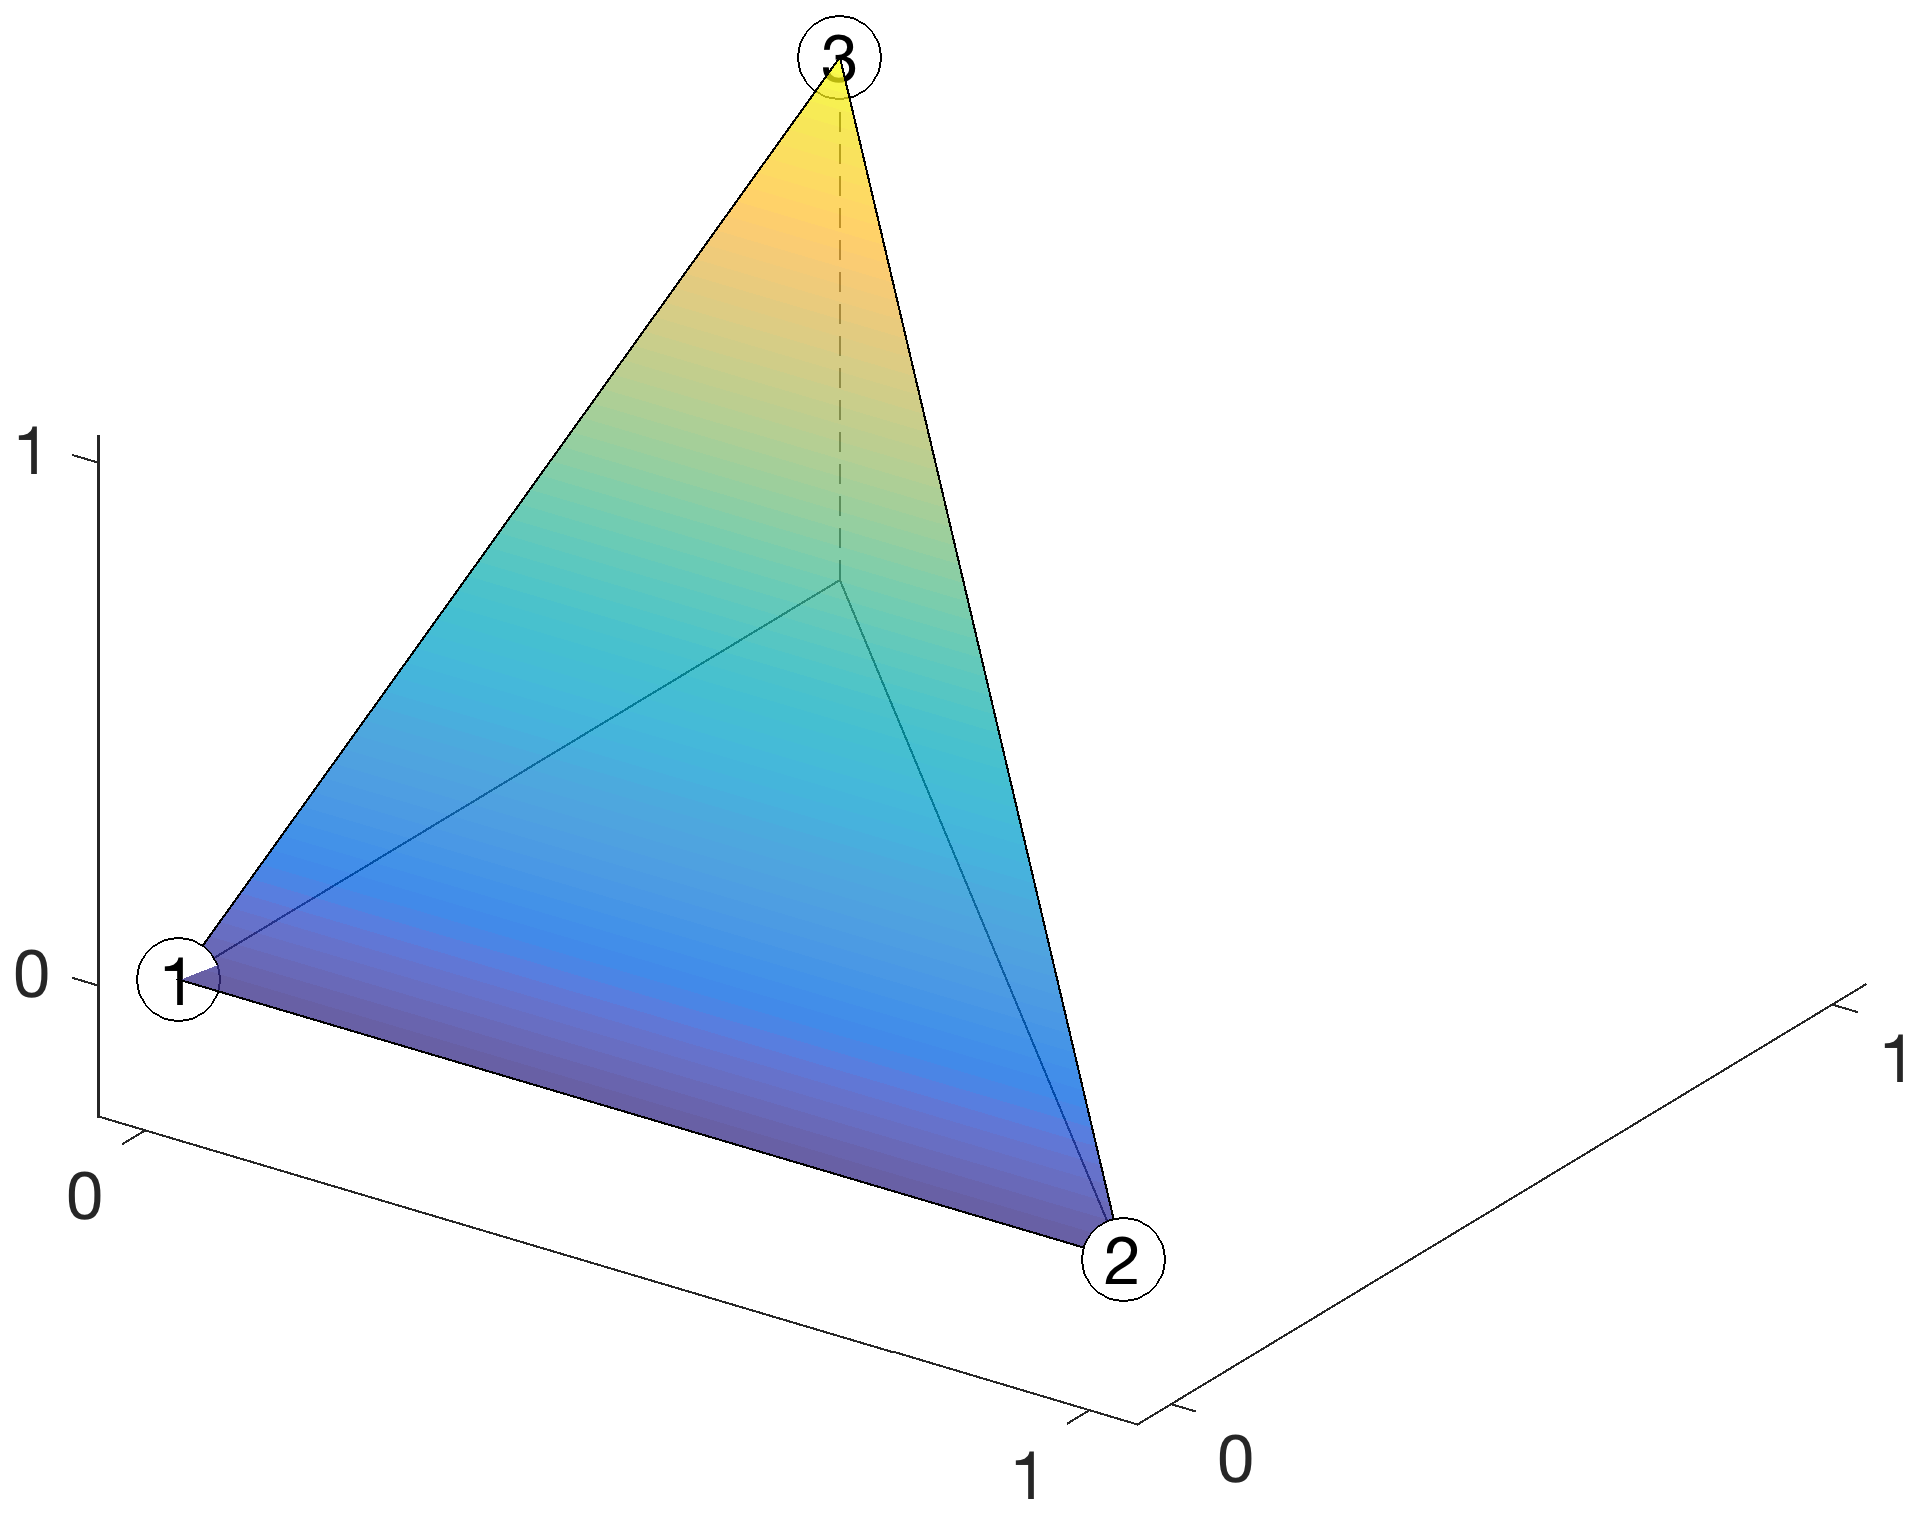
\includegraphics[width=0.3\textwidth]{shape_tri_p1_3}
  }
  \subfigure[physical element]{
    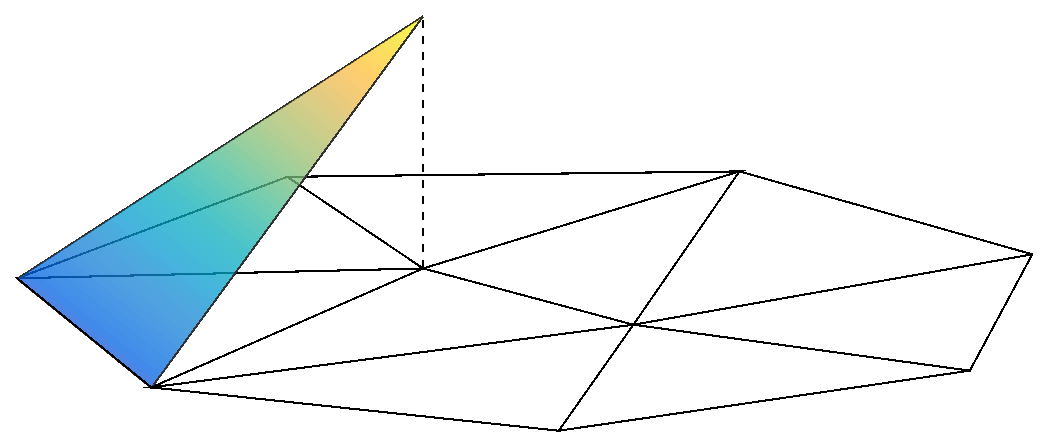
\includegraphics[width=0.4\textwidth]{shape_global_p1_part}
  }
\end{figure}

The isoparametric mapping is a mapping from the reference element to the physical element such that (i) the mapping is polynomial and (ii) the Lagrange interpolation points of the reference element are mapped to the respective Lagrange interpolation points of the physical element. For instance, for a linear triangle, the mapping is linear and vertices of the reference triangle are mapped to the respective vertices of the physical triangle.   Algebraically, the isoparametric mapping that maps $\xi \in \tilde K$ to $x \in K$ is given by
\begin{equation}
  x_i(\xi) = \sum_{j=1}^{n_s} x^j_i \tilde \phi_j(\xi), \quad i = 1,\dots,d,
  \label{eq:fe_iso_map}
\end{equation}
where $x_i^j$ is the $i$-th coordinate of the $j$-th interpolation point, and $\tilde \phi_i$ is the Lagrange basis function on the reference element associated with the $i$-th interpolation node, and $n_s$ is the number of basis functions, which is equal to the number of interpolation points.
As a concrete example, consider the triangulation shown in Figure~\ref{fig:fe_mesh_p1} (and encoded in Table~\ref{tb:fe_mesh_p1}).  For the physical element 7, we have
\begin{equation*}
  x^1 = v^7 = (0.33,0.66), \quad 
  x^2 = v^8 = (0.43,0.31), \quad \text{and} \quad
  x^3 = v^{11} = (0.68,0.58);
\end{equation*}
the associated basis functions are given by~\eqref{eq:fe_lin_tri_expl}.
The map~\eqref{eq:fe_iso_map} satisfies the two conditions of isoparametric mapping:
\begin{itemize}
\item[(i)] Because the Lagrange basis functions are polynomial, the mapping $\xi \mapsto x$ is polynomial.
\item[(ii)] The $k$-th interpolation point of the reference triangle $\xi^k$ is mapped to the $k$-th interpolation point of the physical triangle $x^k$ since $x(\xi^k) = \sum_{j=1}^{n_s} x^j \tilde \phi_j(\xi^k) = \sum_{j=1}^{n_s} x^j \delta_{jk} = x^k$.
\end{itemize}
Hence, $\tilde K \ni \xi \mapsto x \in K$ is an isoparametric mapping.

With this mapping, we can now construct 

\begin{figure}
  \centering
  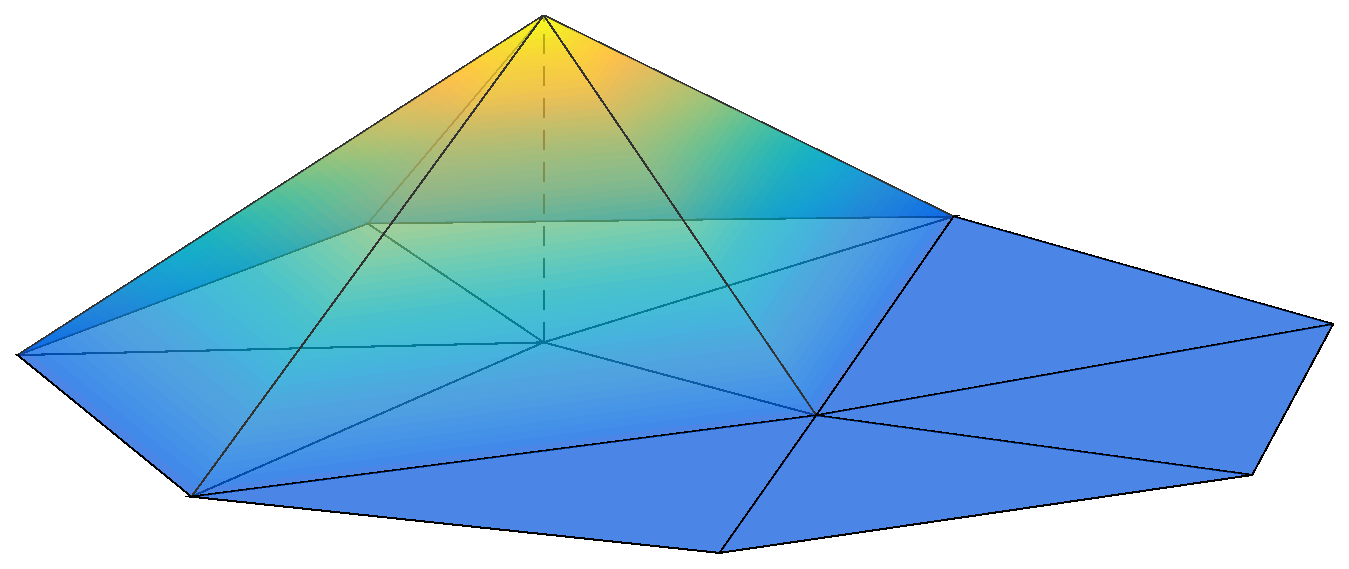
\includegraphics[width=0.48\textwidth]{shape_global_p1}
\end{figure}


We can differentiate~\eqref{eq:fe_iso_map} to evaluate the \emph{Jacobian} of the isoparametric mapping; the $(i,j)$ entry of the Jacobian $J \equiv \pp{x}{\xi_j} \in \RR^{d \times d}$, is given by
\begin{equation*}
  J_{ij} = \pp{x_i}{\tilde x_j} = \sum_{j=1}^{n_s} x^j_i \pp{\tilde \phi_i}{\tilde x_j} .
\end{equation*}

\begin{equation*}
  dx = \text{det}(J) d\tilde x
\end{equation*}

\begin{equation*}
  \pp{\xi}{x} = \left( \pp{x}{\xi} \right)^{-1}
\end{equation*}

\begin{equation*}
  \phi(x) = \tilde \phi (\xi)
\end{equation*}

\begin{equation*}
  \pp{\phi}{x_i}(x) = \left. \pp{\tilde \phi}{\xi_j} \right|_\xi  \left. \pp{\xi_j}{x_i} \right|_\xi
\end{equation*}



For a quadratic triangle, the mapping is quadratic and vertices and mid-edge nodes of the reference triangle are mapped to the respective vertices and mid-edge nodes of the physical triangle.

Formally, a finite element space is parametrized by the following three properties:
\begin{enumerate}
\item the triangulation $\calT_h$ of $\Omega$;
\item the type of functions that constitutes the space (e.g., piecewise linear polynomial);
\item the degrees of freedom used to describe functions in the space.
\end{enumerate}
The first two are apparent from the definition of the finite element space~\eqref{eq:fe_space}.  The last property determines how a function $v \in \calV_h$ is represented on a computer.  Specifically, given a $N$-dimensional function space $\calV_h$, we assign $N$ degrees of --- by choosing $N$ basis functions --- such that the a function $v \in \calV_h$ can be uniquely described by $N$ real numbers.  We will clarify this third property in Section~\ref{sec:fe_map}.

\section{Quadratic Lagrange finite element on a triangle}
We now introduce a quadratic Lagrange finite element on a triangle. A quadratic function in $\PP^2(\tilde K)$ takes on the form $a_1 + a_2 \tilde x_1 + a_3 \tilde x_2 + a_4 \tilde x_1^2 + a_5 \tilde x_1 \tilde x_2 + a_6 \tilde x_2^2$ and ahs six degrees of freedom; we hence wish to identify a linearly independently set of six quadratic Lagrange basis functions.  To this end, we choose for our Lagrange interpolation nodes the three vertices of the triangle and three points at the middle of the edges
\begin{equation*}
  x^{(1)} = (0,0), \quad x^{(2)} = (1,0), \quad x^{(3)} = (0,1), \quad x^{(4)} = (1/2,1/2), \quad x^{(5)} = (0,1/2), \quad x^{(6)} = (1/2,0),
\end{equation*}
as shown in Figure~\ref{fig:fe_ref_tri_p2}.  The ordering of the quadratic nodes is not universal in the finite element literature; we here adhere the convention that, for $i \in \{4,5,6\}$, the $i$-th node is on the midpoint of the $i-3$-th edge of the reference triangle. Our goal is to find the Lagrange basis functions $\{\tilde \phi_i\}_{i=1}^6$ that lie in the $\PP^2(\tilde K)$ space and satisfy the interpolation condition $\tilde \phi_i(\tilde x^{(j)}) = \delta_{ij}$.

\begin{figure}
  \centering
  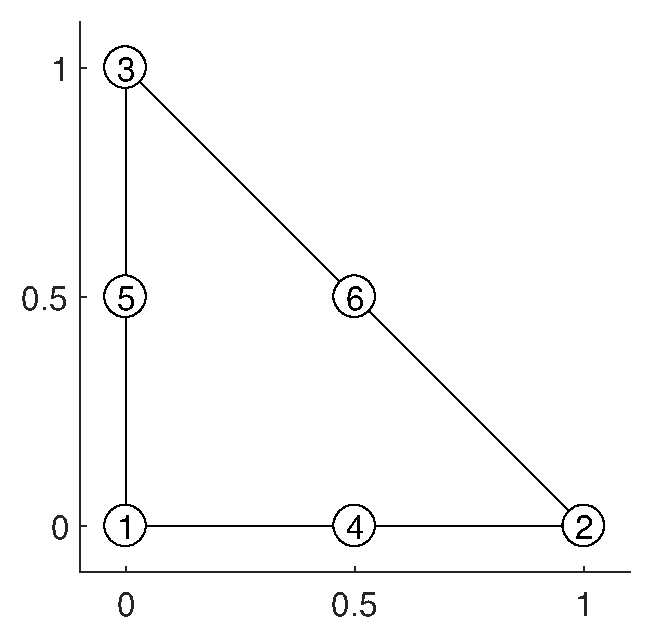
\includegraphics[width=0.3\textwidth]{ref_tri_p2}
  \caption{Quadratic Lagrange finite element on the reference triangle.}
  \label{fig:fe_ref_tri_p2}
\end{figure}


We now employ the procedure used in Section~\ref{sec:fe_lin_tri} to generate the quadratic Lagrange basis. We first express the basis functions in terms of the monomial basis
\begin{equation}
  \tilde \phi_j(\tilde x) = a_1^{(j)} + a_2^{(j)} \tilde x_1 + a_3^{(j)} \tilde x_2 + a_4^{(j)} \tilde x_1^2 + a_5^{(j)} \tilde x_1 \tilde x_2 + a_6^{(j)} \tilde x_2^2 \quad j = 1,\dots,6;
  \label{eq:fe_quad_tri_rep}
\end{equation}
we then express the interpolation condition $\tilde \phi_i(\tilde x^{(j)}) = \delta_{ij}$ as a $6 \times 6$ matrix system
\begin{equation*}
  V A = I,
\end{equation*}
where $A_{ij} = a^{(j)}_i$, $i,j = 1,\dots,6$, and the $i$-th row of the Vandermonde matrix $V \in \RR^{6 \times 6}$ is
\begin{equation*}
  V_{i:} = \bmat{cccccc} 1 & \tilde x^{(i)}_1 & \tilde x^{(i)}_2 &  (\tilde x^{(i)}_1)^2 & \tilde x^{(i)}_1 \tilde x^{(i)}_2 & (\tilde x^{(i)}_2)^2 \emat .
\end{equation*}
The linear system has a unique solution.  Figure~\ref{fig:fe_shape_tri_p2} shows the six basis functions.

\begin{figure}
  \centering
  \subfigure[$\tilde \phi_1$]{
    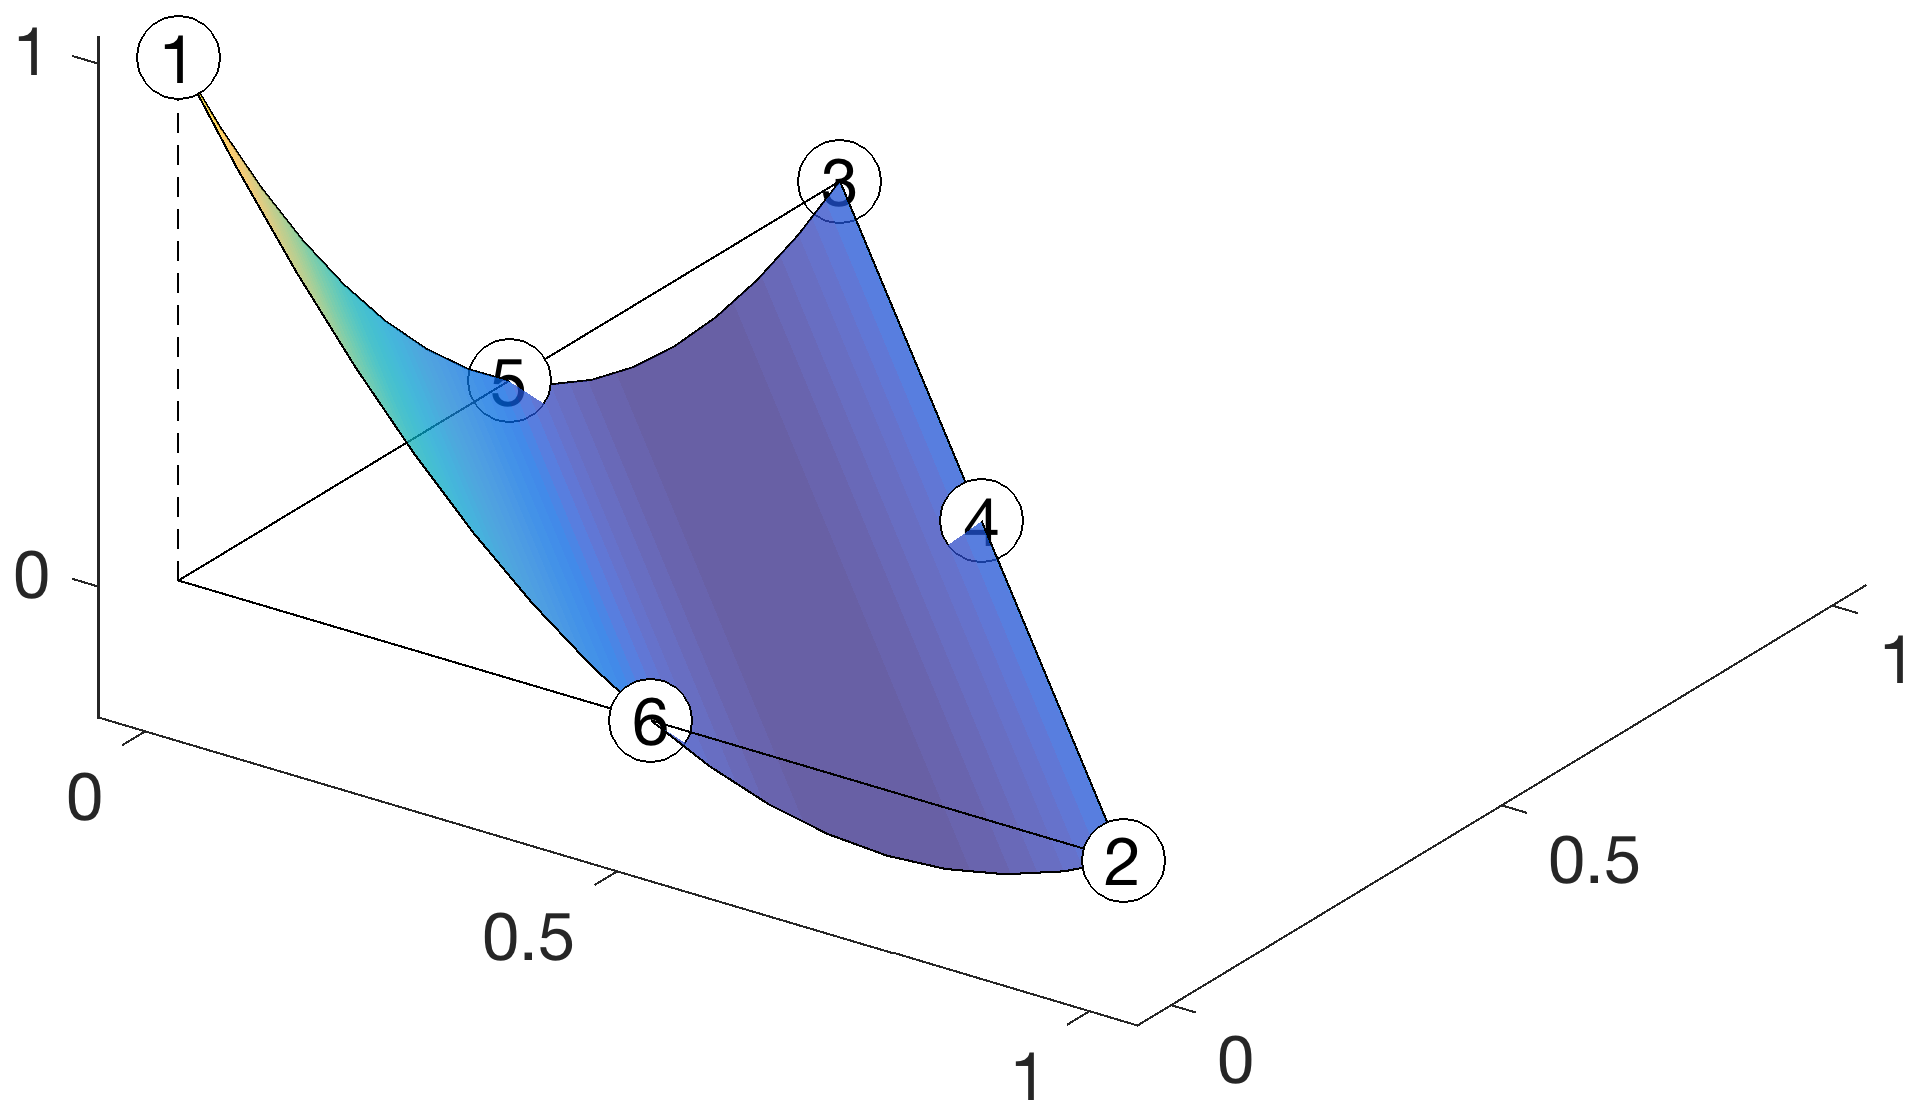
\includegraphics[width=0.3\textwidth]{shape_tri_p2_1}
  }
  \subfigure[$\tilde \phi_2$]{
    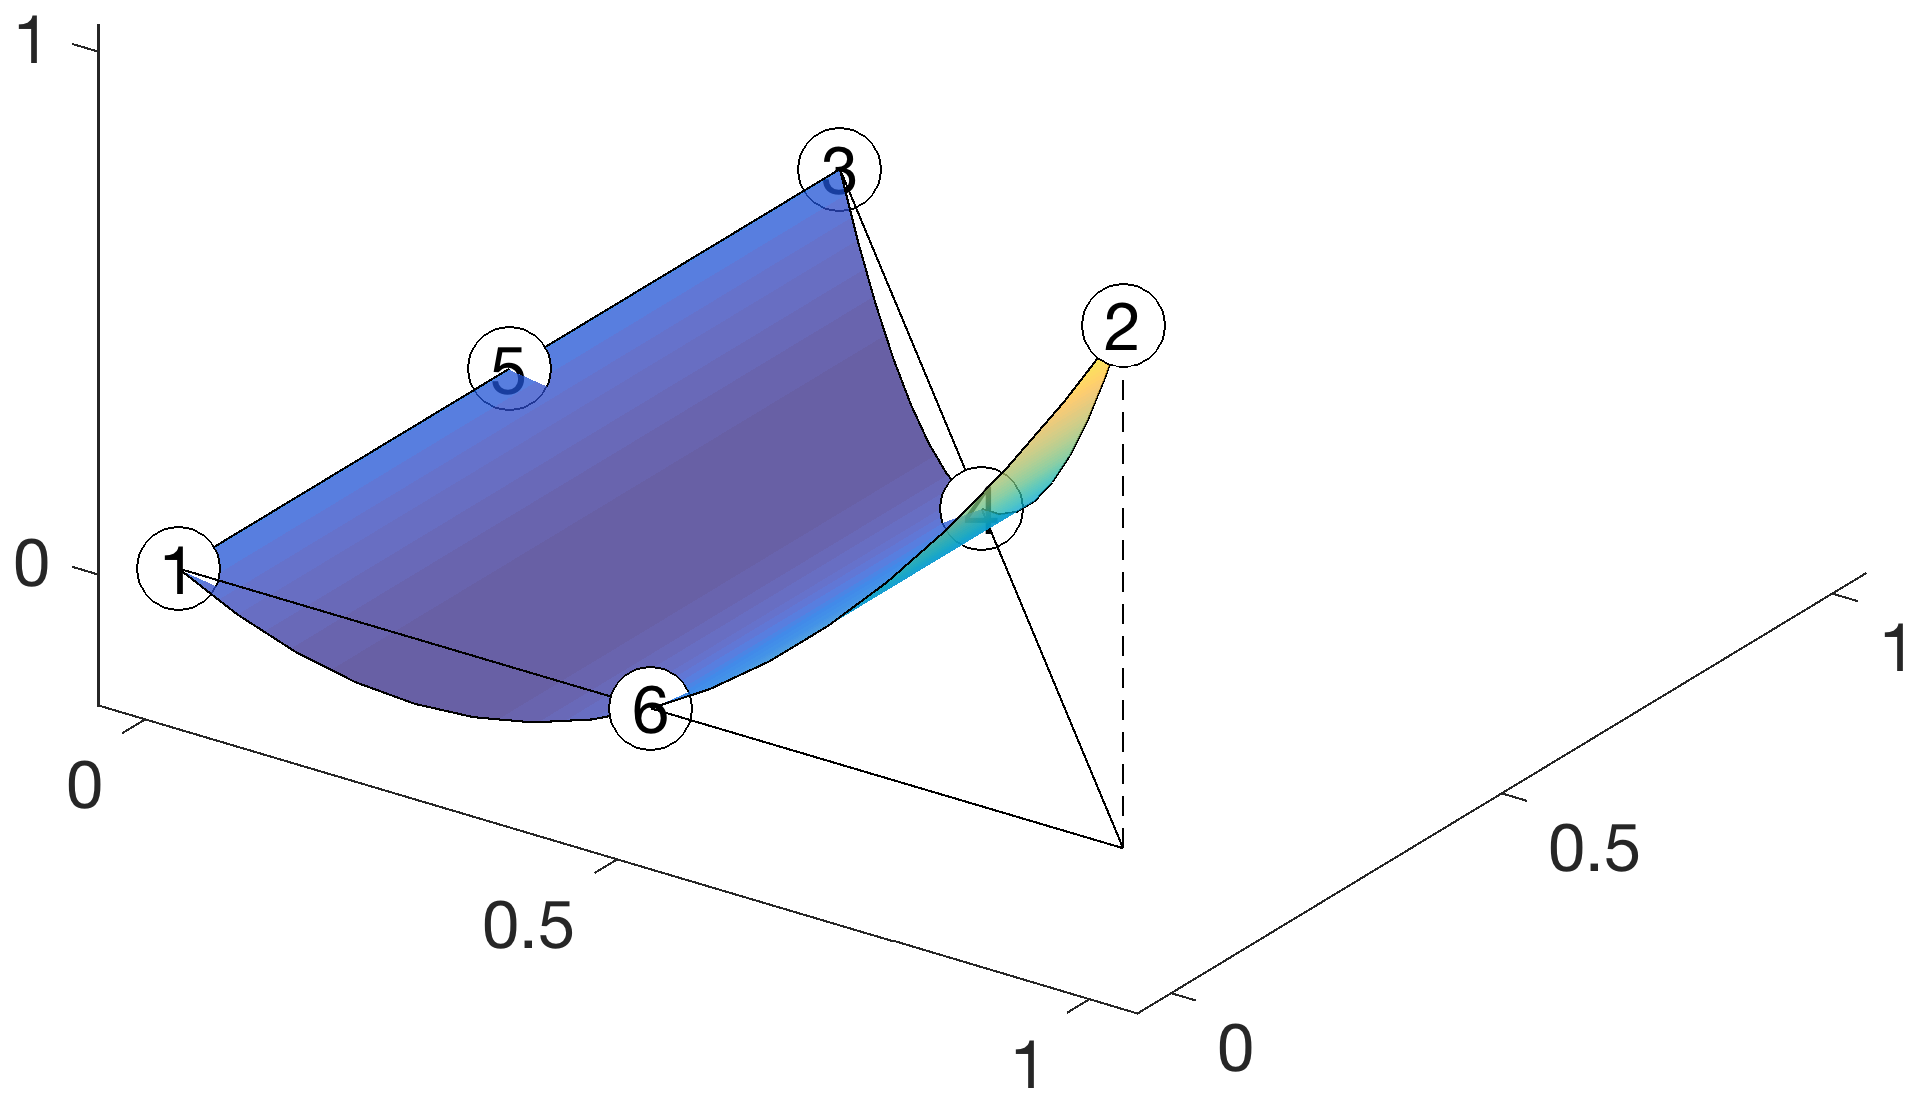
\includegraphics[width=0.3\textwidth]{shape_tri_p2_2}
  }
  \subfigure[$\tilde \phi_3$]{
    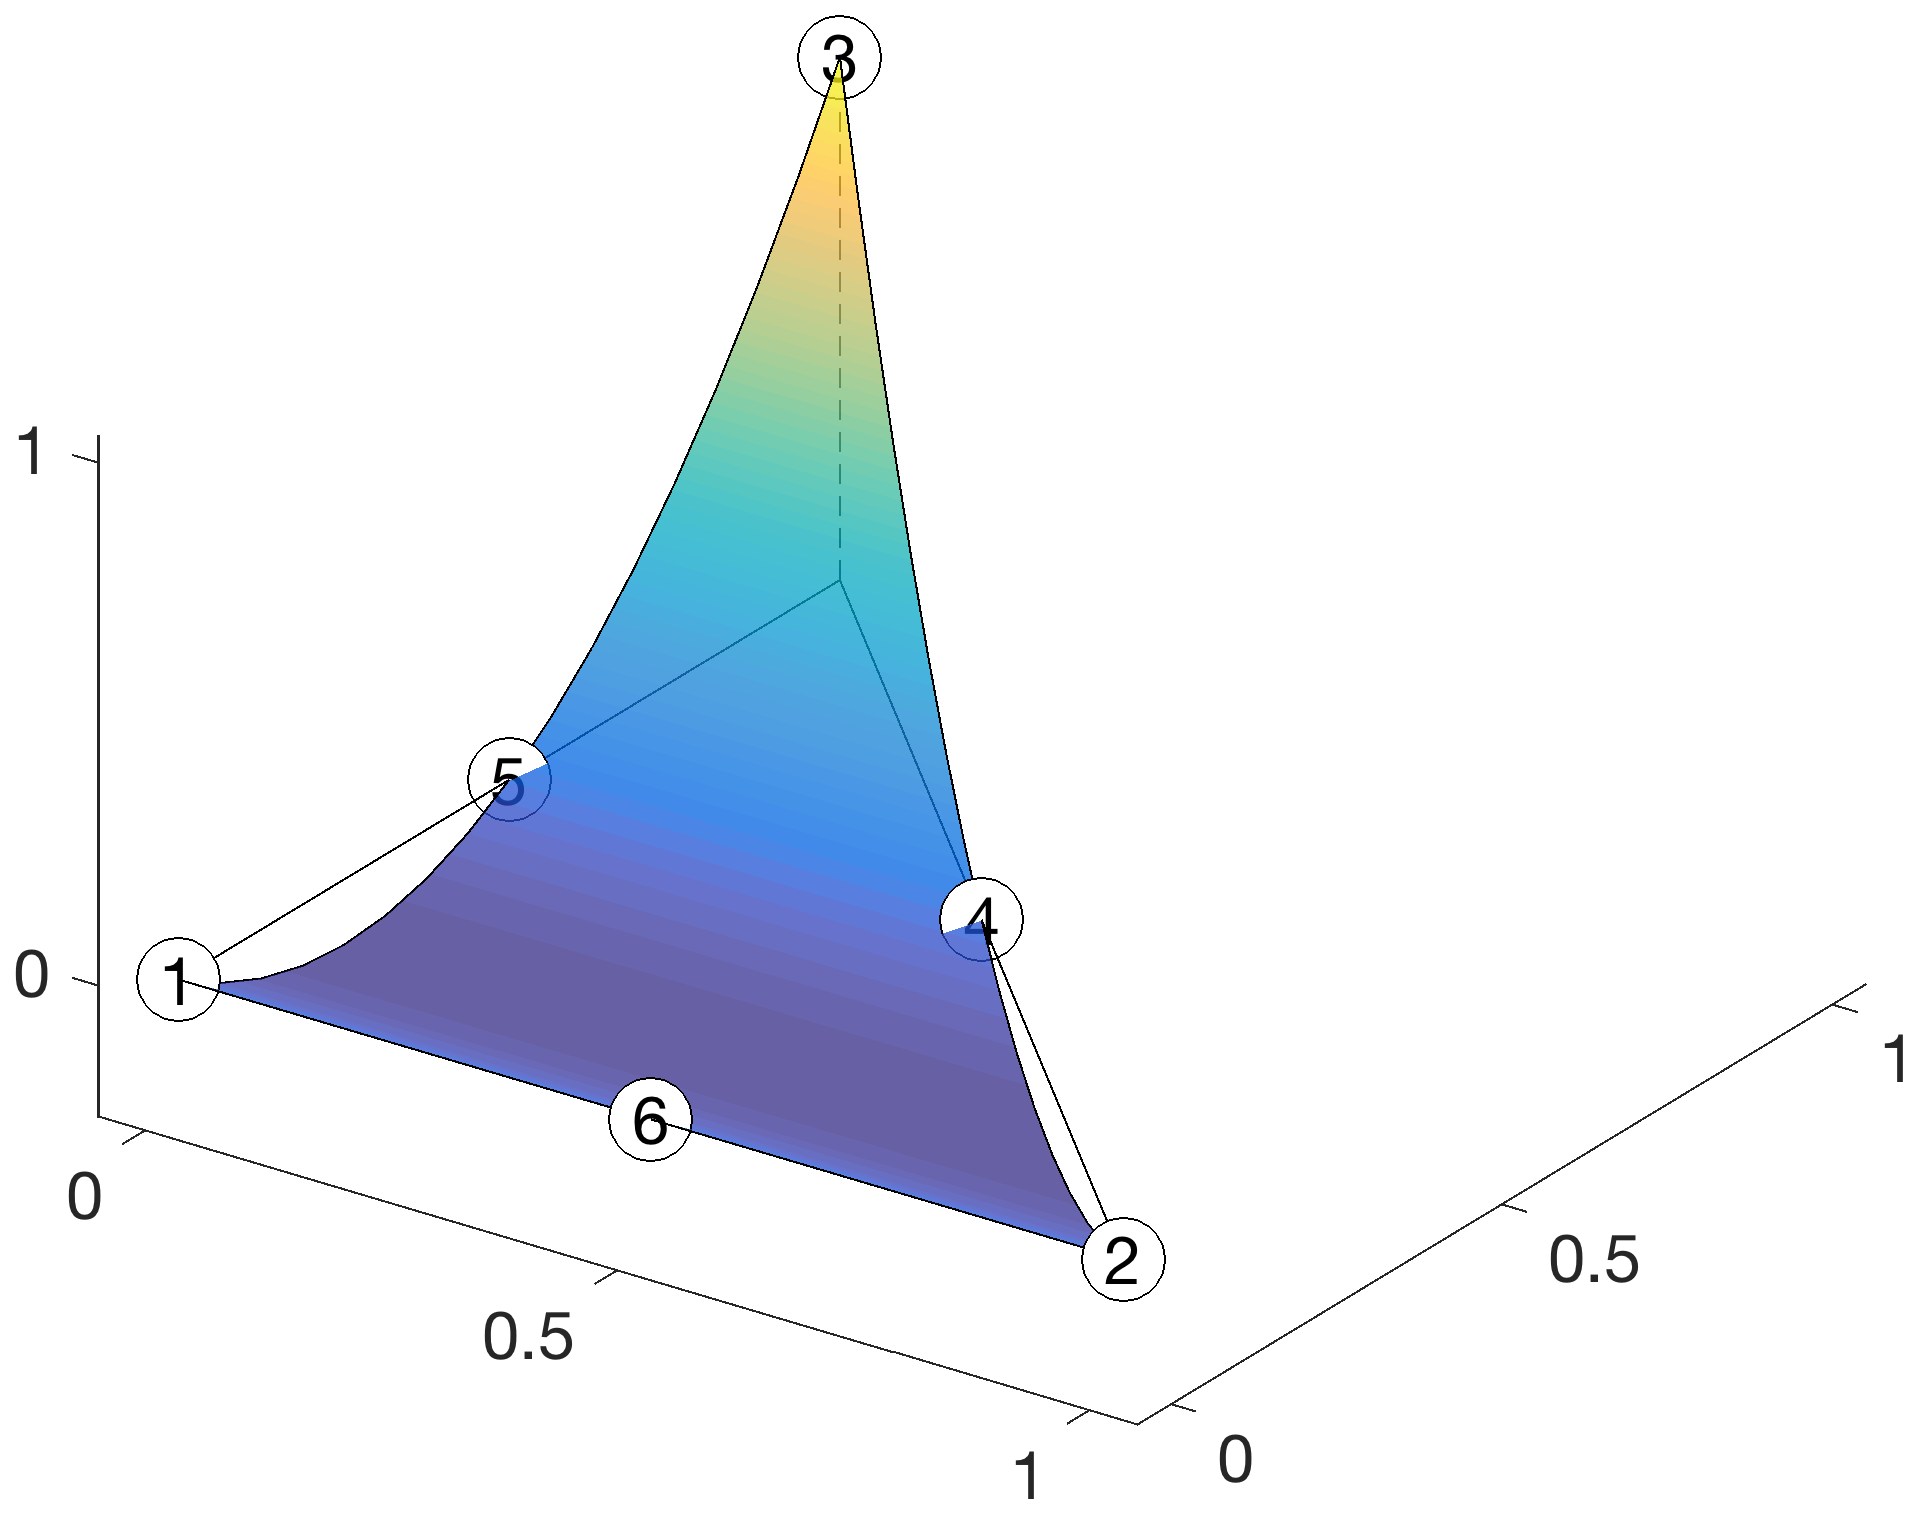
\includegraphics[width=0.3\textwidth]{shape_tri_p2_3}
  }
  \subfigure[$\tilde \phi_4$]{
    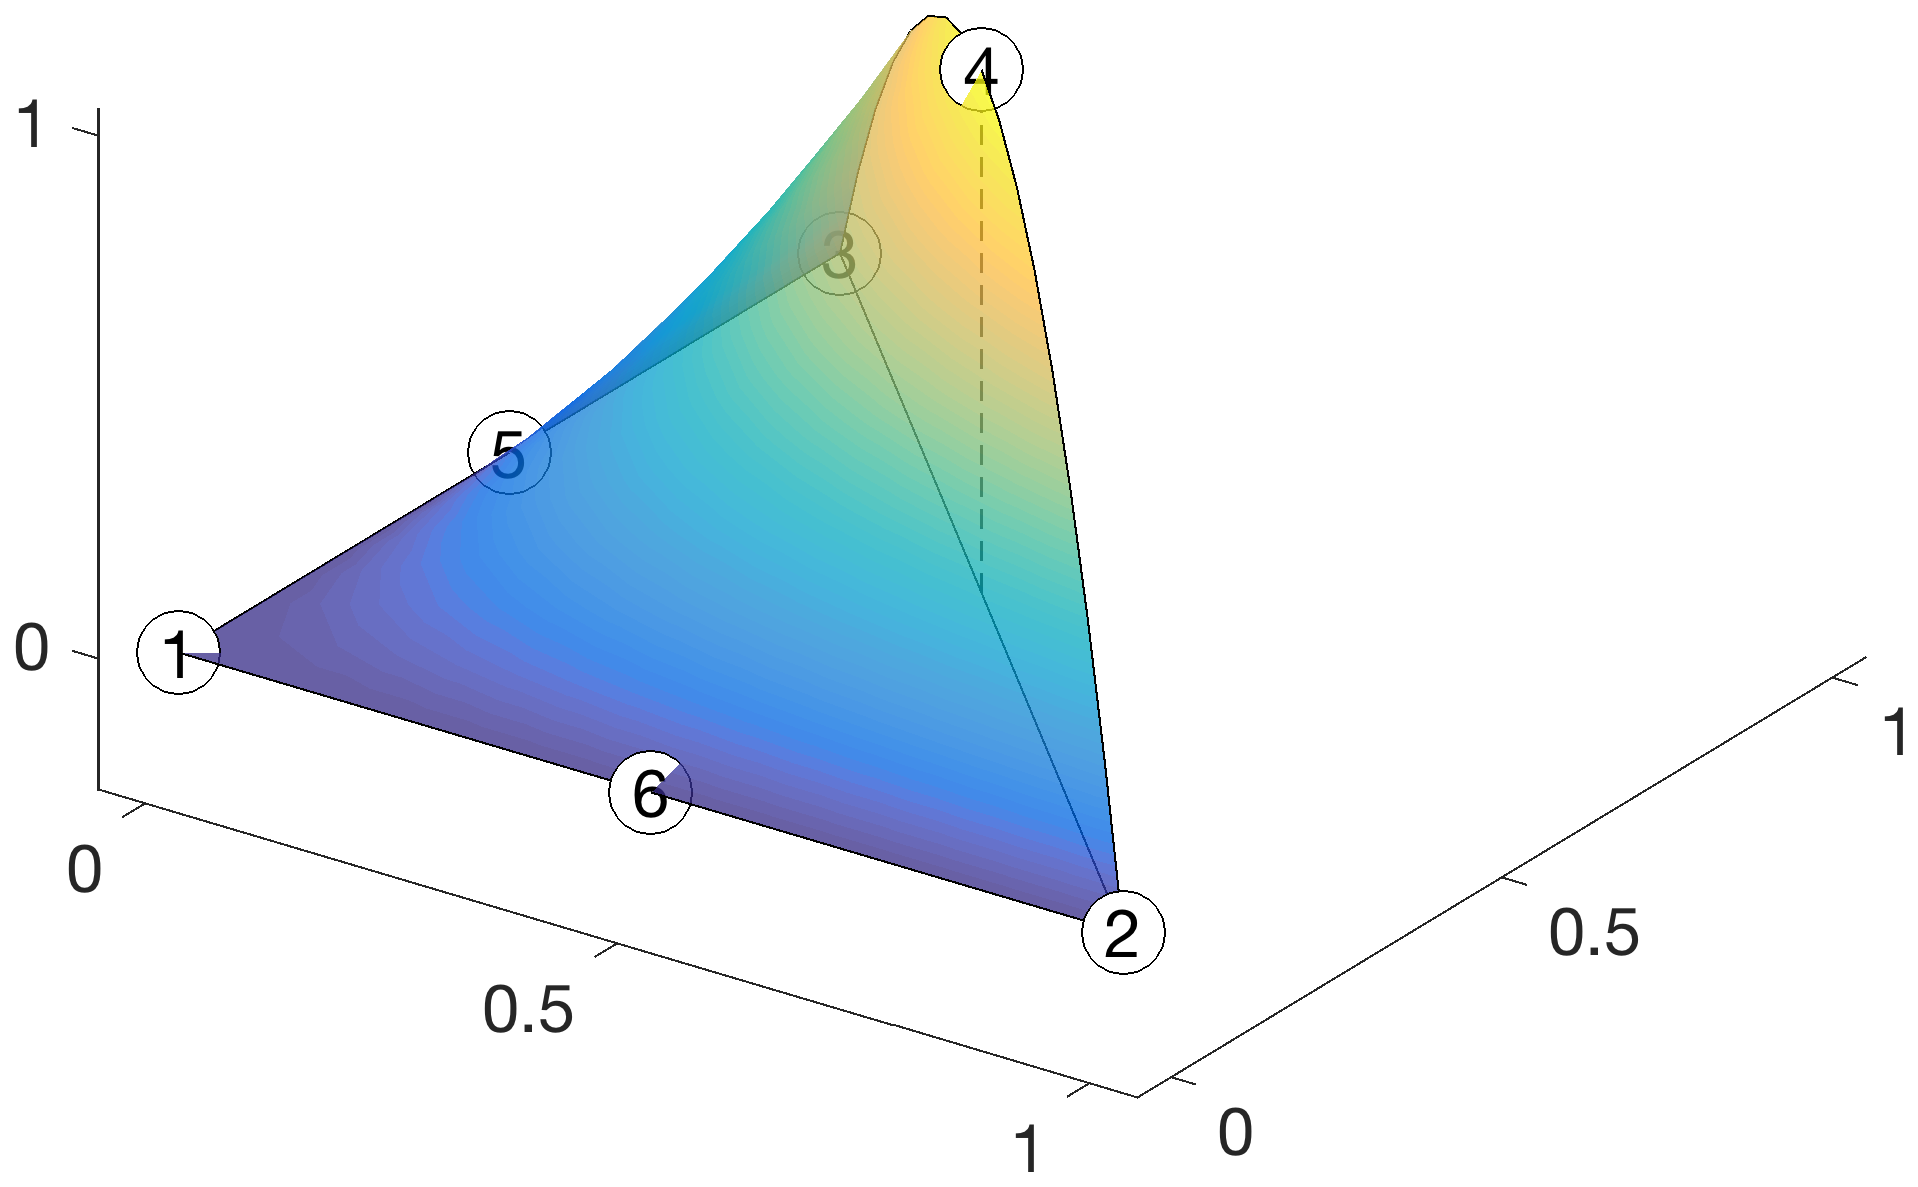
\includegraphics[width=0.3\textwidth]{shape_tri_p2_4}
  }
  \subfigure[$\tilde \phi_5$]{
    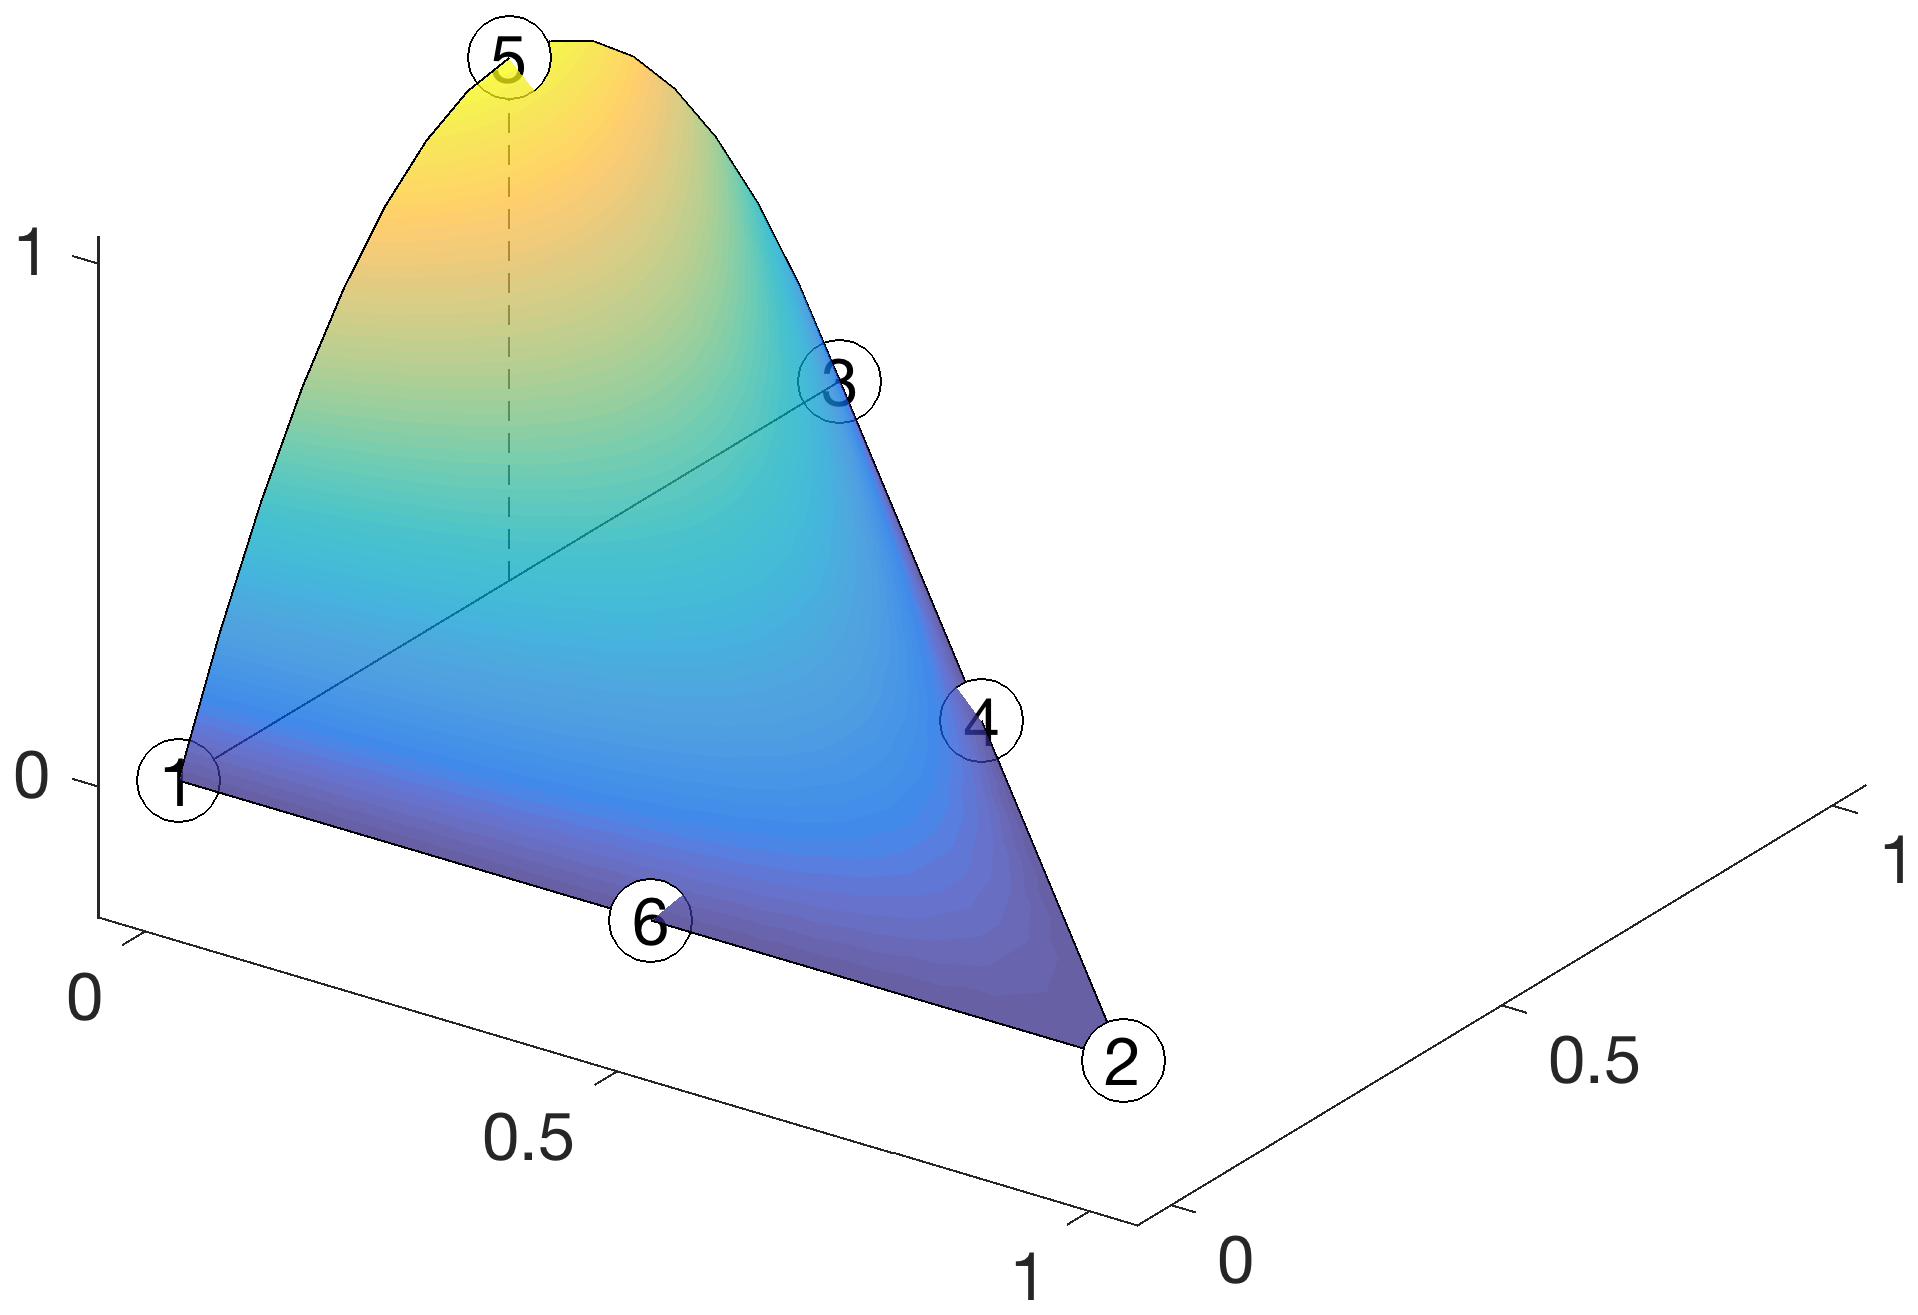
\includegraphics[width=0.3\textwidth]{shape_tri_p2_5}
  }
  \subfigure[$\tilde \phi_6$]{
    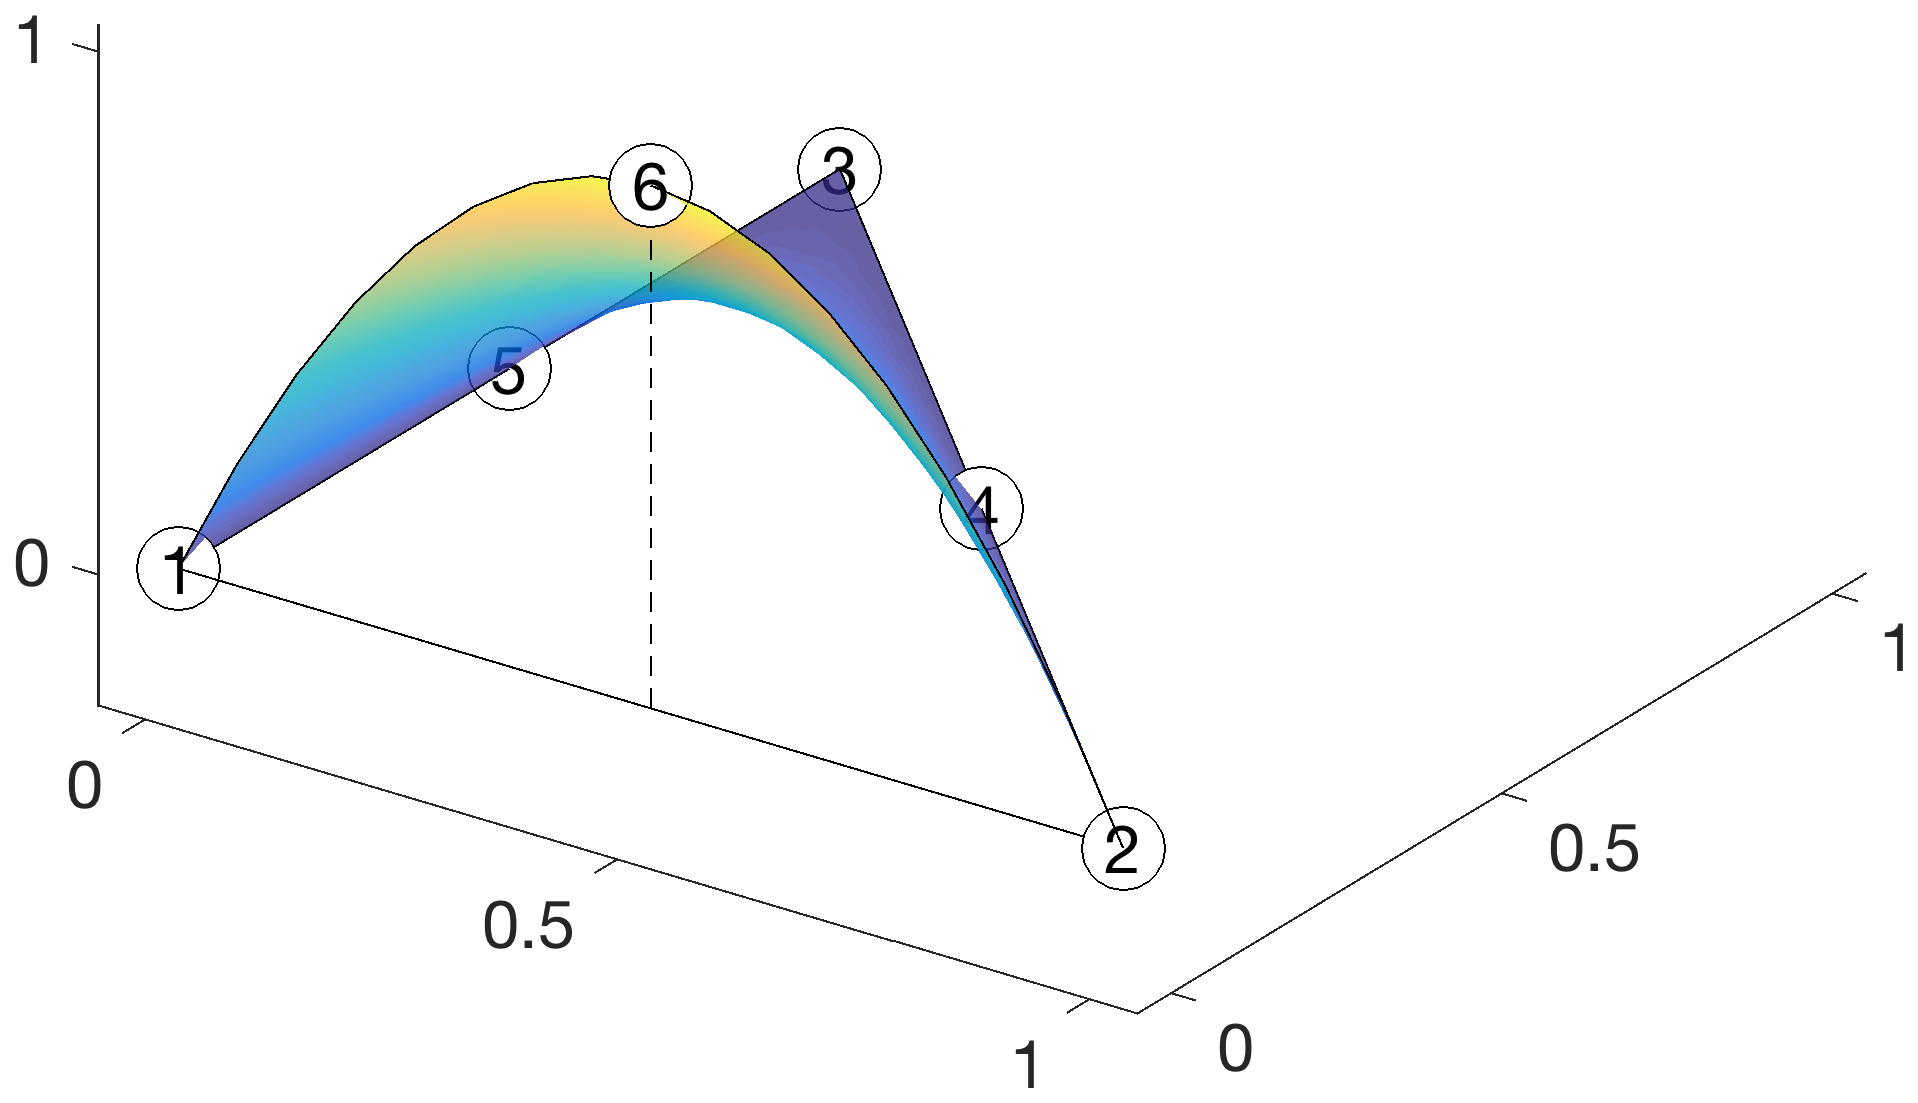
\includegraphics[width=0.3\textwidth]{shape_tri_p2_6}
  }
  \caption{Quadratic Lagrange shape functions on the reference triangle.}
  \label{fig:fe_shape_tri_p2}
\end{figure}

Once we find the coefficients of the basis functions, we can evaluate~\eqref{eq:fe_quad_tri_rep} to obtain the value of the basis function at any point in the reference triangle.  We can also differentiate~\eqref{eq:fe_quad_tri_rep} to obtain the gradient of the shape functions:
\begin{align*}
  \pp{\tilde \phi_j}{\tilde x_1} &= a^{(j)}_2 + 2 a^{(j)}_4 \tilde x^2_1 + a^{(j)}_5 \tilde x_2
  \\
  \pp{\tilde \phi_j}{\tilde x_2} &= a^{(j)}_3 + a^{(j)}_5 \tilde x_1 + 2 a^{(j)}_6 \tilde x_2.
\end{align*}
For the quadratic Lagrange element, the derivatives are linear functions.

\section{Generation: Lagrange element of arbitrary degree on arbitrary domain}
We can generalize the procedure to generate Lagrange basis functions of an arbitrary degree on an arbitrary domain.  Say we wish to generate Lagrange basis for a polynomial space of degree $p$ with a dimension of $n_s$.  Then, we first identify \emph{any} basis 
\begin{align*}
  \tilde \phi_i = \sum_{j=1}^{n_s} a^i \psi_j
\end{align*}

\begin{align*}
  \bmat{ccc}
  \psi_1(\tilde x^1) & \cdots & \psi_{n_s}(\tilde x^1) \\
  \vdots & \ddots & \vdots \\
  \psi_{n_s}(\tilde x^1) & \cdots & \psi_{n_s}(\tilde x^{n_s}) 
  \emat
  \bmat{ccc}
  a^1_1 & \cdots & a^{n_s}_1 \\
  \vdots & \ddots & \vdots \\
  a^1_{n_s} & \cdots & a^{n_s}_{n_s}
  \emat
  =
  I_{n_s},
\end{align*}
where $I_{n_s}$ is the $n_s \times n_s$ identity matrix.

%% \section{Bilinear Lagrange element on a quadrilateral}
%% We now consider arguably the simplest basis function on quadrilaterals: bilinear Lagrange basis on a reference quadrilateral.  Our reference quadrilateral is a unit square that is delineated by vertices
%% \begin{equation*}
%%   x^1 = (0,0), \quad x^2 = (1,0), \quad x^3 = (0,1), \quad \text{and} \quad x^4 = (1,1).
%% \end{equation*}
%% In two dimensions, any bilinear function can be expressed as a linear combination of monomial basis $\{ 1, x_1, x_2, x_1 x_2 \}$, which, unlike the triangular case, includes the cross term. Our interpolation points are the four vertices of the quadrilateral $\{ x^1, x^2, x^3, x^4 \}$.  Our shape functions are given by 
%% \begin{equation}
%%   \phi_i(x) = a_1^i + a_2^i x_1 + a_3^i x_2 + a_4^i x_1 x_2, \quad i = 1,\dots,4,
%%   \label{eq:fe_lin_quad_rep}
%% \end{equation}
%% where the coefficients satisfy
%% \begin{equation*}
%%   \bmat{cccc}
%%   1 & x_1^1 & x_2^1 & x_1^1 x_2^1 \\
%%   1 & x_1^2 & x_2^2 & x_1^2 x_2^2 \\
%%   1 & x_1^3 & x_2^3 & x_1^3 x_2^3 \\
%%   1 & x_1^4 & x_2^4 & x_1^4 x_2^4 \\
%%   \emat
%%   \bmat{cccc}
%%   a_1^1 & a_1^2 & a_1^3 & a_1^4 \\
%%   a_2^1 & a_2^2 & a_2^3 & a_2^4 \\
%%   a_3^1 & a_3^2 & a_3^3 & a_3^4 \\
%%   a_4^1 & a_4^2 & a_4^3 & a_4^4 \\
%%   \emat
%%   =
%%   \bmat{cccc}
%%   1 & 0 & 0 & 0 \\
%%   0 & 1 & 0 & 0 \\
%%   0 & 0 & 1 & 0 \\
%%   0 & 0 & 0 & 1
%%   \emat.
%% \end{equation*}
%% Once we find the coefficients, we can evaluate the value of the shape function at any point in the quadrilateral by evaluating~\eqref{eq:fe_lin_quad_rep}. We can also differentiate~\eqref{eq:fe_lin_quad_rep} to obtain gradient of the shape functions:
%% \begin{equation*}
%%   \pp{\phi_i}{x_1}(x) = a_2^i + a_4^ix_2
%%   \quad \text{and} \quad
%%   \pp{\phi_i}{x_2}(x) = a_3^i + a_4^ix_1, \quad i = 1,\dots,4.
%% \end{equation*}
%% Unlike the linear shape functions for triangles, the gradient of the \emph{bi}linear shape functions for quadrilateral depends on the evaluation point.


%% Formally, a finite element is defined by a triplet $(K,\calP,\Sigma)$ where
%% \begin{itemize}
%% \item[(i)] $K$ defines the domain
%% \item[(ii)] $\calP$ defines the (finite-dimensional) linear space of functions over $K$
%% \item[(iii)] $\Sigma$ defines the degrees of freedom such that a function $v \in \calP$ is uniquely determined.
%% \end{itemize}
%% For instance, for the linear Lagrange element in Section~\ref{sec:fe_lin_tri} chooses (i) the triangle as the domain $K$, (ii) space of linear functions $\PP^1(K)$ as the function space $\calP$, and (iii) the values of the function at the vertices of the triangle as the degree of freedom $\Sigma$. 

%% In general, a Lagrange basis is uniquely determined by (i) the degree of polyno




\begin{figure}
  \centering
  \subfigure[vertex shape function]{
    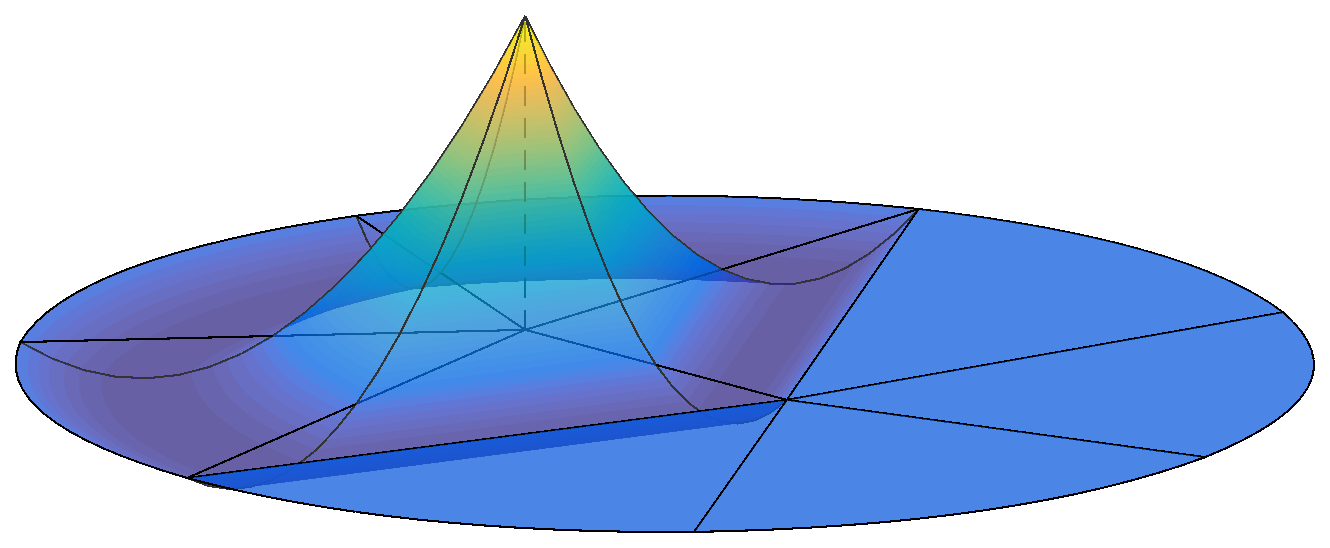
\includegraphics[width=0.48\textwidth]{shape_global_p2_1}
  }
  \subfigure[edge shape function]{
    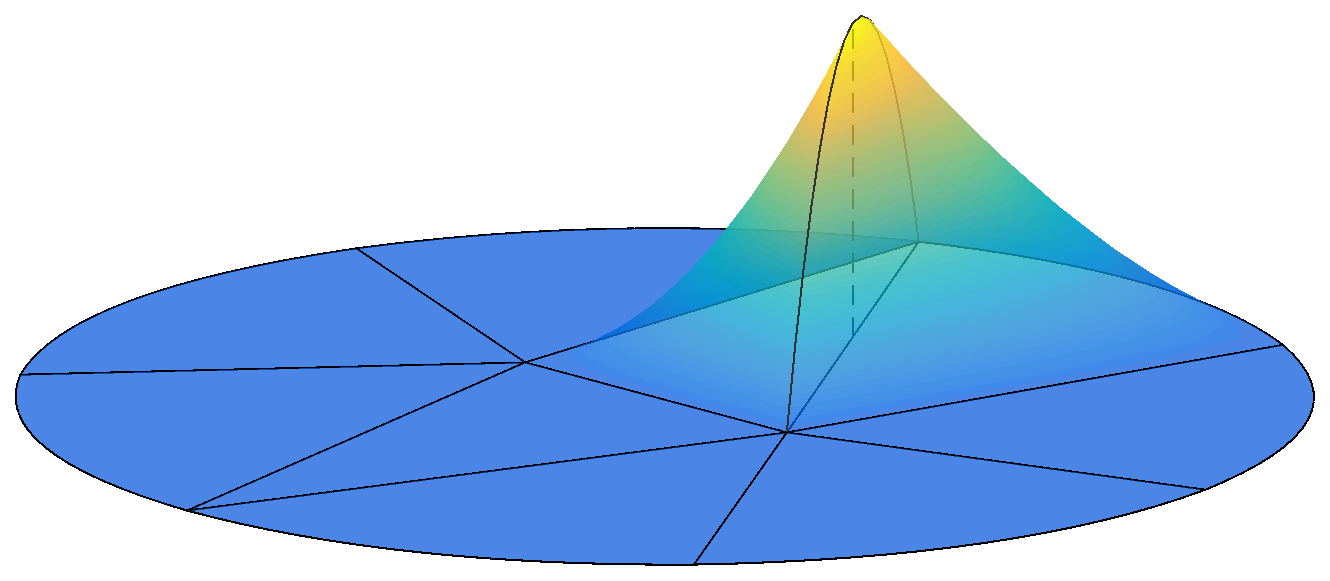
\includegraphics[width=0.48\textwidth]{shape_global_p2_2}
  }
\end{figure}


\begin{figure}
 \centering
 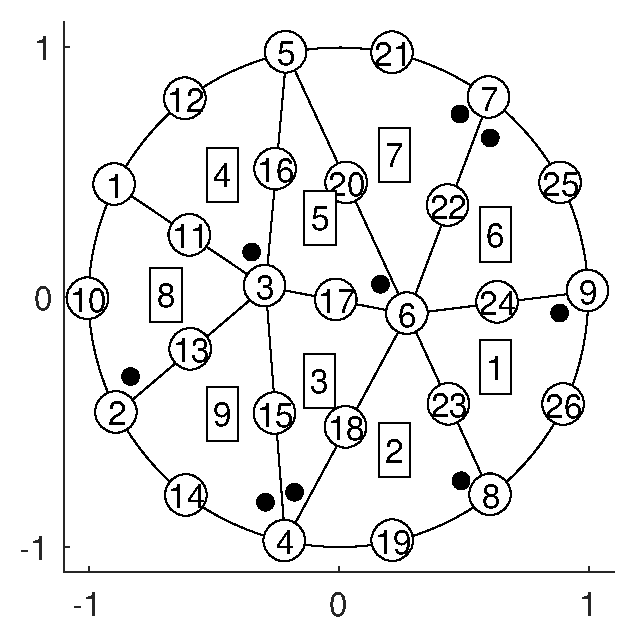
\includegraphics[width=0.4\textwidth]{fe_mesh_p2}
 \caption{$p=2$ mesh.}
 \label{fig:fe_mesh_p2}
\end{figure}
\begin{table}
  \centering
  \subfigure[coordinates]{
    \begin{tabular}{c|cc}
      node & $x_1$ & $x_2$ \\
      \hline
$1$ & $-0.89$ & $\hphantom{-}0.45$ \\ 
$2$ & $-0.89$ & $-0.46$ \\ 
$3$ & $-0.29$ & $\hphantom{-}0.04$ \\ 
$4$ & $-0.21$ & $-0.98$ \\ 
$5$ & $-0.21$ & $\hphantom{-}0.98$ \\ 
$6$ & $\hphantom{-}0.28$ & $-0.07$ \\ 
$7$ & $\hphantom{-}0.60$ & $\hphantom{-}0.80$ \\ 
$8$ & $\hphantom{-}0.61$ & $-0.79$ \\ 
$9$ & $1.00$ & $\hphantom{-}0.02$ \\ 
$10$ & $-1.00$ & $-0.01$ \\ 
$11$ & $-0.59$ & $\hphantom{-}0.25$ \\ 
$12$ & $-0.61$ & $\hphantom{-}0.79$ \\ 
$13$ & $-0.59$ & $-0.21$ \\ 
$14$ & $-0.61$ & $-0.79$ \\ 
$15$ & $-0.25$ & $-0.47$ \\ 
$16$ & $-0.25$ & $\hphantom{-}0.51$ \\ 
$17$ & $-0.01$ & $-0.01$ \\ 
$18$ & $\hphantom{-}0.03$ & $-0.52$ \\ 
$19$ & $\hphantom{-}0.22$ & $-0.98$ \\ 
$20$ & $\hphantom{-}0.03$ & $\hphantom{-}0.46$ \\ 
$21$ & $\hphantom{-}0.22$ & $\hphantom{-}0.98$ \\ 
$22$ & $\hphantom{-}0.44$ & $\hphantom{-}0.36$ \\ 
$23$ & $\hphantom{-}0.44$ & $-0.43$ \\ 
$24$ & $\hphantom{-}0.64$ & $-0.02$ \\ 
$25$ & $\hphantom{-}0.89$ & $\hphantom{-}0.46$ \\ 
$26$ & $\hphantom{-}0.90$ & $-0.43$ \\   
    \end{tabular}
  }
  \subfigure[connectivity]{
    \begin{tabular}{c|cccccc}
      element & node 1 & node 2 & node 3 & node 4 & node 5 & node 6\\
      \hline
$1$ & $9$ & $6$ & $8$ & $23$ & $26$ & $24$ \\ 
$2$ & $8$ & $6$ & $4$ & $18$ & $19$ & $23$ \\ 
$3$ & $4$ & $6$ & $3$ & $17$ & $15$ & $18$ \\ 
$4$ & $3$ & $5$ & $1$ & $12$ & $11$ & $16$ \\ 
$5$ & $6$ & $5$ & $3$ & $16$ & $17$ & $20$ \\ 
$6$ & $7$ & $6$ & $9$ & $24$ & $25$ & $22$ \\ 
$7$ & $7$ & $5$ & $6$ & $20$ & $22$ & $21$ \\ 
$8$ & $2$ & $3$ & $1$ & $11$ & $10$ & $13$ \\ 
$9$ & $4$ & $3$ & $2$ & $13$ & $14$ & $15$ \\ 
    \end{tabular}
  }
  \caption{Node coordinate and connectivity table for $p=2$ mesh shown in Figure~\ref{fig:fe_mesh_p2}}
\end{table}



\section{Interpolation error: linear element in one dimension}
\label{sec:fe_interp_1d}
In this section, we analyze the error associated with the piecewise linear interpolation of functions in one dimension. By way of preliminary, we first provide the definition of \emph{interpolant}.
\begin{definition}[interpolant]
Given $w \in \calV$, an interpolant $\calI_h w$ is an element of $\calV_h$ that satisfies the interpolation condition
\begin{equation*}
  (\calI_h w)(x_i) = w(x_i) \quad i = 1,\dots, N,
\end{equation*}
where $\{x_i \}_{i=1}^N$ is the set of interpolation points.
\end{definition}

We now focus on the piecewise linear space in one dimension.  To this end, given $\Omega \subset \RR$, we introduce an approximation space
\begin{equation*}
  \calV_h = \{ v \in \calV \ | \ v|_K \in \PP^1(K), \ \forall K \in \calT_h \}.
\end{equation*}

\begin{lemma}[One-dimensional linear interpolation error bound for $K$]
  Let $K \equiv [a,b]$ be the domain of length $h \equiv b - a$, $w \in C^2(K)$ be a function we wish to interpolate, and $\calI_h w \in \PP^1(K)$ be the linear interpolant based on the interpolation points $\{a,b\}$. Then, the interpolation error satisfies
  \begin{align}
    \| w - \calI_h w \|_{L^2(K)} &\leq \frac{1}{2} h^{5/2} \| w'' \|_{L^\infty(K)} \label{eq:fe_interp_lin_l2_elem} \\
    | w - \calI_h w |_{H^1(K)} &\leq h^{3/2} \| w '' \|_{L^\infty(K)}. \label{eq:fe_interp_lin_h1_elem}
  \end{align}
  \begin{proof}
    We first introduce an auxiliary function
    \begin{equation*}
      g(s) \equiv (w - \calI_hw)(s) - \left(
      \frac{(w - \calI_h w)(x)}{(x - a)(x-b)}
      \right)(s - a)(s-b).
    \end{equation*}
  We note that $g(x) = g(a) = g(b) = 0$ by construction. Hence $g$ has at least three roots in $K \equiv[a,b]$.  By Rolle's theorem, $g'$ has at least two roots in $K$.  Invoking Rolle's theorem one more time, we conclude that $g''$ has at least one root in $K$; let $\xi \in K$ be one of the roots of $g''$: i.e., $g''(\xi) = 0$.  We now compute the second derivative of $g$:
  \begin{equation*}
    g''(s) = w''(s) - \left(
      \frac{(w - \calI_h w)(x)}{(x - a)(x-b)}
      \right) \cdot 2;
  \end{equation*}
  note that $(\calI_h w)'' = 0$ since $\calI_h w$ is a linear function.  We now evaluate the expression at $\xi$ to obtain
  \begin{equation*}
    0 = w''(\xi) - \left(
      \frac{(w - \calI_h w)(x)}{(x - a)(x-b)}
      \right) \cdot 2, \quad \forall x \in K
  \end{equation*}
  or, equivalently,
  \begin{equation*}
    (w - \calI_h w)(x) = \frac{1}{2} w''(\xi) (x - a)(x - b).
  \end{equation*}
  The $L^2$ error bound follows from
  \begin{align*}
    \| w - \calI_h w \|^2_{L^2(K)}
    &= \int_K (w - \calI_h w)^2 dx
    = \frac{1}{4} \int_K w''(\xi)^2 (x-a)^2 (x-b)^2 dx
    \\
    &\leq\frac{1}{4} \| w'' \|_{L^\infty(K)}^2 \int_K (x-a)^2(x-b)^2 dx
    \leq \frac{1}{4} h^5 \| w'' \|_{L^\infty(K)}^2,
  \end{align*}
  where the inequality follows from $|x-a| < h$ and $|x-b| < h$.  To obtain the $H^1$ error bound, we first note
  \begin{equation*}
    (w - \calI_hw)'(x) = \frac{1}{2} w''(\xi) ((x-a) + (x-b));
  \end{equation*}
  it thus follows
  \begin{align*}
    | w - \calI_h w |^2_{H^1(K)}
    &= \int_K ((w - \calI_h w)')^2 dx
    = \int_K w''(\xi)^2 \frac{1}{4} ((x-a) + (x-b))^2 dx
    \\
    &\leq \| w'' \|_{L^\infty(K)}^2 \int_K \frac{1}{4} ((x-a) + (x-b))^2 dx
    \leq h^3\| w'' \|_{L^2(K)}^2,
  \end{align*}
  where the inequality again follows from $|x - a| < h$ and $|x - b| < h$.
    \end{proof}
\end{lemma}

\begin{proposition}[One-dimensional linear interpolation error bound for $\Omega$]
  Let $\Omega \subset \RR^1$ be the domain, $\calT_h$ be a uniform triangulation over $\Omega$ of characteristic length $h$, $w \in \oplus_{K \in \calT_h}  C^2(K)$ be a function we wish to interpolate, and $\calI_h w \in \calV_h$ be the linear interpolant associated with $\calV_h \equiv \{ v \in C^0(\Omega) \ | \ v|_K \in \PP^1(K), \ \forall K \in \calT_h \}$. Then, the interpolation error satisfies
  \begin{align}
    \| w - \calI_h w \|_{L^2(\Omega)} &\leq \frac{1}{2} h^2 \| w'' \|_{L^\infty(\Omega)} \label{eq:fe_interp_lin_l2} \\
    | w - \calI_h w |_{H^1(\Omega)} &\leq h \| w'' \|_{L^\infty(\Omega)} \label{eq:fe_interp_lin_h1}
  \end{align}
  \begin{proof}
    The $L^2$ error bound follows from the application of~\eqref{eq:fe_interp_lin_l2_elem} to each element:
    \begin{equation*}
      \| w - \calI_h w \|^2_{L^2(\Omega)}
      =
      \sum_{K \in \calT_h} \| w - \calI_h w \|^2_{L^2(K)}
      \leq
      \frac{1}{h} \frac{1}{4} h^5 \| w'' \|_{L^\infty(\Omega)}^2
      = \frac{1}{4} h^4 \| w'' \|_{L^\infty(\Omega)}^2.
    \end{equation*}
    The $H^1$ error bound similarly follows from the application of~\eqref{eq:fe_interp_lin_h1_elem} to each element:
        \begin{equation*}
      \| w - \calI_h w \|^2_{L^2(\Omega)}
      =
      \sum_{K \in \calT_h} \| w - \calI_h w \|^2_{L^2(K)}
      \leq
      \frac{1}{h} h^3 \| w'' \|_{L^\infty(\Omega)}^2
      = h^2 \| w'' \|_{L^\infty(\Omega)}^2.
    \end{equation*}
  \end{proof}
\end{proposition}
The proposition shows that the $L^2$ interpolation error (i) depends on the maximum value of the second derivative $\| w '' \|_{L^\infty(\Omega)}$ and (ii) decreases as $h^2$.  The $H^1$ interpolation error similarly depends on $\| w'' \|_{L^\infty(\Omega)}$ but decreases as $h^1$. 

\section{Interpolation error: general polynomial interpolant}
The interpolation error bound obtained in Section~\ref{sec:fe_interp_1d} can be generalized to (i) higher dimensions, (ii) higher degree polynomials, and (iii) $H^k(\Omega)$ norm for $k \geq 0$.  However, the associated proof, which builds on the Bramble-Hilbert lemma, is beyond the scope of this lecture.  We here simply state the result.
\begin{proposition}
Let $w \in H^s(\Omega)$ be a function we wish to interpolate, $\calT_h$ be a triangulation of a characteristic diameter $h$, $\calI_h w \in \calV_h$ be the piecewise polynomial interpolant of degree $p$ associated with $\calT_h$. Then, the $L^2(\Omega)$ interpolation error satisfies
\begin{align*}
  \| w - \calI_h w \|_{L^2(\Omega)} \leq C h^{r+1} | w |_{H^{r+1}(\Omega)}
\end{align*}
for $r = \min\{ s,p \}$ and some $C$ independent of $h$. Similarly, for $k \geq 0$, the $H^k(\Omega)$ interpolation error satisfies 
\begin{align*}
  \| w - \calI_h w \|_{H^k(\Omega)} \leq C h^{r+1-k} | w |_{H^{r+1}(\Omega)}
\end{align*}
for $r = \min\{ s,p \}$ and some $C$ independent of $h$.
\end{proposition}



%i.e., for a piecewise polynomial space $\calV_h$,
%\begin{equation*}
%  \calV_h \subset \calV \quad \Leftrightarrow \quad \calV_h \subset C^0(\overline \Omega) ,
%\end{equation*}
%where  $C^0(\overline \Omega)$ is the space of continuous functions over $\overline \Omega$.

%Given the continuity requirement, we will construct finite element spaces of the form
%\begin{equation}
%  \calV_h \equiv \{ v \in C^0(\overline \Omega) \ | v |_{K_i} \in \PP^p(K_i), \ i = 1,\dots, n_e \};
%  \label{eq:fe_space}
%\end{equation}
%we recall that $\PP^p(K_i)$ is the space of degree $p$ polynomials over $K_i$.





%% \section{Linear Lagrange element on a line segment}
%% \label{sec:fe_lin_line}
%% We first introduce arguably the simplest finite element: linear Lagrange element on a unit line segment $\tilde K$.  Our unit line segment $\tilde K \equiv (\tilde x^1, \tilde x^2)$ is delineated by two endpoints
%% \begin{equation*}
%%   \tilde x^1 = 0 \quad \text{and} \quad \tilde x^2 = 1.
%% \end{equation*}
%% For the linear polynomial space $\PP^1(\tilde K)$ and the interpolation points $\{\tilde x^1, \tilde x^2\}$, a unique set of \emph{Lagrange basis functions} (or \emph{Lagrange shape functions}) is given by
%% \begin{equation*}
%%   \tilde \phi_1(\tilde x) = 1 - \tilde x \quad \text{and} \quad \tilde \phi_2(\tilde x) = \tilde x.
%% \end{equation*}
%% Note that these basis functions satisfy the interpolation condition
%% \begin{equation*}
%%   \phi_i(\tilde x^j) = \delta_{ij}.
%% \end{equation*}
%% Here $\delta_{ij}$ is the \emph{Kronecker delta}: $\delta_{ij} = 1$ for $i = j$ and $\delta_{ij} = 0$ for $i \neq j$.

%% With these basis functions, we can describe any function $v \in \PP^1(\tilde K)$ as
%% \begin{equation*}
%%   v = \sum_{i=1}^{n_s} \tilde v_i \tilde \phi_i
%% \end{equation*}
%% for $\tilde v_i \equiv v(\tilde x^i)$, $i = 1,2$; the values of the function at the end points are the degree of freedom of the finite element.  Similarly, the derivative of the function is given by
%% \begin{equation*}
%%   \pp{v}{\tilde x} = \sum_{i=1}^{n_s} \tilde v_i \pp{\tilde \phi_i}{\tilde x},
%% \end{equation*}
%% where the direct differentiation of the basis functions yields $\pp{\tilde \phi_1}{\tilde x} = -1$ and $\pp{\tilde \phi_2}{\tilde x} = 1$.


%To see the equivalence, we observe that .  Conversely, if a polynomial space is no
%We hence choose
%\begin{equation*}
%  \calV_h \equiv \{ v \in C^0(\overline \Omega) \ | v |_{K_i} \in \PP^p(K_i), \ i = 1,\dots, n_e \};
%\end{equation*}
%



%% \section{Linear Lagrange finite element on line segments}


%% \label{sec:fe_lin_line}
%% We first introduce arguably the simplest form of finite element: linear Lagrange elements on (one-dimensional) line. In one dimension, any linear function can be expressed as a linear combination of a monomial basis
%% \begin{equation*}
%%   \{ 1, x \};
%% \end{equation*}
%% by construction, $\text{span}\{1,x\} = \PP^1(K)$. Our goal is to find the \emph{Lagrange shape functions}
%% \begin{equation*}
%%   \{ \phi_1, \phi_2 \}
%% \end{equation*}
%% that forms a basis (i.e., $\text{span}\{ \phi_1, \phi_2 \} = \PP^1(K)$) and satisfies the interpolation condition
%% \begin{equation}
%%   \phi_i(x^j) = \delta_{ij};  \label{eq:fe_interp}
%%  % \equiv
%%  % \begin{cases}
%%  %   1, \quad i = j \\
%%  %   0, \quad i \neq j
%%  % \end{cases} 
%% \end{equation}
%% here $\delta_{ij}$ is the \emph{Kronecker delta} such that $\delta_{ij} = 1$ for $i = j$ and $\delta_{ij} = 0$ for $i \neq j$.  To find the basis, we first express the shape functions in terms of the monomial basis:
%% \begin{equation}
%%   \phi_i(x) = a^i_1 + a^i_2 x \quad i = 1, 2.
%%   \label{eq:fe_lin_line_rep}
%% \end{equation}
%% We now apply the interpolation condition~\eqref{eq:fe_interp} to find the coefficients.  For instance, $\phi_1$ must satisfy
%% \begin{equation*}
%%   \bmat{cc}
%%   1 & x^1 \\
%%   1 & x^2 \\
%%   \emat
%%   \bmat{c}
%%   a_1^1 \\ a_2^1 
%%   \emat
%%   =
%%   \bmat{c}
%%   1 \\ 0 
%%   \emat
%% \end{equation*}
%% We can also pose a single matrix equation for the monomial coefficients of all three shape functions: 
%% \begin{equation*}
%%   \bmat{cc}
%%   1 & x^1 \\
%%   1 & x^2 \\
%%   \emat
%%   \bmat{cc}
%%   a_1^1 & a_1^2 \\
%%   a_2^1 & a_2^2 \\
%%   \emat
%%   =
%%   \bmat{cc}
%%   1 & 0 \\
%%   0 & 1 \\
%%   \emat.
%% \end{equation*}
%% We note that the matrix in the first matrix in the left hand side is the \emph{Vandermonde matrix} associated with our monomial basis evaluated at the vertices of the triangle.  The linear equation is well-posed as long as the interpolation points are not colinear, which is equivalent to the condition that the triangle have a finite area.

%% Once we find the coefficients of the shape functions, we can evaluate the value of the functions at any point in the triangle by evaluating~\eqref{eq:fe_lin_line_rep}. We can also differentiate~\eqref{eq:fe_lin_line_rep} to obtain the gradient of the shape functions:
%% \begin{align*}
%%   \pp{\phi_i}{x}(x) = a_2^i
%% \end{align*}
%% The derivatives are constant over the element because the shape functions are linear.

\chapter{Finite element method: error analysis}

\disclaimer

\section{Motivation}
In this lecture, we analyze the error in finite element approximations. As we have seen in the previous lectures, the finite element method seeks a solution to the variational problem in (a family of) finite-dimensional approximation spaces, which often comprise piecewise polynomial functions. As such, the finite element error analysis builds on two distinct ingredients. The first is (quasi-)optimality results which show the ability of the Galerkin method to find a (quasi-)optimal approximation in a given finite-dimensional approximation space.  The second is the approximation theory for the given approximation space; in the case of approximation spaces based on piecewise polynomials, we rely on the polynomial interpolation theory discussed in the previous lecture. The ability to carry out rigorous error analysis is one of the strengths of the finite element method, and we will demonstrate the strength in this lecture.

%In this section and the following sections, we analyze the error in the finite element solution in various norms. By way of preliminaries, we define conditions that are referenced throughout our analysis:
%\begin{assumption}[Assumptions on forms]
%  We make the following assumptions:
%\begin{enumerate}
%  \item $\calV \subset H^1(\Omega)$
%  \item $a(\cdot,\cdot)$ is a bilinear form on $\calV$ (but not necessarily symmetric)
%  \item $a(\cdot,\cdot)$ is $\calV$-continuous with the continuity constant $\gamma$
%  \item $a(\cdot,\cdot)$ is $\calV$-coercive with the coercivity constant $\alpha$
%  \item $\ell(\cdot)$ is a linear form on $\calV$
%  \item $\ell(\cdot)$ is continuous on $\calV$
%\end{enumerate}
%\end{assumption}
\section{Preliminary}
%% By way of preliminaries, we introduce the setting considered throughout this lecture. We first introduce a Lipschitz domain $\Omega \subset \RR^d$.  We next introduce a Hilbert space $\calV$ such that $H^1_0(\Omega) \subset \calV \subset H^1(\Omega)$; the space $\calV$ is endowed with an inner product $(\cdot,\cdot)_\calV$ and the associated induced norm $\| \cdot \|_\calV$. We then introduce a shape-regular family of triangulations $\{\calT_h\}_{h > 0}$ and the associated approximation spaces 
%% \begin{equation}
%%   \calV_h \equiv \{ v \in \calV \ | \ v \circ \calG^K \in \PP^p(\tilde K), \ K \in \calT_h \},
%%   \label{eq:th_fe_Vh}
%% \end{equation}
%% where $\{ \calG^K: \tilde K \to K \}_{K = \calT_h}$ is the geometry mapping associated with the shape-regular triangulations (in the sense of Definitions~\ref{def:th_shape_reg_affine} and \ref{def:th_shape_reg_curved} for polygonal and curved domains, respectively).  We will henceforth refer to the space $\calV_h$ as the $\PP^p$ finite element approximation space (even though the space may contain non-polynomial functions for non-affine meshes).

%% We now introduce a variational problem and the associated finite element approximation.  Throughout this lecture, we assume that the bilinear form $a: \calV \times \calV \to \RR$ is coercive and continuous in $\calV$ and the linear form $\ell: \calV \to \RR$ is continuous in $\calV$.  In addition, \emph{in some cases}, we assume the bilinear form is symmetric; we will clearly state when the symmetry assumption is made.  Our variational problem is as follows: find $u \in \calV$ such that
%% \begin{equation}
%%   a(u,v) = \ell(v) \quad \forall v \in \calV. \label{eq:th_pde}
%% \end{equation}
%% Our finite element problem is as follows: find $u_h \in \calV_h$ such that
%% \begin{equation}
%%   a(u_h,v) = \ell(v) \quad \forall v \in \calV_h.
%% \end{equation}
%% We will henceforth refer to the solution to~\eqref{eq:th_fe}, associated with the approximation space $\calV_h$ defined in~\ref{eq:th_fe_Vh}, as the $\PP^p$ finite element approximation.  Because the bilinear form is coercive and continuous and the linear form is continuous, the solutions to \ref{eq:th_pde} and \ref{eq:th_fe} exist and are unique by the Lax-Milgram theorem, Theorem~\ref{thm:lax_milgram}.  For convenience, we group our common assumptions in the following.

By way of preliminaries, we introduce a set of assumptions used throughout this lecture.  The first is a set of assumptions on the (abstract) variational problem.
\begin{assumption}
  \label{ass:th_fe_form}
  We consider the following.
  \begin{enumerate}
  \item The domain $\Omega \subset \RR^d$ has a Lipschitz boundary.
  \item The Hilbert space $\calV$ satisfies $H^1_0(\Omega) \subset \calV \subset H^1(\Omega)$. The space $\calV$ is endowed with an inner product $(\cdot,\cdot)_\calV$ and the associated induced norm $\| \cdot \|_\calV$, which is equivalent to $\| \cdot \|_{H^1(\Omega)}$.
  \item The bilinear form $a: \calV \times \calV \to \RR$ is coercive and continuous in $\calV$ with the coercivity and continuity constants $\alpha > 0$ and $\gamma < \infty$, respectively; i.e., $a(v,v) \geq \alpha \| v \|_\calV^2$ $\forall v \in \calV$, and $|a(w,v)| \leq \gamma \| w\|_\calV \| v \|_\calV$ $\forall w,v \in \calV$.
  \item The linear form $\ell: \calV \to \RR$ is continuous in $\calV$; i.e., $\exists c < \infty$ such that $|\ell(v)| \leq c \| v \|_\calV$ $\forall v \in \calV$.
  \end{enumerate}
\end{assumption}
Assumption~\ref{ass:th_fe_form} does not assume the bilinear form is symmetric; we will clearly state the symmetry assumption whenever it is required as an additional assumption.  We also note that Assumption~\ref{ass:th_fe_form} is a set of assumptions of the Lax-Milgram theorem, Theorem~\ref{thm:lax_milgram}.

We next introduce the assumptions that define the variational solution and the associated finite element approximation.
\begin{assumption}
  \label{ass:th_fe_soln}
  We consider the following.
  \begin{enumerate}
  \item The solution $u \in \calV$ satisfies
    \begin{equation}
      \label{eq:th_pde}
      a(u,v) = \ell(v) \quad \forall v \in \calV.
    \end{equation}
  \item The finite element approximation $u_h \in \calV_h$ satisfies
    \begin{equation}
      \label{eq:th_fe}
      a(u_h,v) = \ell(v) \quad \forall v \in \calV_h
    \end{equation}
    for some finite-dimensional subspace $\calV_h \subset \calV$.
  \end{enumerate}
\end{assumption}
Assumption~\ref{ass:th_fe_soln} does not specify the finite element approximation space $\calV_h$ other than that it is a subspace of $\calV$; in particular, we do not assume the space $\calV_h$ is a space of piecewise polynomials.  Given Assumption~\ref{ass:th_fe_form}, both the variational problem~\eqref{eq:th_pde} and finite element problem~\eqref{eq:th_fe} are well posed thanks to the Lax-Milgram theorem.

We finally introduce a particular family of piecewise polynomial approximation spaces.
\begin{assumption}
  \label{ass:th_fe_Vh}
  We consider the following:
  \begin{enumerate}
  \item The family of triangulations $\{ \calT_h \}$ is shape-regular in the in the sense of Definitions~\ref{def:th_shape_reg_affine} and \ref{def:th_shape_reg_curved} for polygonal and curved domains, respectively.
  \item The approximation spaces are given by 
  \begin{equation}
    \calV_h \equiv \{ v \in \calV \ | \ v \circ \calG^K \in \PP^p(\tilde K), \ K \in \calT_h \},
    \label{eq:th_fe_Vh}
  \end{equation}
  where $\{ \calG^K: \tilde K \to K \}_{K = \calT_h}$ is the geometry mapping associated with the shape-regular triangulations.
  \end{enumerate}
  \end{assumption}
  Note that~\eqref{eq:th_fe_Vh} is one particular example of an approximation space for the finite element approximation~\eqref{eq:th_fe}.  We will henceforth refer to the space $\calV_h$ in \eqref{eq:th_fe_Vh} as the $\PP^p$ finite element approximation space (even though the space may contain non-polynomial functions for isoparametric approximation of curved-domains). In addition, we will refer to the solution $u_h \in \calV_h$ to \eqref{eq:th_fe} associated with $\calV_h$ in \eqref{eq:th_fe_Vh} as the $\PP^p$ finite element approximation.  

\section{Galerkin orthogonality}
We now introduce \emph{Galerkin orthogonality}, a relationship that will be used throughout our analysis of error in finite element approximations.
\begin{lemma}[Galerkin orthogonality]
  Suppose Assumptions~\ref{ass:th_fe_form} and \ref{ass:th_fe_soln} hold. The error $u - u_h \in \calV$ satisfies 
  \begin{equation*}
    a(u - u_h, v) = 0 \quad \forall v \in \calV_h.
  \end{equation*}
  \begin{proof}
    The condition~\eqref{eq:th_pde} implies $a(u,v) = \ell(v)$, $\forall v \in \calV_h \subset \calV$.  The subtraction of \eqref{eq:th_fe} from the relationship yields
    \begin{equation*}
      a(u - u_h, v) = a(u,v) - a(u_h,v) = \ell(v) - \ell(v) = 0 \quad \forall v \in \calV_h,
    \end{equation*}
    which is the desired relationship.
  \end{proof}
\end{lemma}

\section{Error bounds in energy norm}
In this section we consider a symmetric, coercive bilinear form and assess our error in \emph{energy norm}.
\begin{definition}[energy norm]
  Given a symmetric, coercive, and continuous bilinear form $a: \calV \times \calV \to \RR$, the energy norm $\| \cdot \|_a : \calV \to \RR_{\geq 0}$ is defined by
  \begin{equation*}
    \| v \|_a \equiv \sqrt{a(v,v)} \quad \forall v \in \calV.
  \end{equation*}
\end{definition}
Because the bilinear form is symmetric and coercive, the bilinear form $a(\cdot,\cdot)$ is in fact an inner product that satisfies the requirements on (i) the linearity, (ii) symmetry, and (iii) Cauchy-Shwarz inequality.  The energy norm is the induced norm associated with this inner product; the norm hence satisfies the requirements on (i) the linearity, (ii) positivity, and (iii) triangle inequality.

The energy norm is \emph{equivalent} to $\| \cdot \|_{H^1(\Omega)}$ in the following sense.
\begin{definition}[equivalence of norms]
  Given a Hilbert space $\calV$, a norm $\| \cdot \|_A$ is said to be equivalent to a norm $\| \cdot \|_B$ if there exist $c > 0$ and $C < \infty$ such that
  \begin{equation*}
    c \| v \|_{B} \leq \| v \|_A \leq C \| v \|_{B} \quad \forall v \in \calV.
  \end{equation*}
\end{definition}
\begin{lemma}[equivalence of energy and $H^1$ norm]
  Suppose Assumption~\ref{ass:th_fe_form} holds for a symmetric bilinear form.  The energy norm $\| \cdot \|_a$ is equivalent to the $H^1$ norm $\| \cdot \|_{H^1(\Omega)}$.
  \begin{proof}
    From coercivity and continuity of $a(\cdot,\cdot)$ in $\calV$, we immediately obtain
    \begin{equation*}
      \alpha \| v \|_\calV^2 \leq a(v,v) \equiv \| v \|_a^2 \leq \gamma \| v \|_\calV^2 \quad \forall v \in \calV,
    \end{equation*}
    where $\alpha > 0$ and $\gamma < \infty$ are the coercivity and continuity constants, respectively. %Taking the square root of the inequality yields the desired relationship.
  \end{proof}
\end{lemma}

We now show that the finite element approximation is optimal in the energy norm.
\begin{proposition}[energy-norm error bound]
  \label{prop:th_energy_bound}
  Suppose Assumptions~\ref{ass:th_fe_form} and \ref{ass:th_fe_soln} hold for a symmetric bilinear form.   The finite element approximation is optimal in the energy norm in the sense that
  \begin{equation}
    \| u - u_h \|_a = \inf_{w_h \in \calV_h} \| u - w_h \|_a.
    \label{eq:th_energy_bound}
  \end{equation}
  \begin{proof}
    Let $w_h$ be an arbitrary element in $\calV_h$ and express it as $w_h = u_h + v_h$ for $v_h \in \calV_h$.  Then,
\begin{align*}
  \| u - w_h \|_a^2 &= \| u - u_h - v_h \|_a^2
  = a(u - u_h - v_h, u - u_h - v_h) \\
  &= a(u - u_h, u - u_h) - 2 \underbrace{ a(u - u_h, v_h) }_{= 0 \text{ by Galerkin orthogonality}} + \underbrace{ a(v_h,v_h) }_{> 0 \text{ for $v_h \neq 0$ by coercivity}}
  \\
  &> \| u - u_h \|_a^2 \quad \forall v_h \neq 0, % \quad \text{ or, equivalently, $\forall w_h \neq u_h$}.
\end{align*}
or, equivalently, $\forall w_h \neq u_h$.
  \end{proof}
\end{proposition}
The optimality of the finite element error in the energy norm implies the following: even \emph{if} we knew the exact solution $u \in \calV$ to~\eqref{eq:th_pde}, we could not find a $w_h \in \calV_h$ that is more accurate in the energy norm than $u_h \in \calV_h$. This optimality result is a direct consequence of Galerkin orthogonality, which states that the error $u - u_h \in \calV$ is orthogonal to the space $\calV_h$ in the inner product associated with the bilinear form $a: \calV \times \calV \to \RR$. In other words, $u_h \in \calV_h$ is the $a$-orthogonal projection of $u \in \calV$ onto $\calV_h \subset \calV$.

We may obtain a particular $h$-convergence result for $\PP^p$ finite element approximations.
\begin{proposition}[energy-norm error bound: $h$ convergence]
  \label{prop:th_energy_bound_poly}
  Suppose Assumptions~\ref{ass:th_fe_form}, \ref{ass:th_fe_soln}, and \ref{ass:th_fe_Vh} hold for a symmetric bilinear form. If $u \in H^1(\Omega) \cap H^{s+1}(\calT_h)$, then
  \begin{equation*}
    \| u - u_h \|_a \leq C h^r | u |_{H^{r+1}(\calT_h)}
  \end{equation*}
  for $r \equiv \min\{s,p\}$ and some constant $C < \infty$ independent of $u$ and $h$.  (Here, $H^k(\calT_h)$ and $| \cdot |_{H^{k}(\calT_h)}$ are the broken space and semi-norm, respectively, in Definition~\ref{def:th_broken_Hk}.)
  \begin{proof}
    The bound follows from the energy-norm error bound in Proposition~\eqref{prop:th_energy_bound} and the polynomial interpolation error bound in Proposition~\ref{prop:th_interp_gen}:
    \begin{align*}
      \| u - u_h \|_a &= \inf_{w_h \in \calV_h} \| u - w_h \|_a
      & \text{(energy-norm error bound)}  \\
      &\leq \| u - \calI_h u \|_a &\text{($w_h = \calI_h u$)} \\
      &\leq \gamma \| u - \calI_h u \|_{H^1(\Omega)} &\text{(continuity of $a(\cdot,\cdot)$)} \\
      &\leq \gamma C_\calI h^r | u |_{H^{r+1}(\calT_h)}. &\text{(interpolation error bound)}
    \end{align*}
    We set $C \equiv \gamma C_\calI$ to obtain the desired relationship.
  \end{proof}
\end{proposition}

We observe that, if the solution $u$ is smooth in the sense $u \in H^1(\Omega) \cap H^{p+1}(\calT_h)$, then the error in the $\PP^p$ finite element approximation converges as $h^p$ in the energy norm.  If the solution is not smooth in the sense $u \notin H^1(\Omega) \cap H^{p+1}(\calT_h)$, then the convergence rate of the finite element approximation is limited by the regularity of the solution.  We however note that the regularity of the solution is assessed in the broken norm $| u |_{H^{s+1}(\calT_h)}$; if the irregular features in the solution, such as kinks, align with the triangulation, then the features may not deteriorate the convergence rate.  Hence, for problems with known irregular features resulting from, say, discontinuous source functions or discontinuous diffusivity field, it is important to align the triangulation with the features.

\section{Error bounds in $\calV$ and $H^1(\Omega)$ norms}
In this section, we obtain error bounds in the $\calV$ and $H^1(\Omega)$ norms.  As in Assumption~\ref{ass:th_fe_form}, we assume $H^1_0(\Omega) \subset \calV \subset H^1(\Omega)$ so that $\| \cdot \|_\calV$ is equivalent to $\| \cdot \|_{H^1(\Omega)}$.  The first bound is for a variational problem with a symmetric, coercive bilinear form.
\begin{lemma}[C\'ea's lemma (symmetric)]
  \label{lemma:th_cea_sym}
   Suppose Assumptions~\ref{ass:th_fe_form} and \ref{ass:th_fe_soln} hold for a symmetric bilinear form. Then, 
  \begin{equation}
    \| u - u_h \|_\calV \leq \sqrt{\frac{\gamma}{\alpha}} \inf_{w_h \in \calV_h} \| u - w_h \|_\calV.
    \label{eq:th_cea_sym}
  \end{equation}
%  for the coercivity constant $\alpha$ and the continuity constant $\gamma$
  \begin{proof}
    The bound follows from the coercivity and continuity of the bilinear form and the energy-norm error bound in Proposition~\eqref{prop:th_energy_bound}:
    \begin{align*}
      \alpha \| u - u_h \|^2_\calV
      &\leq a(u - u_h, u - u_h) & \text{(coercivity)} \\
      &\leq \| u - u_h \|_a^2 & \text{(energy norm)} \\
      & = \inf_{w_h \in \calV_h} \| u - u_h \|_a^2 & \text{(energy-norm error bound)} \\
      & = \gamma \| u - u_h \|^2_\calV & \text{(continuity)}.
    \end{align*}
    The division by $\alpha > 0$ yields the desired inequality.
  \end{proof}
\end{lemma}

The second bound is for a variational problem with a bilinear form that is coercive but not necessarily symmetric.
\begin{lemma}[C\'ea's lemma (nonsymmetric)]
  \label{lemma:th_cea_nonsym}
   Suppose Assumptions~\ref{ass:th_fe_form} and \ref{ass:th_fe_soln} hold. Then, 
  \begin{equation}
    \| u - u_h \|_\calV \leq \frac{\gamma}{\alpha} \inf_{w_h \in \calV_h} \| u - w_h \|_\calV.
    \label{eq:th_cea}
  \end{equation}
%  for the coercivity constant $\alpha$ and the continuity constant $\gamma$.
  \begin{proof}
    The result is trivial for $\| u - u_h \|_\calV = 0$.  For $\| u - u_h \|_\calV \neq 0$, we observe
    \begin{align*}
      \alpha \| u - u_h \|^2_\calV
      &\leq a(u - u_h, u - u_h) & \text{(coercivity)} \\
      &= a(u - u_h, u - w_h) + a(u - u_h, w_h - u_h) &\text{(bilinearity)} \\
      &= a(u - u_h, u - w_h) &\text{(Galerkin orthogonality)} \\
      &\leq \gamma \| u - u_h \|_\calV \| u - w_h \|_\calV &\text{(continuity)}.
    \end{align*}
    The division by $\alpha \| u - u_h \|_\calV > 0$ yields the desired result.
  \end{proof}
\end{lemma}
Because $\gamma/\alpha \geq 1$ by the definition of the continuity and coercivity constants, the bound~\eqref{eq:th_cea} for nonsymmetric bilinear forms, which applies to more general problems, is looser than the bound~\eqref{eq:th_cea_sym} for symmetric bilinear forms.  In both cases, we observe that the finite element approximation is quasi-optimal in the sense that $\| u - u_h \|_\calV$ is at most a constant multiple of the best-fit error $\inf_{w_h \in \calV_h} \| u - w_h \|_\calV$, where the constant is independent of the approximation space $\calV_h$.

Given the quasi-optimality results of C\'ea's lemma, we can readily obtain particular $h$-convergence results for $\PP^p$ finite element approximations.
\begin{proposition}[$\calV$-norm error bound: $h$ convergence]
  \label{prop:th_fe_vnorm_hconv}
   Suppose Assumptions~\ref{ass:th_fe_form}, \ref{ass:th_fe_soln}, and \ref{ass:th_fe_Vh} hold. If $u \in H^1(\Omega) \cap H^{s+1}(\calT_h)$, then
  \begin{equation}
    \| u - u_h \|_\calV \leq C h^{r} | u |_{H^{r+1}(\calT_h)}
  \end{equation}
  for $r \equiv \min\{ s,p \}$ and some $C < \infty$ independent of $u$ and $h$.
  \begin{proof}
    We invoke C\'ea's lemma~\ref{lemma:th_cea_sym}, the equivalence of $\| \cdot \|_{\calV}$ and $\| \cdot \|_{H^1(\Omega)}$, and the polynomial interpolation error bound in Proposition~\ref{prop:th_interp_gen}.
  \end{proof}
\end{proposition}
\begin{proposition}[$H^1(\Omega)$-norm $h$ convergence]
  Suppose Assumptions~\ref{ass:th_fe_form}, \ref{ass:th_fe_soln}, and \ref{ass:th_fe_Vh} hold. If $u \in H^1(\Omega) \cap H^{s+1}(\calT_h)$, then
  \begin{equation}
    \| u - u_h \|_{H^1(\Omega)} \leq C h^{r} | u |_{H^{r+1}(\calT_h)}
  \end{equation}
  for $r \equiv \min\{ s,p \}$ and some $C < \infty$ independent of $u$ and $h$.
  \begin{proof}
    The result follows from Proposition~\ref{prop:th_fe_vnorm_hconv} and the equivalence of $\| \cdot \|_{\calV}$ and $\| \cdot \|_{H^1(\Omega)}$.
  \end{proof}
\end{proposition}

Similar to the energy norm of the error, we observe that, if the solution $u$ is smooth in the sense $u \in H^1(\Omega) \cap H^{p+1}(\calT_h)$, then the error in $\PP^p$ finite element approximations converges as $h^p$ in the $\calV$ or $H^1(\Omega)$ norm.  If the solution is not smooth, then the convergence rate of the finite element approximations is limited by the regularity of the solution. 


\section{Error bounds in $L^2(\Omega)$ norm}
We now analyze the convergence of finite element approximations in $L^2(\Omega)$ norm.  Unfortunately, the $L^2(\Omega)$ error analysis relies on an equation-specific result called the \emph{elliptic regularity estimate}.  Hence, in this section, unlike in the previous sections, we restrict ourselves to (variable coefficients) advection-reaction-diffusion equation.  (The regularity estimate holds also for other equations, but we here state a concrete result for the specific equation.)

\begin{lemma}[elliptic regularity estimate]
  \label{lemma:th_elliptic_reg}
  Let $\Omega \subset \RR^d$ be a Lipschitz domain, $\calV$ be a Hilbert space such that $H_0^1(\Omega) \subset \calV \subset H^1(\Omega)$, and let $a: \calV \times \calV \to \RR$ be
  \begin{equation*}
    a(w,v) = \int_\Omega (\nabla v \cdot a \nabla w + v b \cdot \nabla w + c v w) dx,  \quad \forall w, v \in \calV,
  \end{equation*}
  for $a \in C^{1}(\bar \Omega)^{d \times d}$ and elliptic, $b \in C^0(\bar \Omega)^d$, $c \in C^0(\bar \Omega)$.  Consider the following weak problem: find $u \in \calV$ such that
  \begin{equation*}
    a(u,v) = (f,v)_{L^2(\Omega)} \quad \forall v \in \calV,
  \end{equation*}
  where $f \in L^2(\Omega)$. Then the solution $u$ satisfies
  \begin{equation*}
    \| u \|_{H^2(\Omega)} \leq C_{\rm reg} \| f \|_{L^2(\Omega)}
  \end{equation*}
  for some $C_{\rm reg} < \infty$.
  \begin{proof}
    Proof is beyond the scope of this course.  See, e.g., Ern and Guermond (2004). %, \emph{Theory and practice of finite element method}, Theorem 3.10.
  \end{proof}
\end{lemma}
\begin{proposition}[$L^2$-norm error bound (Aubin-Nitsche)]
  \label{prop:th_aubin_nitsche}
  Suppose Assumptions~\ref{ass:th_fe_form}, \ref{ass:th_fe_soln}, and \ref{ass:th_fe_Vh} as well as the conditions of the elliptic regularity estimate, Lemma~\ref{lemma:th_elliptic_reg}, hold. Then, 
  \begin{equation*}
    \| u - u_h \|_{L^2(\Omega)} \leq C h \| u-u_h \|_\calV,
  \end{equation*}
  for some $C < \infty$ independent of $u$ and $h$.
  \begin{proof}
    The proof is by so-called \emph{Aubin-Nitsche trick}. We first pose a dual problem: find $\psi \in \calV$ such that
    \begin{equation*}
      a(w,\psi) = (w,e)_{L^2(\Omega)} \quad \forall w \in \calV
    \end{equation*}
    for $e \equiv u - u_h$. We then observe that
    \begin{equation*}
      \| e \|_{L^2(\Omega)}^2 = a(e, \psi)
      = a(e, \psi - \Pi_{H^1(\Omega)} \psi)
      \leq \gamma \| e \|_\calV \| \psi - \calI_h \psi \|_\calV.
    \end{equation*}
    We note that, since $u \in H^1(\Omega)$ and $u_h \in H^1(\Omega)$,  $e \equiv u - u_h \in \calV \subset H^1(\Omega) \subset L^2(\Omega)$; by the elliptic regularity estimate, $\| \psi \|_{H^2(\Omega)} \leq C_{\rm reg} \| e \|_{L^2(\Omega)}$. We hence obtain
    \begin{align*}
      \| \psi - \calI_h \psi \|_\calV
      &=\| \psi - \calI_h \psi \|_{H^1(\Omega)} & \text{(definition of $\calV$ norm)} \\
      &\leq C_\calI h \| \psi \|_{H^2(\Omega)} & \text{(interpolation error bound)}\\
      &\leq C_\calI C_{\rm reg} h  \| e \|_{L^2(\Omega)}. & \text{(elliptic regularity estimate)}
    \end{align*}
    It follows
    \begin{equation*}
      \| e \|_{L^2(\Omega)}^2 \leq \gamma C_\calI C_{\rm reg} h \| e \|_{L^2(\Omega)} \| e \|_\calV .
    \end{equation*}
    The division by $\| e \|_{L^2(\Omega)}$ yields the desired bound.
  \end{proof}
\end{proposition}

\begin{proposition}[$L^2(\Omega)$-norm error bound: $h$ convergence]
  Suppose Assumptions~\ref{ass:th_fe_form}, \ref{ass:th_fe_soln}, and \ref{ass:th_fe_Vh} as well as the conditions of the elliptic regularity estimate, Lemma~\ref{lemma:th_elliptic_reg}, hold. If $u \in H^1(\Omega) \cap H^{s+1}(\calT_h)$, then
  \begin{equation*}
    \| u - u_h \|_{L^2(\Omega)} \leq C h^{r+1} | u |_{H^{r+1}(\calT_h)}
  \end{equation*}
  for $r \equiv \min\{ s,p\}$ and some $C < \infty$ independent of $u$ and $h$.
  \begin{proof}
    The result is a direct consequence of Propositions~\ref{prop:th_aubin_nitsche} and \ref{prop:th_fe_vnorm_hconv}:
    \begin{align*}
      \| u - u_h \|_{L^2(\Omega)}
      &\leq C h \| u-u_h \|_\calV & \text{(Aubin-Nitsche)} \\
      &\leq C' h^{r+1} | u |_{H^{r+1}(\calT_h)} . &\text{($h$ convergence in $\| \cdot \|_\calV$)} 
    \end{align*}
  \end{proof}
\end{proposition}
The proposition shows that, if the solution is smooth in the sense $u \in H^1(\Omega) \cap H^{p+1}(\calT_h)$, then the $L^2(\Omega)$ norm of the error converges as $h^{p+1}$ --- the rate one higher than the $H^1(\Omega)$ or $\calV$ norm of the error.  In particular, we note that the $L^2(\Omega)$ norm of the error in the linear ($\PP^1$) finite element approximations converge as $h^2$; because the $L^2(\Omega)$ norm is arguably the most popular metric for the assessment of the error in engineering, the linear finite element method is often quoted as a second-order method in the field.

\section{Error bounds for functional outputs}
In this section we consider the error in an \emph{output} or \emph{quantity of interest}. To begin, we introduce a linear functional associated with the output,
\begin{equation*}
  \ell^o : \calV \to \RR;
\end{equation*}
we assume that the functional is continuous in $\calV$: $\exists c < \infty$ such that $| \ell^o(w) | \leq c \| w \|_\calV$ $\forall w \in \calV$.

In order to characterize output error, we first introduce the \emph{dual problem}: find $\psi \in \calV$ such that
\begin{equation}
  \label{eq:th_dual}
  a(w,\psi) = \ell^o(w) \quad \forall w \in \calV.
\end{equation}
The well-posedness of the dual problem follows from the Lax-Milgram theorem, Theorem~\ref{thm:lax_milgram}, for a $\calV$-coercive, $\calV$-continuous (but not necessarily symmetric) bilinear form $a(\cdot,\cdot)$, and $\calV$-continuous linear form $\ell^o(\cdot)$.  The solution $\psi \in \calV$ is called the \emph{dual solution} or \emph{adjoint}.  (To contrast, the variational problem~\eqref{eq:th_pde} is sometimes called the \emph{primal problem} and the solution $u$ is called the \emph{primal solution}.)

\begin{proposition}[output error bound (symmetric)]
  \label{prop:th_output_sym}
  Suppose Assumptions~\eqref{ass:th_fe_form} and \eqref{ass:th_fe_soln} hold for a symmetric bilinear form. Let $\ell^o: \calV \to \RR$ be a continuous linear functional. Then,
\begin{equation*}
  |\ell^o(u) - \ell^o(u_h)| \leq
  \inf_{w_h \in \calV_h} \| u - w_h \|_a \inf_{v_h \in \calV_h} \| \psi - v_h \|_a,
\end{equation*}
where $\psi$ is the solution to the dual problem~\ref{eq:th_dual}.
\begin{proof}
  We observe that, $\forall v_h \in \calV_h$, 
\begin{align*}
  |\ell^o(u) - \ell^o(u_h)|
  &= |\ell^o(u - u_h)| & \text{(linearity of $\ell^o$)} \\
  &= |a(u-u_h,\psi)| & \text{(definition of adjoint $\psi$)} \\
  &= |a(u-u_h,\psi-v_h)| & \text{(Galerkin orthogonality)} \\
  &\leq \| u - u_h \|_a \| \psi - v_h \|_a & \text{(Cauchy-Schwarz)} \\
  &\leq \inf_{w_h \in \calV_h} \| u - w_h \|_a \| \psi - v_h \|_a. & \text{(energy-error optimality of $u_h$)}
\end{align*}
We then take $v_h \in \calV_h$ to be the minimizer of $\| \psi - v_h \|_a$ to obtain the desired result.
\end{proof}
\end{proposition}

\begin{proposition}[output error bound (nonsymmetric)]
  \label{prop:th_output_nonsym}
   Suppose Assumptions~\eqref{ass:th_fe_form} and \eqref{ass:th_fe_soln} hold. Let $\ell^o: \calV \to \RR$ be a continuous linear functional.  Then,
\begin{equation*}
  |\ell^o(u) - \ell^o(u_h)|
  \leq \frac{\gamma^2}{\alpha} \inf_{w_h \in \calV_h} \| u - w_h \|_\calV \inf_{v_h \in \calV_h} \| \psi - v_h \|_\calV,
\end{equation*}
where $\psi$ is the solution to the dual problem~\ref{eq:th_dual}.
\begin{proof}
  We observe that, $\forall v_h \in \calV_h$, 
  \begin{align*}
    |\ell^o(u) - \ell^o(u_h)|
    &= |\ell^o(u - u_h)| & \text{(linearity of $\ell^o$)} \\
    &= |a(u-u_h,\psi)| & \text{(definition of adjoint $\psi$)} \\
    &= |a(u-u_h,\psi-v_h)| & \text{(Galerkin orthogonality)} \\
    &\leq \gamma \| u - u_h \|_\calV \| \psi - v_h \|_\calV & \text{(continuity of $a(\cdot,\cdot)$)} \\
    &\leq \frac{\gamma^2}{\alpha} \inf_{w_h \in \calV_h} \| u - w_h \|_\calV \| \psi - v_h \|_\calV. & \text{($\| \cdot \|_\calV$ error bound of $u_h$)}
  \end{align*}
  We then take $v_h \in \calV_h$ to be the minimizer of $\| \psi - v_h \|_a$ to obtain the desired result.
\end{proof}
\end{proposition}

\begin{proposition}[output error bound: $h$ convergence]
   Suppose Assumptions~\ref{ass:th_fe_form}, \ref{ass:th_fe_soln}, and \ref{ass:th_fe_Vh} hold. Let $\ell^o: \calV \to \RR$ be a continuous linear functional.  If $u \in H^1(\Omega) \cap H^{s+1}(\calT_h)$ and $\psi \in H^1(\Omega) \cap H^{s'+1}(\calT_h)$ for $\psi$ the solution to the dual problem~\ref{eq:th_dual}, then
  \begin{equation*}
    | \ell^o(u) - \ell^o(u_h) | \leq C h^{r + r'} | u |_{H^{r+1}(\calT_h)} | \psi |_{H^{r'+1}(\calT_h)}
  \end{equation*}
  for $r \equiv \min\{ s,p \}$, $r' \equiv \min\{ s',p \}$, and some constant $C < \infty$ independent of $u$, $\psi$, and $h$.
  \begin{proof}
    The result follows from (i) Proposition~\ref{prop:th_output_nonsym},  (ii) the equivalence of $\|\cdot\|_\calV$ and $\| \cdot \|_{H^1(\Omega)}$, and (iii) the polynomial interpolation error bound in Proposition~\ref{prop:th_interp_gen}.
  \end{proof}
\end{proposition}
The proposition shows that for a smooth solution $u \in H^1(\Omega) \cap H^{p+1}(\calT_h)$ \emph{and} adjoint $\psi \in H^1(\Omega) \cap H^{p+1}(\calT_h)$, the output converges as $h^{2p}$. The convergence rate for the output error is \emph{twice} that for the $\calV$ or $H^1(\Omega)$ norm of the error.  This result is often referred to as \emph{output superconvergence}.  (The output superconverges because the finite element approximation is by construction \emph{dual consistent}: the dual of the discrete problem is the discretization of the continuous dual problem.  Not all discretizations for boundary value problems have this property.)


\section{Generalization: other approximation spaces}
Throughout this lecture, we presented two types of error bounds. First, under Assumptions~\ref{ass:th_fe_form} and \ref{ass:th_fe_soln}, we obtained the (quasi-)optimality results that show the Galerkin finite element method achieves errors that are only some fixed constant away from the best-fit solution in a given approximation space (e.g., C\'ea's lemma, Lemma~\ref{lemma:th_cea_nonsym}).  Second, under Assumptions~\ref{ass:th_fe_form}, \ref{ass:th_fe_soln}, and \ref{ass:th_fe_Vh}, we obtained the particular $h$-convergence results for $\PP^p$ finite element approximation spaces. The results of the first type, such as C\'ea's lemma
\begin{equation*}
  \| u - u_n \|_{\calV} \leq \frac{\gamma}{\alpha} \inf_{w_n \in \calV_n} \| u - w_n \|_{\calV},
\end{equation*}
applies to any (family of) finite-dimensional approximation spaces $\{ \calV_n \}_{n > 1}$.  The Galerkin finite element method will find a quasi-optimal approximations $\{u_n\}_{n > 1}$ in any family of approximation spaces $\{\calV_n \}_{n > 1}$. %; given an approximation space $\calV_n$ in which the solution $u$ can be well-approximated, the Galerkin finite element method will find a good member of $\calV_n$ that well approximates $u$.  

We can derive various methods based on the Galerkin projection by choosing different approximation spaces. The ``standard'' finite element method based on $h$ refinement considers $\{ \calV_h \}_{h > 0}$ defined by Assumption~\ref{ass:th_fe_Vh}; if the exact solution is in $H^1(\Omega) \cap H^{p+1}(\calT_h)$, the $\calV$-norm of the error converges as $h^p$. The spectral method considers approximation spaces consist of high-order global polynomials, $\calV_p \equiv \{ v \in \calV \ | \ v \in \PP^p(\Omega) \}$; if the exact solution is analytic, then the $\calV$-norm of the error converges as $\exp(-Cp)$ for some $C$ independent of $p$, achieving the so-called \emph{exponential convergence}. The $hp$ adaptive finite element method constructs a sequence of piecewise polynomial spaces of varying $h$ and $p$ tailored for the specific solution we wish to approximate. The extended finite element method (XEFM) or generalized finite element method (GFEM) considers a family of approximation spaces comprise specialized (non-polynomial) functions tailored for the specific features (e.g., corner singularity).  The reduced-basis method, a model reduction method for parametrized PDEs, considers approximation spaces comprise specialized (non-polynomial) functions tailored for the parametric manifold.  All of these techniques rely on the Galerkin projection, which identifies a quasi-optimal approximation in a given approximation space.

\section{Summary}
We summarize key points of this lecture:
\begin{enumerate}
%\item The Galerkin orthogonality, $a(e,v) = 0$ $\forall v \in \calV_h$, is a key ingredient of finite element error analysis.
\item For a symmetric, coercive problem, the energy norm is given by $\| \cdot \|_a \equiv \sqrt{a(\cdot,\cdot)}$.  The finite element approximation is optimal in the energy norm in the sense that $\| u - u_h \|_a \leq \inf_{w_h \in \calV_h} \| u - w_h \|_a$.  If the solution is smooth, the energy norm of the error for the $\PP^p$ finite element approximation converges as $h^p$.
\item C\'ea's lemma shows that the finite element approximation is quasi-optimal in the $\calV$ norm in the sense that $\| u - u_h \|_\calV \leq \frac{\gamma}{\alpha} \inf_{w_h \in \calV_h} \| u - w_h \|_\calV$.  If the solution is smooth, the $\calV$  norm of the error for the $\PP^p$ finite element approximation converges as $h^p$.
\item The error bounds for the $H^1(\Omega)$ norm of the error is the same as that for the $\calV$ norm of the error up to a constant.
\item If the solution is smooth, then the $L^2(\Omega)$ norm of the error for the $\PP^p$ finite element approximation converges as $h^{p+1}$.  The result follows from the Aubin-Nitsche trick.
\item The error in a linear functional output is a (scaled) product of the error in the primal and dual approximations. If both the primal and dual solutions are smooth, then the error in a linear functional output superconverges as $h^{2p}$.
\item For all of the above cases, if the solution is not smooth, then the converge rate is limited by the regularity of the solution.
\end{enumerate}

%\chapter{Finite element assembly}

\disclaimer

\section{Quadrature: one dimension}
The evaluation of the element stiffness matrix and load vector requires the evaluation of integrals on the reference element.  For instance, the evaluation of the load vector requires the evaluation of
\begin{align*}
  f_i = \int_\kappa f(\xi) \phi_i(\xi) |J(\xi)| d\xi
\end{align*}
In practice, these integrals are approximated using \emph{numerical quadrature}.

The standard form of the one-dimensional integration problem is given as follows: given an integrand $f:[-1,1] \to \RR$, find the integral
\begin{equation*}
  I = \int_{-1}^1 f(\xi) d\xi.
\end{equation*}
Our \emph{quadrature rule} approximates the integral using a function evaluated at a finite set of points:
\begin{equation*}
  I \approx Q \equiv \sum_{i=1}^{n} w_i f(\xi^i).
\end{equation*}
Here, $\xi_1, \dots, \xi_n$ are the quadrature points and $w_1, \dots, w_n$ are the quadrature weights.  The cost and accuracy of a given quadrature rule is determined by the choice of the quadrature points and weights.

Arguably the most popular and most efficient family of one-dimensional quadrature rules is the \emph{Gauss quadrature}.  (Gauss quadrature is sometimes also called \emph{Legendre-Gauss quadrature}.)  The points and weights for the $n$-point Gauss quadrature rule are selected such that the quadrature is yields the exact result for any polynomials of degree up to and including $2n-1$.  For instance, the 2-point Gauss quadrature rule is
\begin{equation*}
  Q_{\rm Gauss(2)} = w_1 f(\xi^1) + w_2 f(\xi^2) = 1 \cdot f(-1/\sqrt{3})  + 1 \cdot f(1 / \sqrt{3})
\end{equation*}
and the quadrature rule yields the exact result for any integrands of the form $f(x) = a_0 + a_1 x + a_2 x^2 + a_3 x^3$.

Note that the number of points in a Gauss quadrature rule and the degree of polynomial it integrates exactly are closely related: a cubic polynomial has four degrees of freedom (or coefficients) and hence we need the two-point Gauss quadrature rule which has four parameters $\xi^1$, $\xi^2$, $w_1$, and $w_2$ for exact integration. To integrate a polynomial of degree $2n-1$, which has $2n$ degrees of freedom, we need the $n$-point Gauss quadrature rule.  In fact, we can generate Gauss quadrature rules in a systematic manner; however, we skip the procedure for brevity.  We instead provide the first six Gauss quadrature rules in Table~\ref{tb:imp_gauss}.
\begin{table}
  \centering
  \begin{tabular}{ccc}
    $m$ & $x_i$ & $w_i$ \\
    \hline
    1 & $\phantom{\pm}0.0000000000000000$ & 2.0000000000000000 \\
    \hline
    2 &  $\pm 0.5773502691896257$ & 1.0000000000000000 \\
    \hline
    3 & $\phantom{\pm}0.0000000000000000$ & 0.8888888888888888 \\
    & $\pm0.7745966692414834$ & 0.5555555555555556 \\
    \hline
    4 & $\pm 0.3399810435848563$ & 0.6521451548625461 \\
    & $\pm 0.8611363115940526$ & 0.3478548451374538 \\
    \hline
    5 & $\phantom{\pm}0.0000000000000000$ & 0.5688888888888889 \\
    & $\pm 0.5384693101056831$ & 0.4786286704993665 \\
    & $\pm 0.9061798459386640$ & 0.2369268850561891 \\
    \hline
    6 & $\pm 0.6612093864662645$ & 0.3607615730481386 \\
      & $\pm 0.2386191860831969$ & 0.4679139345726910 \\
      & $\pm 0.9324695142031521$ & 0.1713244923791704 
  \end{tabular}
  \caption{Gauss quadrature rules for $m = 1$ to $6$ points.}
  \label{tb:imp_gauss}
\end{table}

The error in the $n$-point Gauss quadrature is bounded from above by
\begin{equation*}
  | \int_{-1}^{1} f(x) dx - Q_{\text{Gauss}(m)} |
  \leq
  \frac{(m!)^4}{(2m+1)((2m)!)^3} \max_{x \in [-1,1]} |f^{(2m)}(x)|.
\end{equation*}
We make a few key observations:
\begin{enumerate}
\item The quadrature error depends on the $2n$-th derivative of the underlying function. In particular, the integration is exact for polynomials of degree up to and including $2n-1$.
\item The error decreases exponentially with $n$. 
\end{enumerate}

\section{Quadrature: higher dimensions}
In abstraction, quadrature rules in higher dimensions work exactly as the one-dimensional quadrature. Namely, given a set of quadrature points $\{\xi^i\}_{i=1}^{n_q}$ and weights $\{w_i\}_{i=1}^{n_q}$, we approximate the integral over a reference element $\kappa \in \RR^d$ as
\begin{equation*}
  I \equiv \int_{\kappa} f(\xi) d\xi \approx Q \equiv \sum_{i=1}^{n_q} w_i f(\xi^i).
\end{equation*}

For the reference triangle and tetrahedron, efficient quadrature rule can be found in handbook on quadrature.  (In fact, the identification of the ``optimal'' quadrature rule for triangles and tetrahedrons is an area of active research.)

For the reference quadrilateral and hexahedron, efficient (and in some sense optimal) quadrature rules can be found by taking a tensor product of the one-dimensional Gauss quadrature.  For instance, given a $n^{1d}_{q}$-point one-dimensional Gauss quadrature rule $(\xi_{1d,i},w^{1d}_i)_{i=1}^{n^{1d}_q}$, we can approximate the integral over the reference quadrilateral $\kappa \equiv [-1,1] \times [-1,1]$ according to
\begin{equation*}
  I
  = \equiv \int_{\xi_2 = -1}^1 \int_{\xi_1 = -1}^1 f(\xi_1,\xi_2) d\xi_1 d\xi_2
  \approx Q \equiv \sum_{i = 1}^{n^{1d}_q}  \sum_{j=1}^{n^{1d}_q} w^{1d}_i w^{1d}_j f(\xi^{1d,j},\xi^{1d,i});
\end{equation*}
we recognize that our two-dimensional quadrature rule that comprises $(n^{1d}_q)^2$ points 
\begin{equation*}
  \{(\xi^{1d,1},\xi^{1d,1}), (\xi^{1d,2},\xi^{1d,1}), \dots, (\xi^{1d,n^{1d}_q},\xi^{1d,1}), (\xi^{1d,1},\xi^{1d,n^{1d}_q}), \dots, (\xi^{1d,n^{1d}_q}, \xi^{1d,n^{1d}_q}) \}
\end{equation*}
and the associated quadrature weights
\begin{equation*}
  \{ w^{1d,1}w^{1d,1}, w^{1d,2}w^{1d,1}, \dots, w^{1d,n^{1d}_q}w^{1d,1}, w^{1d,1}w^{1d,2}, \dots, w^{1d,n^{1d}_q}w^{1d,n^{1d}_q} \}.
\end{equation*}

\section{Evaluation of elemental stiffness matrices and load vectors}
We now consider a computationally efficient approach to construct elemental stiffness matrices and load vectors.  The focus here is to rely on matrix and vector operations, which are suitable for matrix-based programming language (e.g. Matlab) but also required to achieve high computational performance on modern computers using a system-specific linear algebra library (e.g. BLAS).



$\Phi^i \in n_q \times n_s$

\begin{equation*}
  W \equiv \text{diag}(w_1 |J(x_1)|, \dots, w_{n_q} |J(x_q)|)
\end{equation*}
\begin{align*}
  K_\kappa = \sum_{i=1}^d (\Phi^i)^T W \Phi^i 
\end{align*}

%\chapter{Abstract formulation and analysis}

\disclaimer

\section{Motivation}
In the previous lecture, we introduced a variational formulation and the associated finite element method (FEM) for a concrete one-dimensional model equation.  However, the true strength of the variational formulation and FEM lies in the abstraction, both in the context of formulation and analysis.  In this lecture we introduce an abstract framework to the FEM.




\section{Finite element error: energy norm}
In this section and the following sections, we analyze the error in the finite element solution in various norms. By way of preliminaries, we define conditions that are referenced throughout our analysis:
\begin{assumption}[Assumptions on forms]
  We make the following assumptions:
\begin{enumerate}
  \item $\calV \subset H^1(\Omega)$
  \item $a(\cdot,\cdot)$ is a bilinear form on $\calV$ (but not necessarily symmetric)
  \item $a(\cdot,\cdot)$ is $\calV$-continuous with the continuity constant $\gamma$
  \item $a(\cdot,\cdot)$ is $\calV$-coercive with the coercivity constant $\alpha$
  \item $\ell(\cdot)$ is a linear form on $\calV$
  \item $\ell(\cdot)$ is continuous on $\calV$
\end{enumerate}
\end{assumption}


we define the exact variational problem: find $u \in \calV$ such that
\begin{equation}
  a(u,v) = \ell(v) \quad \forall v \in \calV. \label{eq:th_pde}
\end{equation}
We also define the finite element approximation problem: find $u_h \in \calV_h$ such that
\begin{equation}
  a(u_h,v) = \ell(v) \quad \forall v \in \calV_h. \label{eq:th_fe}
\end{equation}
We first analyze the error $e \equiv u - u_h$ in the \emph{energy norm}. 
\begin{definition}[energy norm]
  Given a symmetric, coercive, and continuous bilinear form $a: \calV \times \calV \to \RR$, the energy norm $\enorm{\cdot} : \calV \to \RR_{\geq 0}$ is defined by
  \begin{equation*}
    \enorm{v} \equiv \sqrt{a(v,v)} \quad \forall v \in \calV.
  \end{equation*}
\end{definition}
The energy norm is equivalent to $\| \cdot \|_{H^1(\Omega)}$ in the sense there exists $c > 0$ and $C < \infty$ such that
\begin{equation*}
  c \| v \|_{H^1(\Omega)} \leq \enorm{v} \leq C \| v \|_{H^1(\Omega)} \quad \forall v \in \calV;
\end{equation*}
we in fact recognize that we may set $c$ and $C$ equal to the coercivity constant $\alpha$ and the continuity constant $\gamma$, respectively.

\begin{lemma}[Galerkin orthogonality]
  Let $u \in \calV$ and $u_h \in \calV_h$ be the solutions to~\eqref{eq:th_pde} and \eqref{eq:th_fe}, respectively.  Then, the error $u - u_h \in \calV$ satisfies 
  \begin{equation*}
    a(u - u_h, v) = 0 \quad \forall v \in \calV_h.
  \end{equation*}
  \begin{proof}
    Condition~\eqref{eq:th_pde} implies $a(u,v) = \ell(v)$, $\forall v \in \calV_h \subset \calV$.  The subtraction of \eqref{eq:th_fe} from the relationship yields
    \begin{equation*}
      a(u - u_h, v) = a(u,v) - a(u_h,v) = \ell(v) - \ell(v) = 0 \quad \forall v \in \calV_h,
    \end{equation*}
    which is the desired relationship.
  \end{proof}
\end{lemma}

The following theorem states that the finite element solution is optimal in the energy norm.
\begin{theorem}[energy-norm error optimality]
  Let $a: \calV \times \calV \to \RR$ be a symmetric, coercive, and continuous bilinear form, $\enorm{\cdot}$ be the associated energy norm, and $u \in \calV$ be $u_h \in \calV_h$ be the solutions to~\eqref{eq:th_pde} and \eqref{eq:th_fe}, respectively. Then, the finite element solution is optimal in the energy norm in the sense that
  \begin{equation*}
   \enorm{ u - u_h } = \inf_{w_h \in \calV_h} \enorm{ u - w_h }.
  \end{equation*}
  \begin{proof}
    Let $w_h$ be an arbitrary element in $\calV_h$ and express it as $w_h = u_h + v_h$ for $v_h \in \calV_h$.  Then,
\begin{align*}
  \enorm{u - w_h}^2 &= \enorm{u - u_h - v_h}^2
  = a(u - u_h - v_h, u - u_h - v_h) \\
  &= a(u - u_h, u - u_h) - 2 \underbrace{ a(u - u_h, v_h) }_{= 0 \text{ by Galerkin orthogonality}} + \underbrace{ a(v_h,v_h) }_{> 0 \text{ for $v_h \neq 0$ by coercivity}}
  \\
  &> \enorm{u - u_h}^2 \quad \forall v_h \neq 0 \quad \text{ or, equivalently, $\forall w_h \neq u_h$}.
\end{align*}
  \end{proof}
\end{theorem}
In words, the optimality of the finite element error in the energy norm implies the following: even \emph{if} we knew the exact solution $u \in \calV$ to~\eqref{eq:th_pde}, we could not find a $w_h \in \calV_h$ that is more accurate than $u_h \in \calV_h$. This optimality result is a direct consequence of Galerkin orthogonality, which states that the error $u - u_h \in \calV$ is orthogonal to the space $\calV_h$ in the inner product associated with the bilinear form $a$.

\section{Finite element error: $H^1$ norm}

\begin{lemma}[Cea's]
  Let $a: \calV \times \calV \to \RR$ be a symmetric, coercive, and continuous bilinear form, and $u \in \calV$ be $u_h \in \calV_h$ be the solutions to~\eqref{eq:th_pde} and \eqref{eq:th_fe}, respectively. Then, the error $u - u_h$ satisfies
  \begin{equation*}
    \| u - u_h \|_\calV \leq \frac{\gamma}{\alpha} \inf_{w_h \in \calV_h} \| u - w_h \|_\calV,
  \end{equation*}
  for the coercivity constant $\alpha$ and continuity constant $\gamma$ defined in Definitions~\ref{def:th_coercivity} and \ref{def:th_continuity}, respectively.
  \begin{proof}
    We first observe
    \begin{align*}
      \alpha \| u - u_h \|^2_\calV
      &\leq a(u - u_h, u - u_h) & \text{(coercivity)} \\
      &= a(u - u_h, u - w_h) + a(u - u_h, w_h - u_h) &\text{(bilinearity)} \\
      &= a(u - u_h, u - w_h) &\text{(Galerkin orthogonality)} \\
      &\leq \gamma \| u - u_h \|_\calV \| u - w_h \|_\calV &\text{(continuity)}.
    \end{align*}
    The division by $\| u - u_h \|_\calV$ yields the desired result.
  \end{proof}
\end{lemma}


\section{Finite element error: $L^2$ norm}

\begin{lemma}[elliptic regularity estimate]
  Let $a: \calV \times \calV \to \RR$ be a continuous, coercive bilinear form and $u$ be the solution to 
\end{lemma}

\begin{theorem}[$L^2$ error bound]
  
\begin{align*}
  \| u - u_h \|_{L^2(\Omega)} \leq C h \| u-u_h \|_\calV
\end{align*}

\begin{proof}
  The proof by so-called \emph{Aubin-Nitsche trick}. we first pose a dual problem: find $\psi \in \calV$ such that
\begin{equation*}
  a(w,\psi) = (w,e)_{L^2(\Omega)} \quad \forall w \in \calV
\end{equation*}
for $e \equiv u - u_h$. We then observe that
\begin{equation*}
  \| e \|_{L^2(\Omega)}^2 = a(e, \psi)
  = a(e, \psi - \Pi_{H^1(\Omega)} \psi)
  \leq C \| e \|_\calV \| \psi - \calI_h \psi \|_\calV
\end{equation*}
We note that, since $u \in H^1(\Omega)$ and $u_h \in H^1(\Omega)$,  $e \equiv u - u_h \in \calV \subset H^1(\Omega) \subset L^2(\Omega)$; by the elliptic regularity estimate, $\| \psi \|_{H^2(\Omega)} \leq C \| e \|_{L^2(\Omega)}$. It hence follows that
\begin{align*}
  \| \psi - \calI_h \psi \|_\calV
  &=\| \psi - \calI_h \psi \|_{H^1(\Omega)} & \text{(definition of $\calV$ norm)} \\
  &\leq C h \| \psi \|_{H^2(\Omega)} & \text{(interpolation error bound)}\\
  &\leq C' h  \| e \|_{L^2(\Omega)} & \text{(elliptic regularity estimate)}
\end{align*}
\end{proof}
\end{theorem}

\begin{corollary}
  \begin{equation*}
    \| u - u_h \|_{L^2(\Omega)} \leq C h^{s+1} \| u \|_{H^{s+1}(\Omega)}
  \end{equation*}
\end{corollary}

\section{Finite element error: functional output}

%\chapter{Conjugate gradient method}

\section{Introduction}
As we have seen in the previous lectures, a finite element approximation of a PDE requires the solution $x \in \RR^n$ to a linear system of the form
\begin{equation}
  Ax = b,
  \label{eq:cg_prob}
\end{equation}
where $A$ is an $n \times n$ matrix and $b$ is an $n$-vector.  In addition, we have seen that the matrix $A$ has rather special properties. First, for a finite element method based on basis functions with a compact support, the matrix $A$ is \emph{sparse}. We recall that a matrix is said to be sparse if most of its entries are zero, and the number of non-zero entries is $\calO(n)$ (as opposed to $n^2$ for a dense matrix). Second, if the underlying PDE is symmetric and coercive, then the matrix $A$ is symmetric positive definite (SPD).  We recall that a matrix is said to be symmetric positive definite if it is (i) symmetric so that $A = A^T$ and (ii) positive definite so that $x^T A x > 0$ for all $x \neq 0$ (or, equivalently, all eigenvalues are positive).  We can in fact leverage these special properties to more rapidly find the solution to \eqref{eq:cg_prob} than say Gaussian elimination.  Specifically, in this lecture, we introduce the \emph{conjugate gradient method}, which is arguably the most common approach to solve large, sparse, SPD linear system.  


\section{The conjugate gradient method}
We first introduce the conjugate gradient method in Algorithm~\ref{alg:cg}.
\begin{algorithm}
  \caption{Conjugate gradient method. \label{alg:cg}}

  $x_0 =0, \ r_0 = b, \ d_0 = r_0$ \hfill (initialization) \\
  \For{$i = 1,\dots$}{
    $\displaystyle \alpha_i = \frac{r^T_{i-1}r_{i-1}}{d_{i-1}^T A d_{i-1}}$
    \hfill (step length) \\
    $x_i = x_{i-1} + \alpha_i d_{i-1}$
    \hfill (solution update) \\
    $r_i = r_{i-1} - \alpha_i A d_{i-1}$
    \hfill (residual update) \\
    $\displaystyle \beta_i = \frac{r_i^T r_i}{r_{i-1}^T r_{i-1}}$
    \hfill ($A$-orthgonalization) \\
    $d_i = r_i + \beta_i d_{i-1}$
    \hfill (search direction)
  }
\end{algorithm}

\section{Krylov subspace, orthogonal residual, and $A$-orthogonal search directions}
In order to analyze the conjugate gradient algorithm, we first introduce the \emph{Krylov subspaces}.  The Krylov subspaces associated with a matrix $A$ and a vector $b$ is a series of subspaces given by
\begin{equation*}
  \calK_i \equiv \text{span} \{ b, Ab, A^2 b, \dots, A^{i-1}b \}, \quad i = 1,\dots, n.
\end{equation*}
These spaces are Krylov \emph{subspaces} because they are subspaces of $\RR^n$. The subspace $\calK_1$ is associated with a single basis vector $b$, and all subsequent subspaces are generated by adding to the basis a new vector that results from the multiplication of the last added vector by $A$.

We now wish to show three 



\begin{align*}
  \calK_i
  = \text{span}\{x_1,\dots,x_i\}
  = \text{span}\{ d_0,\dots,d_{i-1}\}
  = \text{span}\{r_0, \dots, r_{i-1} \}
\end{align*}



\section{Optimality of the conjugate gradient method}

%we introduce an \emph{iterative method} to solve $A x = b$ for $A$ sparse and SPD. Unlike a \emph{direct method} which yields the solution only at the termination of the method, an iterative method yields a series of increasingly accurate approximation to the solution $x$ of~\eqref{eq:cg_prob}. 

%\chapter{Hyperbolic equations: discontinuous Galerkin method}



\begin{align*}
  \pp{u}{t} + \nabla \cdot (\beta u) &= 0 \quad \text{in } \Omega \times I, \\
  u &= u_D \quad \text{on } \Gamma_- \times I, \\
  u &= u_0 \quad \text{on } \Omega, \ t = 0;
\end{align*}
here $\Gamma_-$ is the inflow boundary
\begin{equation*}
  \Gamma_- \equiv \{ x \in \partial \Omega \ | \ \beta \cdot n < 0 \}.
\end{equation*}

\begin{equation*}
  \int_\kappa v \pp{u_h}{t} dx
  - \int_\kappa \nabla v \cdot \beta u_h dx
  + \int_{\partial \kappa} v \hat n \cdot \widehat{\beta u_h} ds = 0. 
\end{equation*}



\end{document}

